        %%******************************************%%
        %%                                          %%
        %%        Modello di tesi di laurea         %%
        %%            di Andrea Giraldin            %%
        %%                                          %%
        %%             2 novembre 2012              %%
        %%                                          %%
        %%******************************************%%

        \begin{document}
        \frontmatter
        \begin{titlepage}
    \begin{center}
        \begin{LARGE}
            \textbf{\myUni}\\
        \end{LARGE}

        \vspace{10pt}

        \begin{Large}
            \textsc{\myDepartment}\\
        \end{Large}

        \vspace{10pt}

        \begin{large}
            \textsc{\myFaculty}\\
        \end{large}

        \vspace{30pt}
        \begin{figure}[htbp]
            \centering
            
\includegraphics[height=6cm]{unipd-logo.png}
        \end{figure}
        \vspace{30pt}

        \begin{LARGE}
            \textbf{\myTitle}\\
        \end{LARGE}

        \vspace{10pt}

        \begin{large}
            \textsl{\myDegree}\\
        \end{large}

        \vspace{40pt}

        \begin{large}
            \begin{flushleft}
                \textit{Relatore}\\
                \vspace{5pt}
                \profTitle\ \myProf
            \end{flushleft}

            % You can tweak the spacing to have professor and student names on the same line
            % useful if the page is broken by a long thesis title and you need more space
            \vspace{-52pt}

            \begin{flushright}
                \textit{Laureando}\\
                \vspace{5pt}
                \myName \\
                \vspace{5pt}
                \textit{Matricola} \myID
            \end{flushright}
        \end{large}

        \vspace{40pt}

        \line(1, 0){338} \\
        \begin{normalsize}
            \textsc{Anno Accademico \myAA}
        \end{normalsize}
    \end{center}
\end{titlepage}

        \clearpage
\phantomsection
\thispagestyle{empty}

\hfill
\vfill

\noindent\myName: \textit{\myTitle,}
\myDegree,
\textcopyright\ \myTime.

        \cleardoublepage
\phantomsection
\thispagestyle{empty}
\pdfbookmark{Dedica}{Dedica}

\vspace*{3cm}

\begin{center}
    Lorem ipsum dolor sit amet, consectetuer adipiscing elit. \\ \medskip
    --- Oscar Wilde
\end{center}

\medskip

\begin{center}
    Dedicato a ...
\end{center}

        \cleardoublepage
\phantomsection
\pdfbookmark{Sommario}{Sommario}
\begingroup
\let\clearpage\relax
\let\cleardoublepage\relax
\let\cleardoublepage\relax

\chapter*{Sommario}

Il presente documento illustra il lavoro svolto dal laureando Cavalli Riccardo durante il periodo di stage interno presso l’Università degli Studi di Padova. Il tirocinio, della durata di circa 320 ore, è stato assegnato dalla Prof.ssa Ombretta Gaggi, con la collaborazione del Prof. Claudio Palazzi in qualità di tutor interno. Lo stage si è svolto nel periodo compreso tra il 7 aprile e il 9 giugno 2025.

\vspace{10pt}
\noindent Il progetto prevede lo sviluppo di uno strumento SEO per l’identificazione e l’analisi delle parole chiave all’interno di una pagina web. Le parole chiave possono essere estratte dal meta tag keywords (se presente), individuate automaticamente dal sistema in base a determinati criteri (come la frequenza), oppure inserite manualmente dall’utente. In aggiunta all’analisi delle parole chiave, questo strumento - da integrare in un’estensione per browser - deve anche consentire l’evidenziazione di tutte le occorrenze di una parola chiave nella pagina. La tesi descrive le fasi di sviluppo del progetto, seguendo i principi dell’ingegneria del software.

\vspace{10pt}
\noindent Il periodo di stage è stato suddiviso in tre fasi. La prima è stata dedicata allo studio delle soluzioni presenti sul mercato e alla stesura di una relazione sulle funzionalità, i vantaggi e gli svantaggi di ciascuno strumento, fornendo così una base per la formalizzazione dei requisiti. La seconda fase è stata riservata allo sviluppo delle funzionalità di analisi SEO. Infine, la terza fase è stata dedicata al collaudo del software.

%\vfill

%\selectlanguage{english}
%\pdfbookmark{Abstract}{Abstract}
%\chapter*{Abstract}

%\selectlanguage{italian}

\endgroup

\vfill

        \cleardoublepage
\phantomsection
\pdfbookmark{Ringraziamenti}{ringraziamenti}

\begin{flushright}{
    \slshape
    ``No matter what anybody tells you, words and ideas can change the world''} \\
    \medskip
    --- Robin Williams (L'attimo fuggente)
\end{flushright}


\bigskip

\begingroup
\let\clearpage\relax
\let\cleardoublepage\relax
\let\cleardoublepage\relax

\chapter*{Ringraziamenti}

\textit{Innanzitutto, vorrei esprimere la mia gratitudine alla Prof.ssa \myProf{} per la guida e il supporto fornitomi durante lo svolgimento del progetto e la stesura della tesi, e in particolare per la disponibilità dimostrata fin dal primo incontro conoscitivo.}

\vspace{10pt}
\noindent \textit{Desidero ringraziare i miei genitori, Sabrina e Andrea, per avermi permesso di proseguire gli studi e per aver sempre sostenuto le mie scelte, giuste o sbagliate che fossero, senza le quali non sarei mai diventato la persona che oggi scrive queste parole.}

\vspace{10pt}
\noindent \textit{Ringrazio mio fratello Filippo, i miei nonni Elvia e Quinto, e tutti i parenti per l’interesse manifestato nei confronti del mio percorso universitario.}

\vspace{10pt}
\par\noindent \textit{Ringrazio gli amici con cui ho condiviso il percorso accademico per i bellissimi anni trascorsi insieme, scanditi da lunghissime sessioni di studio online, rilassanti viaggi in macchina nei giorni degli esami, attimi di gioia o di sconforto all’arrivo degli esiti, ma soprattutto da momenti di crescita personale che non dimenticherò mai.}

\vspace{10pt}
\noindent \textit{Ringrazio gli amici extra-universitari per esserci sempre stati, anche quando la mia attenzione nei loro confronti era totalmente assorbita dallo studio.}

\vspace{10pt}
\noindent \textit{Desidero infine ringraziare lo staff del multisala Metropolis Cinemas per l’impegno e la passione dedicati alla gestione del cinema del mio paese, luogo di tanti momenti indimenticabili.}

\bigskip

\noindent\textit{\myLocation, \myTime}
\hfill \myName

\endgroup

        \cleardoublepage
\pdfbookmark{\contentsname}{tableofcontents}
\setcounter{tocdepth}{3}
\setcounter{secnumdepth}{3}
\tableofcontents
%\markboth{\contentsname}{\contentsname}
\clearpage

\begingroup
    \let\clearpage\relax
    \let\cleardoublepage\relax
    \let\cleardoublepage\relax

    % Figures list
    \phantomsection
    \pdfbookmark{\listfigurename}{lof}
    \listoffigures

    \vspace*{8ex}

    % Tables list
    \phantomsection
    \pdfbookmark{\listtablename}{lot}
    \listoftables

    \vspace*{8ex}
\endgroup

\cleardoublepage

        \cleardoublepage
    
        \mainmatter
        \chapter{Introduzione}
\label{cap:introduzione}

\par Uno degli obiettivi principali di chi pubblica contenuti sul web è garantirne la massima visibilità. In altri termini, sviluppatori, redattori e altre figure professionali operanti nel settore digitale mirano a ottenere un buon posizionamento nella \gls{serp}, affinché i propri contenuti possano raggiungere il pubblico più ampio possibile. In un panorama in cui gli ambiti e le aree di maggiore interesse per l’utenza sono già ampiamente coperti, realizzare un sito accattivante e ricco di funzionalità non è più sufficiente. Ritagliarsi uno spazio in un mercato saturo è ancora possibile, ma comporta uno sforzo significativo in termini di risorse e competenze, legato principalmente al processo di ottimizzazione \gls{seo}.

\vspace{10pt}
\par\noindent Per “ottimizzazione SEO” si intende l’insieme di strategie e tecniche finalizzate ad aumentare la visibilità di una pagina web. I motori di ricerca, in risposta a una \textit{query} dell’utente, generano un elenco di risultati organici (non a pagamento), che include collegamenti alle pagine ritenute più pertinenti in base a molteplici fattori. L’obiettivo dell’ottimizzazione SEO è migliorare il posizionamento di una pagina all’interno di questo elenco, incrementando così le probabilità che venga visitata dagli utenti.

\vspace{10pt}
\par\noindent I risultati restituiti dai motori di ricerca sono strutturati secondo un sistema di paginazione. Numerosi studi evidenziano come gli utenti attribuiscano maggiore credibilità ai siti collocati nelle primissime posizioni della SERP, ignorando quasi del tutto quelli che compaiono nelle pagine successive. Le strategie SEO si suddividono in due macro-aree: \gls{on-page} e \gls{off-page}. Tra i fattori on-page che influenzano il \textit{ranking}, rivestono particolare importanza la scelta delle parole chiave e il loro utilizzo in punti strategici della pagina.

\section{La Proponente}

\par Il progetto di stage, svolto internamente all’Università degli Studi di Padova, è stato commissionato dalla Prof.ssa Ombretta Gaggi, che ha ricoperto il ruolo di tutor esterno. Si tratta di un progetto accademico continuativo, avviato nel 2024 nell’ambito di un tirocinio, finalizzato allo sviluppo di un’estensione web orientata all’accessibilità e all’ottimizzazione \gls{seo}.

\section{L'idea}

\par Ai fini dell’ottimizzazione \gls{seo}, l’inserimento delle parole chiave in sezioni strategiche della pagina risulta fondamentale. Con il termine “sezioni strategiche” si intendono elementi \gls{html} particolarmente rilevanti in ottica SEO, tra cui:
\begin{itemize}
    \item Il tag title;
    \item La meta description;
    \item I tag di intestazione (heading);
    \item Il testo alternativo delle immagini.
\end{itemize}

\vspace{5pt}
\par\noindent Una volta selezionate le parole chiave, verificarne la presenza nelle aree strategiche e analizzarne la distribuzione all’interno del \gls{dom} sono operazioni complesse, ripetitive e dispendiose se svolte manualmente. Da qui nasce l’opportunità - approfondita nel \hyperref[cap:descrizione-progetto]{capitolo successivo} - di sviluppare un’estensione web che automatizzi tale processo.

\section{Glossario}

\par Allo scopo di evitare incomprensioni legate al linguaggio utilizzato, è stato inserito, in calce al documento, un glossario in cui ogni termine è corredato da una spiegazione volta a illustrarne il significato. Oltre a termini ambigui o poco comuni, il glossario include anche acronimi e abbreviazioni. La prima occorrenza di ciascun termine è evidenziata con la seguente formattazione: \textit{termine}\glsfirstoccur.

\section{Convenzioni tipografiche}

\par Relativamente alla stesura del testo, sono state adottate le seguenti convenzioni tipografiche:
\begin{itemize}
	\item Il \textit{corsivo} è utilizzato per termini tecnici, espressioni in lingua straniera e voci del glossario alla loro prima occorrenza;
	\item Il \textbf{grassetto} è riservato esclusivamente alle intestazioni o ai concetti su cui si intende porre una forte enfasi;
	\item Nel corpo del testo vengono utilizzate unicamente le virgolette alte doppie (“...”).
\end{itemize}

        \chapter{Descrizione del progetto}
\label{cap:descrizione-progetto}

\intro{In questa sezione vengono approfondite le fasi iniziali del progetto: dall’ideazione alla pianificazione, con una panoramica sugli strumenti e le tecnologie di sviluppo.}

\section{Introduzione}
\label{sec:introduzione-progetto}

\par Il focus del progetto è l’analisi delle parole chiave, ma non in un’ottica di marketing: non vengono infatti considerati parametri come efficacia, \textit{ranking}, \gls{keyword-difficulty}, né funzionalità avanzate come anteprime \gls{serp} o suggerimenti di parole chiave. Questi aspetti dell’analisi \gls{seo}, sia \gls{on-page} che \gls{off-page}, sono già ampiamente supportati da numerose estensioni, gratuite e a pagamento, e pertanto non rappresentano una sfida particolarmente stimolante per uno progetto di stage. Inoltre, l’analisi del posizionamento di un sito per una determinata parola chiave richiede che il sito sia effettivamente \textit{hostato;} di conseguenza, questa funzionalità non si adatta allo scopo dell’estensione, che è rivolta principalmente agli sviluppatori e deve quindi funzionare anche in ambiente \gls{localhost}. Al contrario, funzionalità come l’analisi della distribuzione delle parole chiave e la loro evidenziazione visiva all’interno della pagina, rientrano pienamente nell’analisi on-page e rispondono a una necessità reale di molti sviluppatori. Tali funzionalità sono implementate separatamente in estensioni web come \textit{MozBar} o \textit{SEOquake}, ma difficilmente vengono integrate all’interno di un unico strumento. Tra i più noti, probabilmente solo il plugin \textit{Yoast SEO} per \gls{wordpress} consente sia l’analisi che l’evidenziazione delle parole chiave; tuttavia, come suggerisce il nome, si tratta di uno strumento pensato esclusivamente per sviluppatori che utilizzano un \gls{cms}. Pertanto, l’obiettivo del progetto è combinare queste due funzionalità in un’estensione web direttamente accessibile sin dalle prime fasi di sviluppo.

\section{Analisi preventiva dei rischi}
\label{sec:rischi}

\par Durante le discussioni iniziali con la Proponente, sono emersi alcuni rischi che, se non prevenuti o mitigati correttamente, possono compromettere l’esito del progetto e il rispetto delle scadenze. Di seguito sono illustrati i rischi identificati e le relative strategie di prevenzione e/o mitigazione.

\begin{risk}{Risultato non conforme alle aspettative}
  \riskdescription{Trattandosi di uno stage interno, la Proponente ha evidenziato il rischio che, in caso di mancanza di feedback costanti, la soluzione sviluppata, in termini tecnici o di interfaccia grafica, non soddisfi le attese}
  \riskprevention{È prevista la creazione di una cartella documentale condivisa su Google Drive, aggiornata costantemente, che la Proponente può monitorare e commentare durante lo svolgimento del progetto.\\ Il \gls{repository} \gls{github} deve essere accessibile pubblicamente, al fine di consentire l’esecuzione di test manuali in parallelo a quelli automatici.\\ Sono previsti aggiornamenti periodici, in presenza o da remoto, con una frequenza di almeno una o due volte a settimana. In caso di aggiornamento a distanza, la comunicazione via e-mail deve risultare sufficientemente esaustiva}
  \label{risk:risultato-non-conforme} 
\end{risk}

\begin{risk}{Performance dell’estensione}
  \riskdescription{Per migliorare l'affidabilità dell’analisi delle parole chiave, potrebbe essere necessario sviluppare algoritmi più complessi dal punto di vista computazionale. Una volta integrate le nuove funzionalità nel progetto preesistente, le performance potrebbero non risultare ottimali, poiché quest’ultimo esegue già operazioni onerose, come l’analisi delle immagini}
  \riskprevention{Prima di sviluppare algoritmi che privilegino l’affidabilità a scapito delle prestazioni, lo stagista è tenuto a inviare alla Proponente una comunicazione via e-mail contenente un confronto, in termini di pro e contro, tra la soluzione attuale e quella proposta. Tale comunicazione deve includere esempi pratici basati su analisi e \textit{benchmarking}, lasciando alla Proponente la decisione finale in funzione degli obiettivi del progetto}
  \riskmitigation{Nel caso in cui il calo delle performance si verifichi comunque, lo stagista e la Proponente devono organizzare un incontro per individuare una soluzione che garantisca il giusto compromesso tra affidabilità e prestazioni}
  \label{risk:prestazioni} 
\end{risk}

\begin{risk}{Sottostima del tempo necessario}
  \riskdescription{Il preventivo “a finire” potrebbe comportare uno sforamento della scadenza prevista}
  \riskmitigation{Revisione e riformulazione dei \gls{requisiti} obbligatori minimi, al fine di garantire il raggiungimento degli obiettivi previsti ed evitare sforamenti eccessivi}
  \label{risk:scadenze} 
\end{risk}

\begin{risk}{Integrazione in un progetto preesistente}
  \riskdescription{L’integrazione dello strumento di analisi delle parole chiave in un progetto preesistente potrebbe risultare problematica, a causa di possibili incompatibilità legate all’architettura, alle performance o all’interfaccia grafica}
  \riskmitigation{Per quanto l’integrazione in un progetto preesistente sia preferibile, in modo da centralizzare le funzionalità in un unico strumento, lo stagista è libero di sviluppare una soluzione ad hoc qualora dovessero sorgere problemi nel processo di integrazione}
  \label{risk:integrazione} 
\end{risk}

\begin{risk}{Scarsa definizione dei requisiti iniziali}
  \riskdescription{Se non formulati con attenzione a scenari d’uso concreti, i \gls{requisiti} potrebbero richiedere diverse rielaborazioni nel corso del progetto, il che potrebbe comportare frequenti \textit{refactoring} sostanziali}
  \riskprevention{L'inizio dello stage prevede l’analisi delle soluzioni esistenti e la stesura formale degli obiettivi, al fine di garantire una buona stabilità dei requisiti}
  \label{risk:requisiti-imprecisi} 
\end{risk}

\begin{risk}{Apprendimento delle tecnologie}
  \riskdescription{Alcune tecnologie, legate principalmente allo sviluppo di estensioni web, presentano una curva di apprendimento che potrebbe rallentare l’avanzamento del progetto}
  \riskprevention{La prima settimana di stage è dedicata all’identificazione delle tecnologie necessarie allo sviluppo, mentre la seconda è riservata allo studio delle stesse}
  \label{risk:apprendimento-tecnologie} 
\end{risk}

\begin{risk}{Test automatici non esaustivi}
  \riskdescription{Sebbene lo strumento di analisi delle parole chiave possa disporre di una copertura completa dei test automatici, l’integrazione in un progetto preesistente rende più difficile testare in modo automatizzato interazioni reali e complesse dal punto di vista dell’utente}
  \riskmitigation{Al termine dello sviluppo, è previsto l'invio di un questionario \gls{sus} a un campione di utenti, al fine di raccogliere ulteriori feedback che, pur essendo orientati all’usabilità, possono offrire un contributo aggiuntivo alla valutazione manuale del sistema}
  \label{risk:test-automatici} 
\end{risk}

\section{Obiettivi}
\label{sec:obiettivi}

\par Il progetto di stage prevede attività di ricerca e sviluppo finalizzate ad approfondire il tema dell’ottimizzazione \gls{seo}, analizzare i \textit{competitor} e sviluppare una soluzione efficace ed efficiente. Gli obiettivi concordati con la Proponente sono i seguenti:

\begin{itemize}
  \item Approfondire le normative e \textit{best practice} relative all’ottimizzazione SEO;
  \item Sviluppare e integrare funzionalità di analisi SEO all’interno di un’estensione web;
  \item Estrarre e analizzare il contenuto del meta tag keywords;
  \item Estrarre e analizzare le parole chiave più frequenti, suddivise tra “single-word” e “double-word”;
  \item Sviluppare una maschera di \textit{input} per l’inserimento manuale di una parola chiave da analizzare;
  \item Evidenziare visivamente le occorrenze di una parola chiave all’interno della pagina, utilizzando colori diversi in base al tag \gls{html} che le contiene;
  \item Visualizzare una lista delle parole chiave analizzate, con informazioni dettagliate quali frequenza, densità e numero di occorrenze in specifici tag HTML;
  \item Le funzionalità devono essere coerenti, accessibili e non disorientanti per l’utente finale.
\end{itemize}

\section{Pianificazione del lavoro}
\label{sec:pianificazione}

\par Il periodo di stage è stato suddiviso in tre fasi principali:
\begin{itemize}
  \item \textbf{Analisi degli strumenti SEO} (dal 07/04/2025 al 21/04/2025);
  \item \textbf{Sviluppo delle funzionalità di analisi SEO} (dal 21/04/2025 al 02/06/2025);
  \item \textbf{Verifica e validazione del codice} (dal 19/05/2025 al 09/06/2025).
\end{itemize}

\vspace{5pt}
\par\noindent Le 9 settimane disponibili sono state suddivise in due blocchi: 6 settimane da 40 ore e 3 settimane da 30 ore, per un totale di 330 ore.

\subsection{Analisi degli strumenti SEO}

\par Il primo passo è stato identificare e analizzare gli strumenti di analisi \gls{seo} più diffusi sul mercato, selezionando quelli maggiormente in linea con le finalità del progetto. Da questa prima raccolta è stata effettuata una scrematura, con l’intento di concentrarsi soltanto sugli strumenti che offrissero funzionalità specifiche per l’analisi delle parole chiave o che presentassero un’interfaccia grafica accattivante. Questa fase ha ricoperto un ruolo fondamentale nella successiva definizione dei \gls{requisiti}, permettendo di individuare sia le aree già coperte dal mercato, sia gli ambiti in cui introdurre soluzioni innovative. Inoltre, l’analisi dell’interfaccia grafica di ciascuno di questi strumenti ha fornito una base solida per la progettazione visiva dell’estensione. Dal punto di vista delle funzionalità, sono stati valutati i seguenti aspetti:

\begin{itemize}
  \item \textbf{Funzionalità complete e ampiamente diffuse}, come il \textit{ranking} delle keyword, già integrato nella maggior parte delle estensioni orientate all’accessibilità e all’ottimizzazione SEO. Poiché strumenti consolidati come \textit{Semrush}, \textit{Ahrefs} o \textit{Silktide} sono attivi e supportati da anni, è difficile che le soluzioni sviluppate durante lo stage possano competere direttamente con essi. Pertanto, tali funzionalità sono state considerate già coperte;
  \item \textbf{Funzionalità incomplete o non particolarmente user-friendly}. Un esempio è l’analisi della distribuzione delle keyword, che diverse estensioni web implementano in modo superficiale, riportando soltanto la frequenza globale e trascurando il numero di occorrenze in specifici tag \gls{html}. Inoltre, questa tipologia di analisi richiede spesso di interrompere la navigazione per aprire pop-up o accedere a piattaforme proprietarie;
  \item \textbf{Funzionalità poco diffuse e raramente supportate}. Un esempio è l’evidenziazione visiva della distribuzione delle keyword nella pagina, che la maggior parte delle estensioni non implementa. Quando presente, come nel caso di \textit{MozBar}, questa funzionalità risulta comunque poco curata rispetto ad altre più consolidate.
\end{itemize}

\vspace{5pt}
\par\noindent Dopo aver ultimato l’analisi delle soluzioni esistenti e redatto la relativa documentazione, il tempo restante è stato dedicato all’analisi dei requisiti e alla realizzazione del \textit{mockup} dell’interfaccia grafica. Sempre in questa fase, ho definito un \textit{workflow} su \gls{github}, selezionato uno strumento di gestione del progetto e integrato i due ambienti. Inoltre, ho avviato lo studio delle tecnologie di sviluppo, nonché delle normative vigenti in materia di accessibilità e SEO.

\subsection{Sviluppo delle funzionalità di analisi SEO}

\par In questa fase ho sviluppato le funzionalità definite durante l’analisi dei \gls{requisiti} e ho convertito in codice il \textit{mockup} dell’interfaccia grafica. Lo sviluppo è stato suddiviso in due periodi: il primo dedicato alla realizzazione di un \gls{poc}, il secondo riservato alla progettazione, alla scelta dei \gls{design-pattern}, alla codifica e ai test. La versione dimostrativa è stata sviluppata in locale come pagina web standard, simulando un’estensione tramite una barra laterale e sostituendo una pagina reale con una pagina di analisi statica. Questo approccio ha permesso di disporre fin da subito di una \textit{demo} funzionante da presentare alla Proponente, facilitando la raccolta di feedback sulle funzionalità e sull’interfaccia grafica. Una volta realizzato e convalidato il PoC, l’integrazione con il progetto preesistente è risultata più naturale. Per garantire il rispetto delle scadenze, sono state fissate delle \textit{milestone}, una per ogni versione rilasciata a partire dal PoC.

\vspace{10pt}
\par\noindent Ho adottato un sistema di versionamento conforme al formato \textbf{Semantic Versioning} (applicato in modo rigoroso a partire dalla versione 1.0.0):

\[
X.Y.Z
\]

\begin{itemize}
  \item \textbf{X (MAJOR)}: introduce funzionalità o cambiamenti che rompono  la retrocompatibilità;
  \item \textbf{Y (MINOR)}: aggiunge funzionalità in modo retrocompatibile;
  \item \textbf{Z (PATCH)}: applica correzioni di bug o comportamenti imprevisti, sempre in modo retrocompatibile.
\end{itemize}

\subsection{Verifica e validazione del codice}

\par In parallelo con l’attività di codifica, ho avviato la fase di testing, comprendente sia test automatici che manuali. I test di unità e di integrazione sono stati automatizzati grazie a \textit{GitHub Actions}, così da ottenere feedback immediati al verificarsi di determinati eventi, come l’apertura, l’aggiornamento o la chiusura di una \gls{pull request}. Questo approccio riduce il rischio di introdurre errori nel \textit{branch} principale e garantisce una copertura uniforme del codice, grazie alle funzionalità di \textit{coverage} messe a disposizione dai \gls{framework} di test. I test manuali sono stati effettuati sia dalle parti direttamente coinvolte nello sviluppo, sia da soggetti esterni privi di familiarità con il progetto.

\vspace{10pt}
\par\noindent Come strumento di gestione del progetto ho scelto Jira, più articolato rispetto a Trello ma perfettamente integrabile con \gls{github}. Si tratta, inoltre, di uno strumento già utilizzato in ambito accademico, di cui conoscevo punti di forza e limitazioni. Gli elementi maggiormente impiegati sono stati:
\begin{itemize}
  \item \textbf{Epic}: per definire le tre macro-fasi del progetto;
  \item \textbf{Ticket}: per tracciare le attività e sotto-attività;
  \item \textbf{Automazioni}: per integrare il flusso di lavoro automatizzato di GitHub con quello di Jira.
\end{itemize}

\vspace{5pt}
\par\noindent Di seguito è riportata un’immagine della \textit{timeline} Jira che ha guidato l’avanzamento del progetto.

\begin{figure}[H]
  \centering 
  \fbox{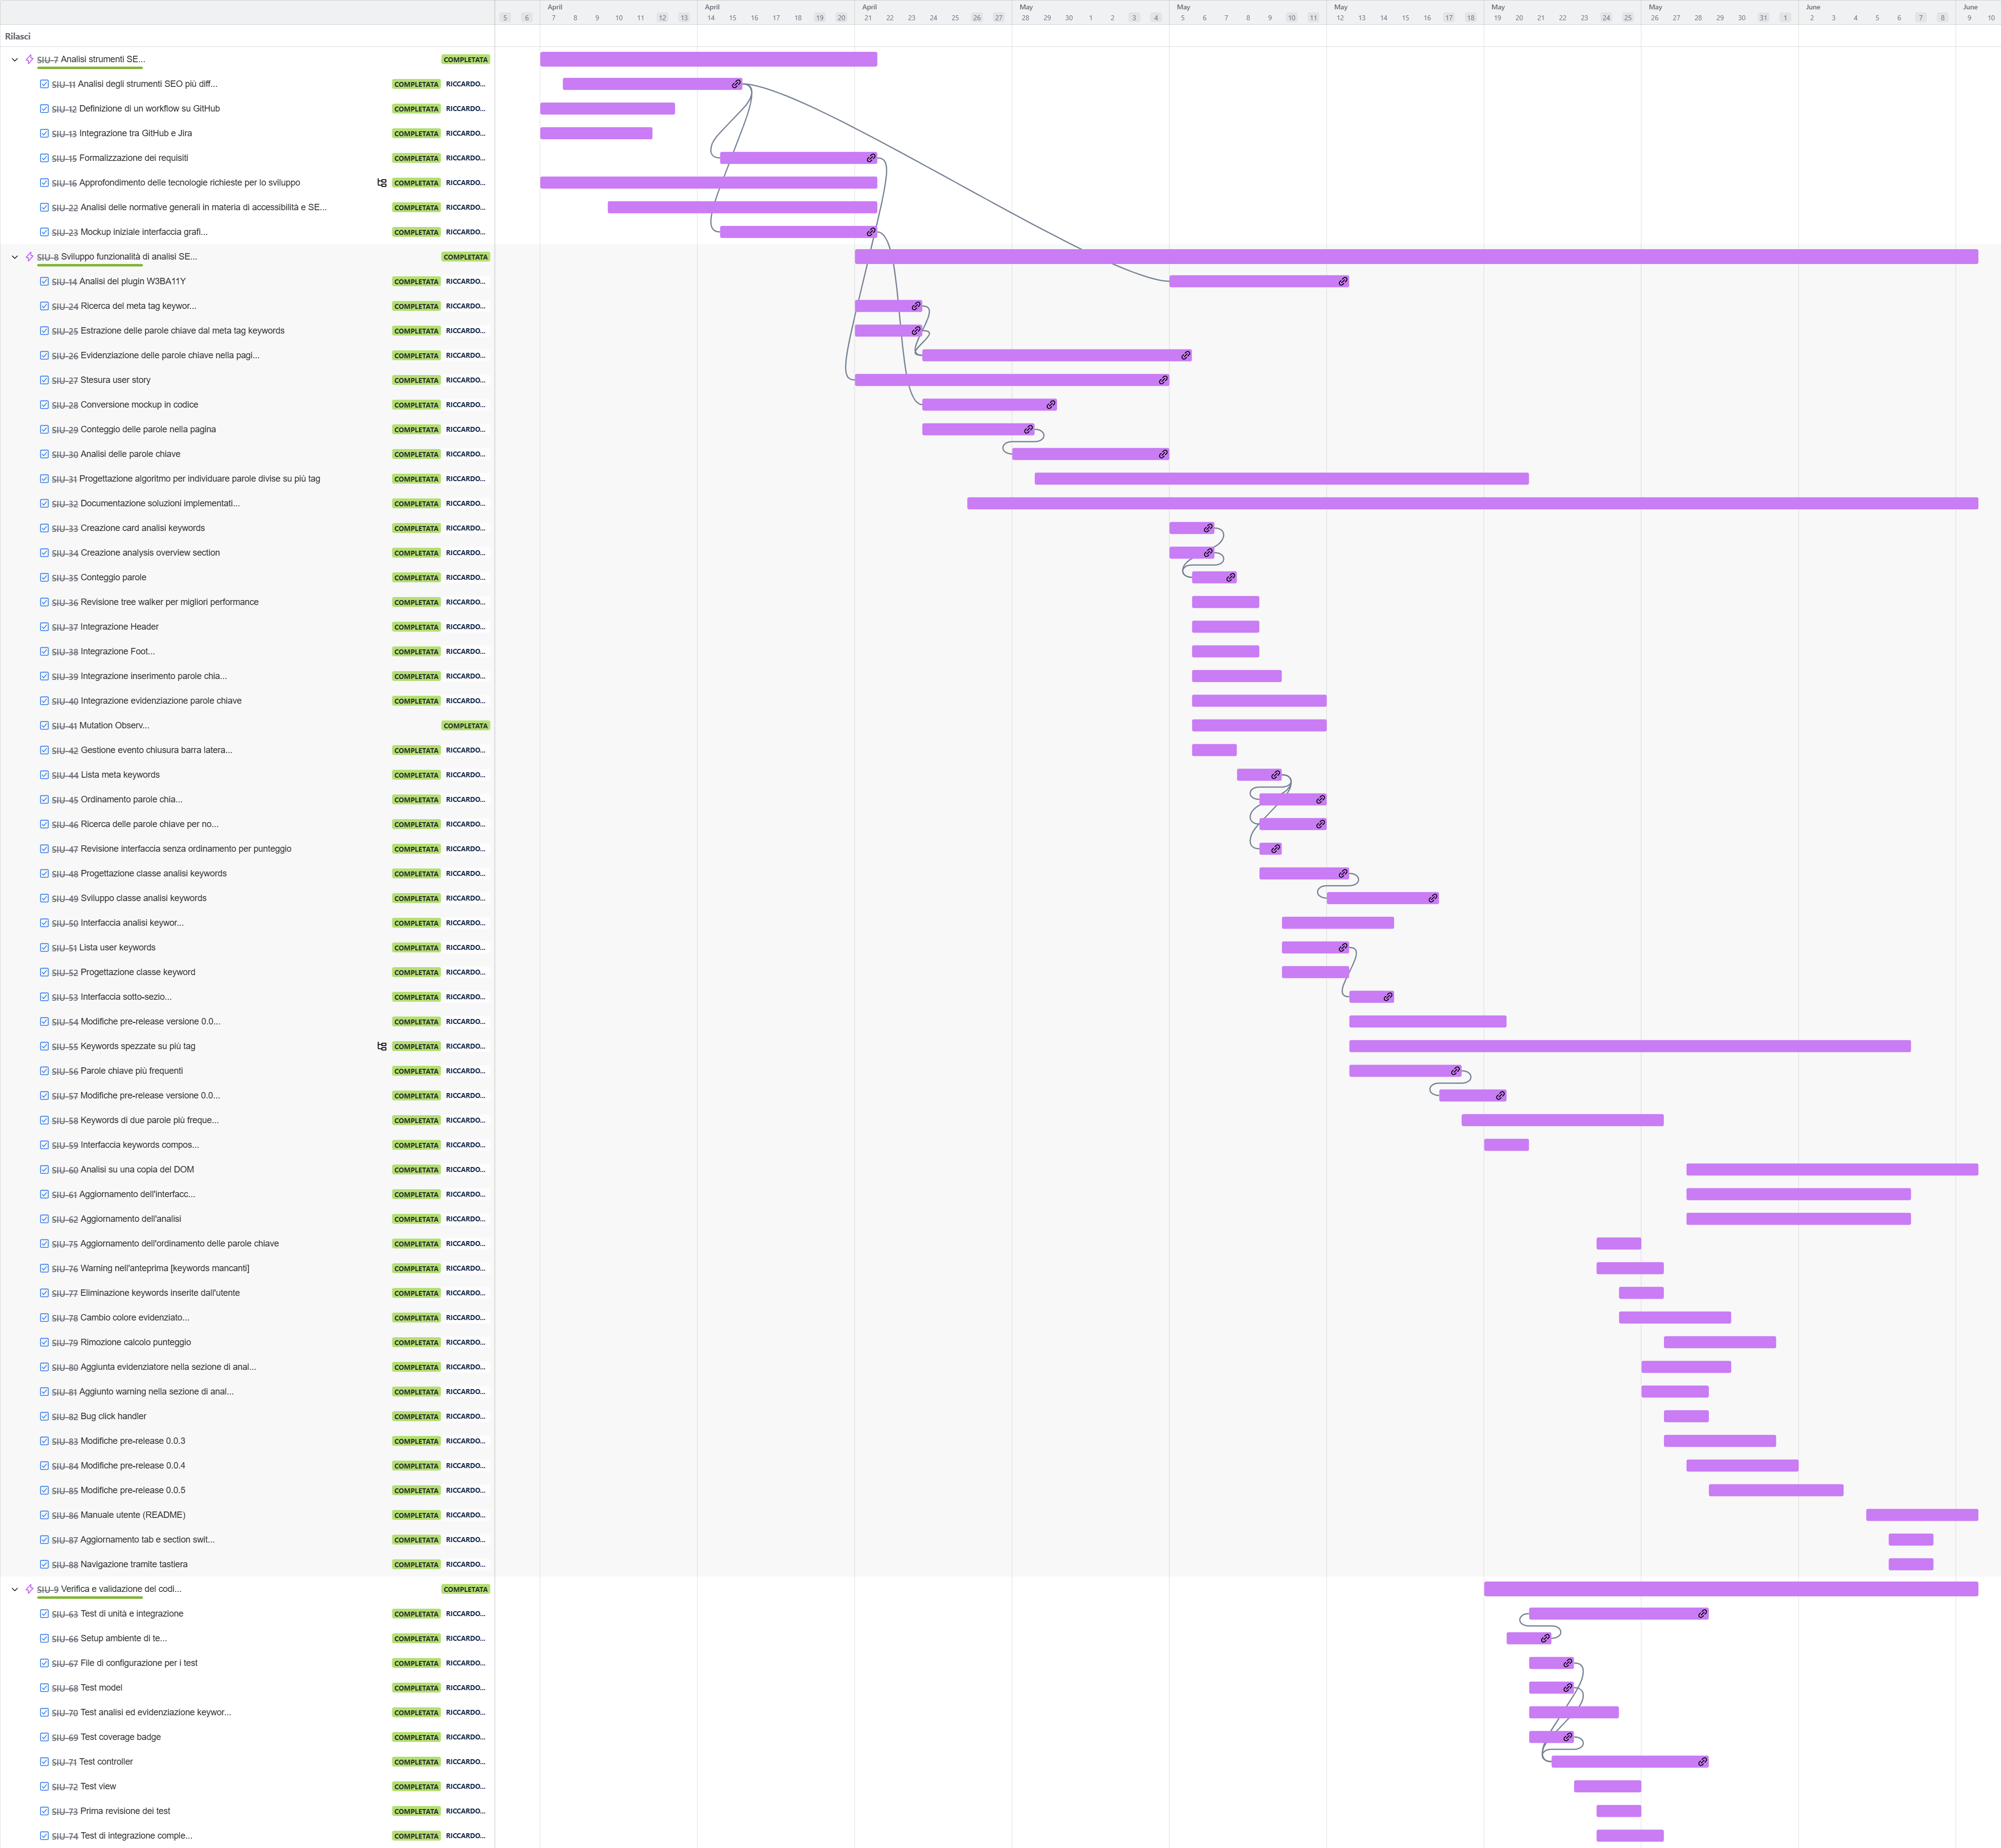
\includegraphics[width=0.8\columnwidth]{pianificazione/jira.png}} 
  \caption{Timeline Jira dal 07/04/2025 al 09/06/2025}
\end{figure}

\section{Strumenti e tecnologie}
\label{sec:strumenti-tecnologie}

\par Di seguito sono elencati, in ordine alfabetico, i principali strumenti e tecnologie utilizzati durante lo svolgimento del progetto.

\subsection{Strumenti}

\subsection*{Chrome DevTools}

\par Gli strumenti per sviluppatori di Chrome consentono di ispezionare, \textit{debuggare} e modificare le pagine web. Sono integrati direttamente nel browser e fungono da console di \textit{debug}, offrendo agli sviluppatori la possibilità di individuare rapidamente eventuali errori.

\begin{figure}[H]
    \centering 
    
\includegraphics[width=0.1\columnwidth]{strumenti-tecnologie/devtools_logo.png} 
\end{figure}

\subsection*{Codecov}

\par Codecov è un servizio di \textit{reporting} che monitora la copertura del codice, ovvero la percentuale di codice eseguito durante i test automatici. Nell’ambito del progetto di stage, è stato utilizzato per integrare queste informazioni direttamente nel flusso di lavoro su GitHub, in modo da garantire una copertura del codice uniforme per ogni \gls{pull request}. Inoltre, Codecov fornisce un \textit{badge} di stato utile ad arricchire la documentazione del \gls{repository}.

\begin{figure}[H]
    \centering 
    
\includegraphics[width=0.1\columnwidth]{strumenti-tecnologie/codecov_logo.pdf} 
\end{figure}

\subsection*{Draw.io}

\par Draw.io è uno strumento \textit{web-based} utilizzato per la creazione di sketch e diagrammi. La piattaforma è \textit{open source} e mette a disposizione template personalizzabili. I progetti possono essere salvati localmente oppure online, grazie all’integrazione con Google Workspace (Google Drive) e Dropbox. In assenza di una connessione a Internet, è disponibile un'applicazione desktop per macOS, Windows e Linux. Nell’ambito del progetto di stage, Draw.io è stato impiegato per la realizzazione dei diagrammi dei casi d’uso e delle classi.

\begin{figure}[H]
    \centering 
    
\includegraphics[width=0.2\columnwidth]{strumenti-tecnologie/draw_io_logo.pdf} 
\end{figure}

\subsection*{Figma}

\par Figma è uno strumento di progettazione e prototipazione, disponibile sia come servizio \textit{web-based} che come applicazione desktop. Due delle funzionalità più diffuse sono Figma Design, che consente di creare, condividere e testare i design in modo efficiente, e Dev Mode, che permette a designer e sviluppatori di collaborare strettamente per tradurre il design in codice. Nell’ambito dello stage, Figma è stato utilizzato per realizzare il \textit{mockup} dell’interfaccia grafica. Si è rivelato uno strumento di grande valore per la progettazione dell'interfaccia utente (UI) e dell’esperienza utente (UX), consentendo di analizzare lo spazio disponibile, organizzare gli elementi, scegliere i colori e costruire una base solida per lo sviluppo.

\begin{figure}[H]
    \centering 
    
\includegraphics[width=0.2\columnwidth]{strumenti-tecnologie/figma_logo.png} 
\end{figure}

\subsection*{GitHub}

\par Github è un servizio \textit{web e cloud-based} per l'archiviazione, il versionamento e la condivisione del codice. Nell’ambito dello stage, è stato utilizzato per contribuire allo sviluppo di un progetto preesistente tramite la funzionalità di \textit{fork}, che consente di lavorare sul codice in modo isolato, per poi proporre le modifiche al \gls{repository} originale. GitHub permette anche di aprire spazi di discussione relativi al codice tramite \textit{issue} e \gls{pull request}, oltre a fornire strumenti per la gestione del progetto come \textit{board} e \textit{milestone}. Inoltre, consente di automatizzare i flussi di lavoro attraverso le \textit{GitHub Actions}.

\begin{figure}[H]
    \centering 
    
\includegraphics[width=0.1\columnwidth]{strumenti-tecnologie/github_logo.pdf} 
\end{figure}

\subsection*{Google Docs}

\par Google Docs è un software \textit{web-based} per la scrittura e la condivisione di documenti. Nell’ambito del progetto di stage, è stato utilizzato per la redazione dei seguenti documenti: piano di lavoro, analisi degli strumenti \gls{seo}, analisi dei \gls{requisiti}, soluzioni progettuali e implementative.

\begin{figure}[H]
    \centering 
    
\includegraphics[width=0.1\columnwidth]{strumenti-tecnologie/google_docs_logo.pdf} 
\end{figure}

\subsection*{Google Drive}

\par Google Drive è uno strumento \textit{web-based}, parte di Google Workspace, che consente di archiviare, organizzare, condividere e accedere in modo sicuro a file e cartelle ovunque, da qualsiasi dispositivo connesso a Internet. Nell’ambito del progetto di stage, Google Drive è stato adottato come “unica fonte di verità”, ovvero come raccolta centralizzata di tutto il materiale condiviso tra stagista e Proponente (piano di lavoro, appunti, link utili, analisi dei \gls{requisiti}, soluzioni progettuali, diagrammi, ecc.).

\begin{figure}[H]
    \centering 
    
\includegraphics[width=0.1\columnwidth]{strumenti-tecnologie/google_drive_logo.pdf} 
\end{figure}

\subsection*{Google Forms}

\par Google Forms è uno strumento \textit{web-based} per la creazione di moduli, questionari, quiz e sondaggi. Nell’ambito del progetto di stage, è stato utilizzato per la creazione di un questionario \gls{sus} finalizzato alla valutazione dell’usabilità del software sviluppato.

\begin{figure}[H]
    \centering 
    
\includegraphics[width=0.1\columnwidth]{strumenti-tecnologie/google_forms_logo.pdf} 
\end{figure}

\subsection*{Google Sheets}

\par Google Sheets è un software \textit{web-based} per la creazione e la condivisione di fogli di calcolo. Nell’ambito del progetto di stage, è stato utilizzato per memorizzare le risposte al questionario \gls{sus} e per creare una tabella di calcolo dei punteggi.

\begin{figure}[H]
    \centering 
    
\includegraphics[width=0.1\columnwidth]{strumenti-tecnologie/google_sheets_logo.pdf} 
\end{figure}

\subsection*{Jira}

\par Jira è un'applicazione software sviluppata da Atlassian che consente agli utenti di gestire progetti, monitorare le attività e automatizzare i flussi di lavoro. È uno degli strumenti di gestione \textit{agile} più utilizzati, in particolare in contesti fortemente collaborativi, poiché risponde alle esigenze dei team di pianificare, monitorare, rilasciare e supportare software in modo sicuro. Nell’ambito dello stage, Jira è stato impiegato per la pianificazione e il monitoraggio delle tre fasi principali del progetto: analisi delle soluzioni esistenti, sviluppo e collaudo. L’integrazione con GitHub consente di tracciare i \textit{ticket} direttamente nell’ambiente di sviluppo e di automatizzarne la gestione. Inoltre, Jira mette a disposizione una \textit{timeline} che offre una panoramica immediata delle dipendenze tra le attività e del rispetto delle scadenze.

\begin{figure}[H]
    \centering 
    
\includegraphics[width=0.15\columnwidth]{strumenti-tecnologie/jira_logo.pdf} 
\end{figure}

\subsection*{npm}

\par npm (Node Package Manager) è un gestore di pacchetti per JavaScript che consente di gestire le dipendenze di un progetto. Tutti i pacchetti sono definiti nel file di configurazione \textit{package.json}. Nell’ambito dello stage, npm è stato utilizzato per configurare i test automatizzati tramite Jest e per gestire il versionamento del progetto.

\begin{figure}[H]
    \centering 
    
\includegraphics[width=0.15\columnwidth]{strumenti-tecnologie/npm_logo.pdf} 
\end{figure}

\subsection*{Visual Studio Code}

\par Visual Studio Code è un editor di codice sorgente, più leggero e flessibile rispetto a un ambiente di sviluppo integrato tradizionale. Combina la semplicità di un editor con \textit{feature} avanzate per sviluppatori, come il completamento del codice e altre funzionalità di assistenza alla scrittura.

\begin{figure}[H]
    \centering 
    
\includegraphics[width=0.1\columnwidth]{strumenti-tecnologie/vscode_logo.png} 
\end{figure}

\subsection{Tecnologie}

\subsection*{Chrome Extension APIs}

\par Le Chrome Extension APIs forniscono agli sviluppatori un insieme di interfacce che permettono di estendere e personalizzare le funzionalità del browser. Queste \gls{api} sono accessibili da qualsiasi componente dell’estensione. Consentono di accedere ai dati del browser, interagire con le schede, modificare il contenuto delle pagine web, memorizzare informazioni, gestire eventi e scambiare messaggi tra i componenti dell’estensione, ad esempio tra i \textit{background e i content script}.

\begin{figure}[H]
    \centering 
    
\includegraphics[width=0.15\columnwidth]{strumenti-tecnologie/chrome_extension_logo.png} 
\end{figure}

\subsection*{CSS}

\par CSS (Cascading Style Sheets) è un linguaggio utilizzato per definire lo stile e la formattazione di documenti scritti in linguaggi di markup come HTML o XML. Nell’ambito del progetto di stage, è stata adottata la versione CSS3.

\begin{figure}[H]
    \centering 
    
\includegraphics[width=0.25\columnwidth]{strumenti-tecnologie/css_logo.png} 
\end{figure}

\subsection*{HTML}

\par HTML (Hypertext Markup Language) è un linguaggio di markup utilizzato per definire la struttura e i contenuti delle pagine web. Nell’ambito del progetto di stage, è stata adottata la versione HTML5.

\begin{figure}[H]
    \centering 
    
\includegraphics[width=0.15\columnwidth]{strumenti-tecnologie/html_logo.png} 
\end{figure}

\subsection*{JavaScript}

\par JavaScript è un linguaggio di programmazione utilizzato per definire il comportamento e la logica delle pagine web. È un linguaggio multi-paradigma che può essere impiegato sia nella programmazione lato client che lato server (Node.js). JavaScript consente di aggiornare dinamicamente i contenuti HTML e gli stili CSS. Si integra perfettamente con \gls{framework} di test come Jest e strumenti di documentazione come JSDoc. È inoltre il linguaggio di riferimento per lo sviluppo di estensioni web.

\begin{figure}[H]
    \centering 
    \includegraphics[width=0.15\columnwidth]{strumenti-tecnologie/js_logo.png} 
\end{figure}

\subsection*{Jest}

\par Jest è un \gls{framework} di test per JavaScript, utilizzato per la progettazione, lo sviluppo e l’esecuzione di test di unità e di integrazione. Permette di definire suite di test efficienti e isolate, senza richiedere configurazioni complesse, anche quando viene integrato in progetti già avviati. Aggiungendo il flag \verb|--coverage|, è possibile generare un report sulla copertura del codice e inviare i risultati a strumenti di terze parti come Codecov. Nell’ambito del progetto di stage, Jest è stato utilizzato insieme alla libreria Jest DOM per ottenere una copertura completa del codice.

\begin{figure}[H]
    \centering 
    
\includegraphics[width=0.1\columnwidth]{strumenti-tecnologie/jest_logo.pdf} 
\end{figure}

\subsection*{Librerie di icone}

\par Per l’interfaccia grafica sono state utilizzate icone provenienti da tre librerie:
\begin{itemize}
  \item \textbf{Font Awesome}: una vasta libreria di icone vettoriali gratuite e a pagamento;
  \item \textbf{Heroicons}: una raccolta di icone \gls{svg} realizzate a mano dai creatori di \textit{Tailwind CSS};
  \item \textbf{Remix Icon}: una libreria \textit{open source} di icone vettoriali progettate per designer e sviluppatori.
\end{itemize}

\vspace{5pt}
\begin{center}
  \begin{minipage}{0.3\columnwidth}
    \centering
    
\includegraphics[width=0.6\columnwidth]{strumenti-tecnologie/heroicons_logo.pdf} 
  \end{minipage}
  \hfill
  \begin{minipage}{0.3\columnwidth}
    \centering
    
\includegraphics[width=0.2\columnwidth]{strumenti-tecnologie/font_awesome_logo.pdf} 
  \end{minipage}
  \hfill
  \begin{minipage}{0.3\columnwidth}
    \centering
    
\includegraphics[width=0.6\columnwidth]{strumenti-tecnologie/remixicon_logo.pdf} 
  \end{minipage}
\end{center}
\vspace{5pt}

\subsection*{Manifest (manifest.json)}

\par Il file \textit{manifest.json} svolge un ruolo cruciale nello sviluppo di estensioni web, poiché consente agli sviluppatori di definire le funzionalità dell’estensione e le autorizzazioni richieste. Si tratta di un file di configurazione in formato \gls{json} che specifica una serie di metadati, tra cui i permessi, le risorse necessarie, i \textit{background e i content script}.

\subsection*{Stopword (stopword.js)}

\par Stopword è un modulo JavaScript che consente di rimuovere le \gls{stopword} da un testo. Oltre alla funzione \textit{removeStopwords}, l’\gls{api} mette a disposizione identificatori univoci per accedere agli array di stopword associati a lingue specifiche, con supporto verificato per oltre 60 lingue. Il modulo è distribuito con licenza \textit{MIT}.
        \chapter{Processi e metodologie}
\label{cap:processi-metodologie}

\intro{In questa sezione viene illustrato l’approccio organizzativo adottato per il progetto, includendo le strategie implementate per automatizzare i processi.}

\section{Modello di sviluppo}

\par L’organizzazione del lavoro è stata gestita tramite la piattaforma Jira, utilizzando un template \textit{Kanban} semplificato. Questo modello fornisce una \textit{timeline}, una \textit{board} suddivisa nelle etichette “Da completare”, “In corso” e “Completato” (analogamente a Trello), un calendario e una \textit{dashboard} per monitorare l’integrazione con \gls{github}. Il progetto è stato suddiviso in tre \textit{epic}, o macro-fasi (analisi, sviluppo, validazione), ciascuna delle quali si è conclusa con il rilascio di un prodotto. Ogni rilascio di documentazione o software è stato associato a una specifica \textit{milestone}. Il tempo dedicato ai tre \textit{epic} è stato ulteriormente articolato in periodi settimanali (simili agli \textit{sprint} della metodologia \textit{agile}). Questo approccio ha permesso di mantenere un rapporto costante con la Proponente; al termine di ogni periodo è stato fornito un aggiornamento sullo stato di avanzamento, in presenza o da remoto (tramite comunicazione via e-mail), e sono state pianificate le attività successive. La priorità delle attività è stata concordata settimanalmente con la Proponente, così da definire un elenco ordinato (simile a un \textit{backlog}) di \textit{task} da completare entro la fine dell’iterazione.

\section{Workflow GitHub}

\par Per gestire lo sviluppo, ho adottato una struttura basata su due \textit{branch} principali: \textit{main} e \textit{develop}. Il \textit{branch main} registra la cronologia dei rilasci e contiene codice stabile, pronto per la produzione, mentre \textit{develop} rappresenta la linea di sviluppo principale. A ciascuna funzionalità da implementare è associato un \textit{branch} dedicato, contraddistinto dal prefisso \textit{feature/}, che ne accompagna lo sviluppo fino all’integrazione in un ramo condiviso. Quando una funzionalità risulta completa o pronta per l’integrazione, viene sottoposta a revisione tramite l’apertura di una \gls{pull request}, che può essere arricchita con commenti, etichette, \textit{issue} e \textit{milestone}.

\vspace{10pt}
\par\noindent Questo flusso di lavoro è riconducibile al modello \textit{Gitflow}, introdotto da Vincent Driessen nel 2010. Nell’ambito del progetto di stage, il modello \textit{Gitflow} non è stato applicato in modo rigido, ma ibridato con alcuni principi dello sviluppo \textit{trunk-based}. Idealmente, \textit{Gitflow} prevede \textit{branch} isolati e di lunga durata, mentre l’approccio \textit{trunk-based} favorisce aggiornamenti piccoli e frequenti, anche in assenza del completamento di una funzionalità, sfruttando appieno il potenziale della \gls{continuous integration}.

\vspace{10pt}
\par\noindent Per avviare il rilascio di una nuova versione, \textit{Gitflow} prevede la creazione di un \textit{branch} con il prefisso \textit{release/}. Il rilascio vero e proprio si concretizza con l’integrazione nel \textit{branch main}, che viene contrassegnato con un numero di versione. La versione può essere etichettata come “latest” oppure “pre-release”, qualora non sia ancora pronta per l’ambiente di produzione. Al termine del rilascio, i due \textit{branch} principali, \textit{main} e \textit{develop}, devono essere riallineati.

\section{Workflow Jira}

\par Prima di creare un branch su \gls{github}, a ciascuna funzionalità viene associato un \textit{ticket}, che può essere arricchito con commenti, etichette, date di inizio e fine, ed eventuali sotto-ticket. La creazione del \textit{branch} può avvenire direttamente da Jira, così da garantire un collegamento automatico con il relativo \textit{ticket}. In alternativa, il collegamento tra un \textit{ticket} e un \textit{branch}, un \gls{commit} o una \gls{pull request} può essere stabilito inserendo l’ID del \textit{ticket} come commento. Se l’ID viene racchiuso tra parentesi quadre (es. [ID]) all’interno della sezione commenti di una \gls{pull request}, il \textit{bot} di Jira genera automaticamente un collegamento ipertestuale al progetto.

\section{Automatizzazione dei processi}

\par Ho configurato un \textit{workflow}, tramite \textit{GitHub Actions}, che si attiva a ogni apertura, aggiornamento o chiusura di una \gls{pull request}. Il \textit{workflow}, scritto in \gls{yaml}, avvia due \textit{job} principali: l’esecuzione dei test automatizzati e il monitoraggio della \textit{code coverage}. Per i test è stato adottato il \gls{framework} Jest, che produce automaticamente un report sulla copertura del codice. Il report viene inviato a Codecov, che aggiorna la \textit{dashboard} del progetto, genera un \textit{badge} di stato e pubblica un riepilogo nei commenti della \gls{pull request}. Il superamento dei test e il mantenimento della copertura (rispetto alla versione precedente) rappresentano condizioni necessarie per procedere con il \textit{merge}. Questo approccio promuove la \gls{continuous integration} e fornisce una valutazione oggettiva della qualità del codice.

\vspace{10pt}
\par\noindent Su Jira ho definito tre regole di automazione:
\begin{itemize}
  \item \textbf{PR\_merged}: si attiva quando viene eseguito il \textit{merge} di una \gls{pull request} e sposta i \textit{ticket} collegati dallo stato corrente a “Completato”;
  \item \textbf{TICKET\_closed}: si attiva quando tutti i \textit{ticket} subordinati risultano completati e sposta l'elemento principale dallo stato corrente a “Completato”;
  \item \textbf{TICKET\_reopened}: si attiva quando un \textit{ticket} subordinato viene (ri)aperto e sposta l’elemento principale dallo stato “Completato” a “In corso”.
\end{itemize}

\begin{figure}[H] 
  \centering 
  \fbox{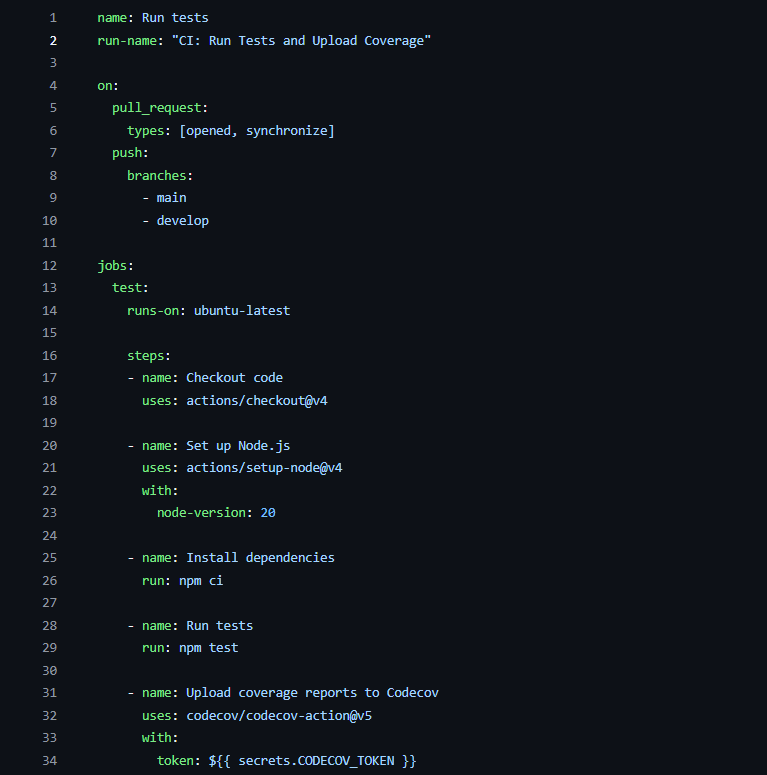
\includegraphics[width=0.9\textwidth]{processi/workflow.png}}
  \caption{Workflow YAML per continuous integration}
\end{figure}
        \chapter{Analisi del contesto tecnologico}
\label{cap:analisi-soluzioni-esistenti}

\par Uno dei passi fondamentali nel processo di ottimizzazione \gls{seo} è la scelta delle parole chiave e il loro utilizzo in punti strategici delle pagine web. Esistono software in grado di automatizzare la ricerca e l'analisi delle parole chiave, contribuendo a migliorare il posizionamento e l'indicizzazione di un sito. Questi strumenti, disponibili gratuitamente o a pagamento, coprono numerosi aspetti dell'analisi \gls{seo}, tra cui:
\begin{itemize}
    \item Analisi \gls{seo} \gls{on-page} e \gls{off-page};
    \item Identificazione delle parole chiave più frequenti;
    \item Analisi della densità e della distribuzione delle parole chiave all'interno di una pagina web;
    \item Analisi dell'efficacia delle parole chiave;
    \item Ricerca delle parole chiave per cui un sito è posizionato in alto nella \gls{serp};
    \item Suggerimenti di parole chiave correlate e rilevanti;
    \item Anteprime \gls{serp} per una determinata parola chiave;
    \item Analisi dei \textit{competitor};
    \item Analisi di parametri come la \gls{keyword-difficulty} e di pratiche come il \gls{keyword-stuffing}.
\end{itemize}

\section{MozBar}

\subsection{Funzionalità}
\par \textit{MozBar} è un'estensione gratuita per Chrome che consente agli utenti di eseguire analisi \gls{seo} \gls{on-page} e \gls{off-page} senza aprire un'altra scheda del browser. Le funzionalità fornite dall'estensione includono:
\begin{itemize}
    \item \textbf{Page Authority e Domain Authority}: metriche da 1 a 100 che stimano il posizionamento di una singola pagina o di un dominio in base a un algoritmo di apprendimento automatico;
    \item \textbf{Linking Domains}: numero di domini unici che puntano a un sito;
    \item \textbf{Inbound Links}: numero di link in entrata provenienti da pagine web esterne;
    \item \textbf{Attributi generali}: tempo di caricamento, \gls{tag-canonical}, URL della cache di Google, \gls{sitemap}, \gls{hreflang}, \gls{tag-robots};
    \item \textbf{Elementi on-page}: URL, titolo, meta description, meta tag keywords, elenco degli heading, testo alternativo delle immagini;
    \item \textbf{Dati strutturati (\gls{json-ldg})}: verifica che lo schema sia formattato correttamente;
    \item \textbf{Ranking Keywords}: identifica le parole chiave per cui un sito è posizionato e fornisce informazioni sui \textit{competitor};
    \item \textbf{Ottimizzazione della pagina}: visualizza il punteggio ottenuto per una determinata parola chiave e mostra  i fattori che contribuiscono al punteggio complessivo, nonché quelli che potrebbero danneggiarlo;
    \item \textbf{Highlight links}: evidenzia tutte le tipologie di link presenti all'interno della pagina;
    \item \textbf{Highlight keywords}: questa funzionalità, rappresentata in figura \ref{fig:mozbar}, consente agli utenti di inserire una parola chiave e ottenere il numero di occorrenze. Inoltre, permette di evidenziare graficamente una parola chiave all'interno della pagina.
\end{itemize}

\begin{figure}[H]
    \centering 
    \fbox{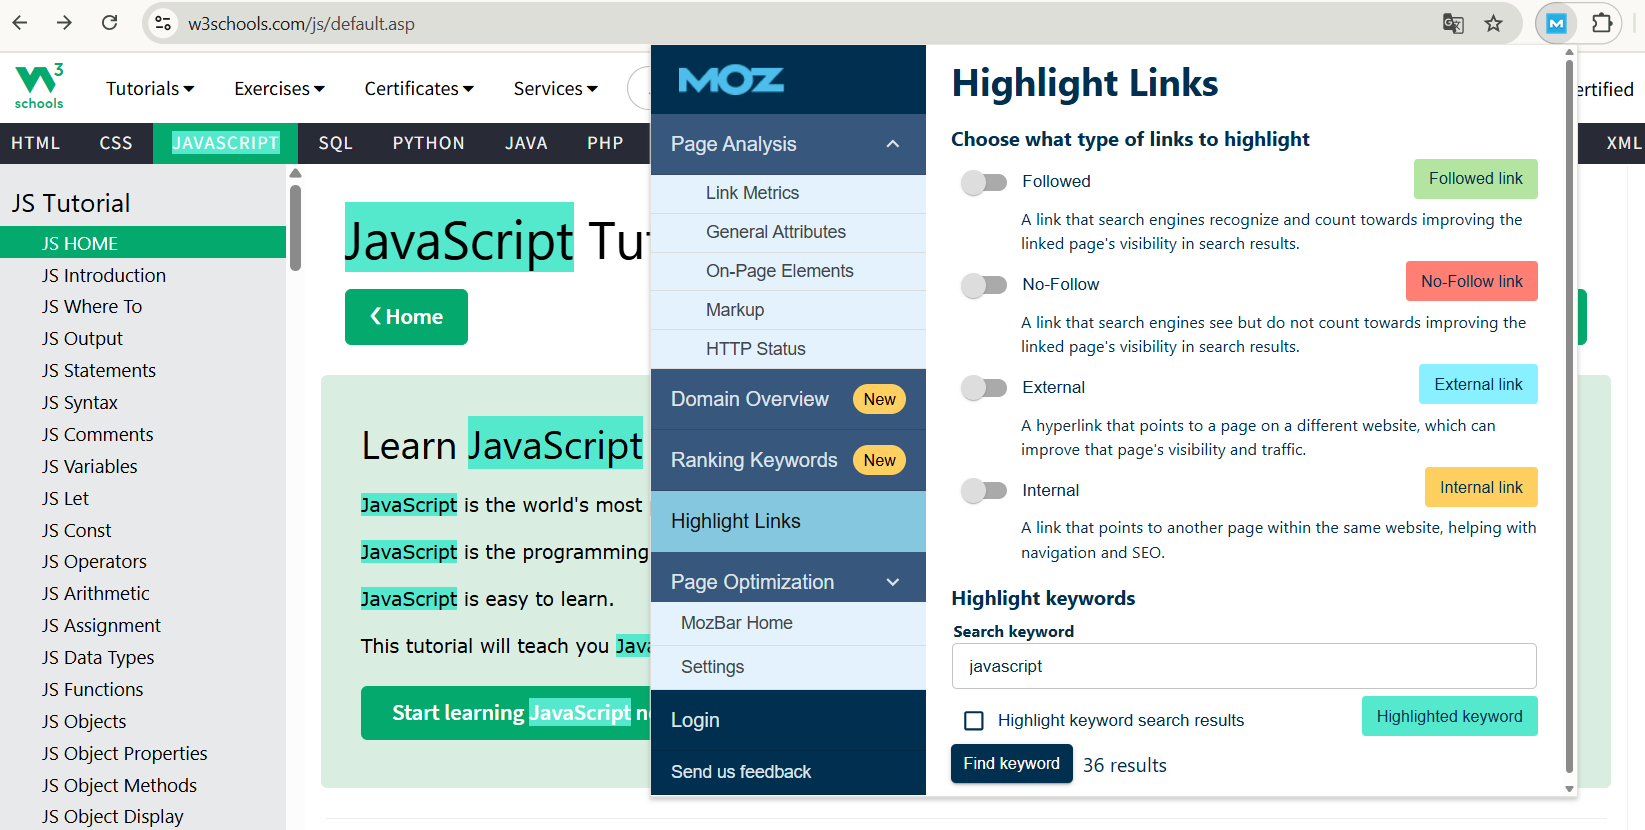
\includegraphics[width=0.9\columnwidth]{soluzioni-esistenti/MozBar/moz_bar_search_keywords.png}}
    \caption{MozBar - Analisi del sito “W3Schools”}
    \label{fig:mozbar}
\end{figure}

\subsection{Vantaggi}
\par Poiché funziona su \gls{localhost}, l'estensione può essere facilmente usata durante lo sviluppo. La barra degli strumenti può essere ancorata in alto o in basso nella pagina e le metriche \gls{seo} possono essere visualizzate direttamente nei risultati di ricerca.

\subsection{Svantaggi}
\par L'estensione non è disponibile come barra laterale, ma solo come pop-up o barra degli strumenti. L'analisi delle parole chiave non include alcuni aspetti essenziali, come la densità o la distribuzione. Inoltre, il rilevamento dei tag è \gls{case-sensitive}, quindi c'è il rischio che alcuni tag non vengano individuati se si usa la lettera iniziale maiuscola. Le funzionalità Premium richiedono un abbonamento a pagamento. 

\section{Wincher}

\subsection{Funzionalità}
\par \textit{Wincher} è una piattaforma orientata alla ricerca e all'analisi delle parole chiave; in particolare, \textit{Wincher} monitora il posizionamento di un sito web, i volumi di ricerca, il traffico stimato e le anteprime \gls{serp}. La piattaforma include anche l'\textit{On-Page SEO Checker}, uno strumento di analisi \gls{on-page} per un URL e una parola chiave specifici. Il \textit{tool}, rappresentato in figura \ref{fig:on_page_seo_checker}, fornisce suggerimenti per migliorare una pagina web in relazione alla parola chiave scelta:
\begin{itemize}
    \item \textbf{Titolo}: lunghezza del titolo, presenza e posizione della parola chiave nel titolo;
    \item \textbf{Heading}: lunghezza e numero di occorrenze del tag H1, presenza e posizione della parola chiave nel tag H1, differenza di contenuto tra il titolo e il tag H1, presenza della parola chiave nei sottotitoli;
    \item \textbf{Meta}: presenza della parola chiave nel meta tag description;
    \item \textbf{Media}: presenza della parola chiave nel testo alternativo delle immagini;
    \item \textbf{URL}: presenza della parola chiave negli URL;
    \item \textbf{Body}: la parola chiave dovrebbe essere menzionata almeno tre volte nel corpo del testo.
\end{itemize}

\begin{figure}[H]
    \centering 
    \fbox{
\includegraphics[width=0.8\columnwidth]{soluzioni-esistenti/Wincher/wincher_seo_checker.png}}
    \caption{Wincher - On-Page SEO Checker}
    \label{fig:on_page_seo_checker}
\end{figure}

\subsection{Vantaggi}
\par \textit{On-Page SEO Checker} fornisce un punteggio complessivo e dei suggerimenti per garantire la conformità di una pagina alle attuali linee guida \gls{seo}.

\subsection{Svantaggi}
\par Lo strumento di analisi \gls{on-page} non funziona su \gls{localhost} ed è accessibile esclusivamente tramite la piattaforma di \textit{Wincher}. Nella versione gratuita, i controlli giornalieri sono limitati.

\vspace{10pt}
\par\noindent La figura \ref{fig:wincher_w3schools} mostra un esempio di analisi del sito “W3Schools” effettuata con \textit{Wincher}.

\begin{figure}[H]
    \centering 
    \fbox{
\includegraphics[width=0.8\columnwidth]{soluzioni-esistenti/Wincher/wincher_seo_checker_score.png}}
    \caption{Wincher - Analisi del sito “W3Schools”}
    \label{fig:wincher_w3schools}
\end{figure}

\section{SEOquake}

\subsection{Funzionalità}
\par \textit{SEOquake} è un plugin che fornisce metriche \gls{seo} e strumenti di analisi \gls{on-page}. Le parole chiave vengono identificate tramite un algoritmo di ricerca e successivamente elencate in quattro tabelle distinte:
\begin{itemize}
    \item Keyword di 1 parola;
    \item Keyword di 2 parole;
    \item Keyword di 3 parole;
    \item Keyword di 4 parole.
\end{itemize}
\vspace{5pt}
\par\noindent Per ogni parola chiave, \textit{SEOquake} visualizza il numero di occorrenze e la densità. Inoltre, verifica se ciascuna parola chiave appare nei seguenti tag \gls{html}:
\begin{itemize}
    \item Titolo della pagina;
    \item Meta description;
    \item Meta tag keywords;
    \item Tag H1.
\end{itemize}
\vspace{5pt}
\par\noindent Tutti questi fattori contribuiscono a determinare un punteggio di importanza per ogni parola chiave. \textit{SEOquake} permette anche di filtrare le parole chiave, esportare i risultati dell'analisi in formato \gls{csv} e configurare un elenco di parole da includere o escludere. La figura \ref{fig:seoquake_w3schools} mostra un esempio di analisi del sito “W3Schools” effettuata con \textit{SEOquake}.

\begin{figure}[H]
    \centering 
    \fbox{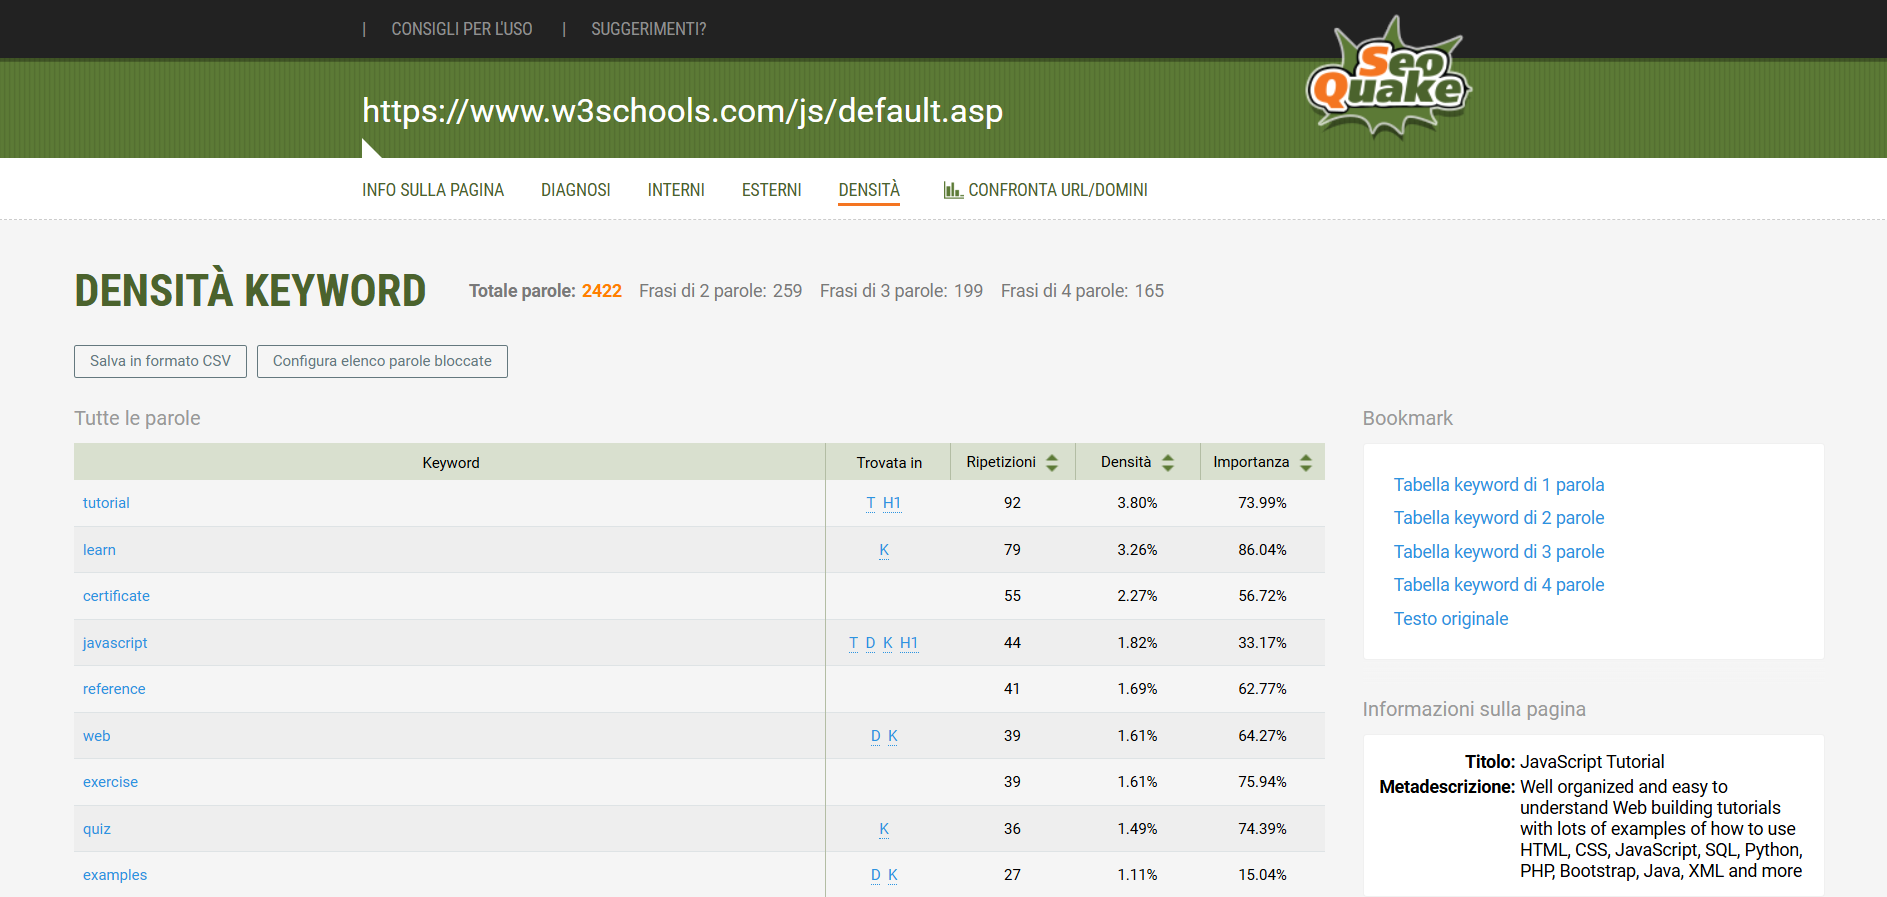
\includegraphics[width=0.9\columnwidth]{soluzioni-esistenti/SEOquake/seoquake.png}} 
    \caption{SEOquake - Analisi del sito “W3Schools”}
    \label{fig:seoquake_w3schools}
\end{figure}

\subsection{Vantaggi}
\par Oltre all'analisi \gls{on-page}, \textit{SEOquake} offre anche funzionalità avanzate come l'analisi dei \gls{backlink} e del traffico; il tutto è integrato in un'unica piattaforma che funziona su \gls{localhost}. L'estensione è sviluppata da \textit{Semrush} e, pertanto, include servizi propri della piattaforma.

\subsection{Svantaggi}
\par Le funzionalità di analisi \gls{seo} \gls{on-page} sono accessibili solo tramite la \textit{dashboard} esterna, il che limita l'interazione diretta con la pagina corrente.

\section{SEOptimer}

\subsection{Funzionalità}
\par \textit{SEOptimer} è una piattaforma di analisi \gls{seo} e reportistica. Offre una suite completa di strumenti che coprono le seguenti funzionalità:
\begin{itemize}
    \item \textbf{Audit SEO}: fornisce un punteggio complessivo basato su fattori come \gls{seo} \gls{on-page} e \gls{off-page}, usabilità, performance e ottimizzazione per i social media;
    \item \textbf{Crawler SEO}: esegue una scansione dettagliata di una pagina web, includendo un'analisi della distribuzione delle parole chiave. Le parole chiave vengono estratte in base alla frequenza e suddivise in:
    \begin{itemize}
        \item Keyword di 1 parola;
        \item Keyword di 2 o più parole.
    \end{itemize}
    Le parole chiave dovrebbero essere distribuite correttamente tra i seguenti tag \gls{html}: 
    \begin{itemize}
        \item Titolo della pagina;
        \item Meta description;
        \item Tag di intestazione (heading).
    \end{itemize}
    \item \textbf{Monitoraggio delle parole chiave};
    \item \textbf{Ricerca di parole chiave}: analizza i \textit{competitor} e fornisce suggerimenti per nuove parole chiave;
    \item \textbf{Ricerca e monitoraggio dei \gls{backlink}}.
\end{itemize}

\vspace{10pt}
\par\noindent La figura \ref{fig:seoptimer_w3schools} mostra un esempio di analisi del sito “W3Schools” effettuata con \textit{SEOptimer}.

\begin{figure}[H]
    \centering 
    \fbox{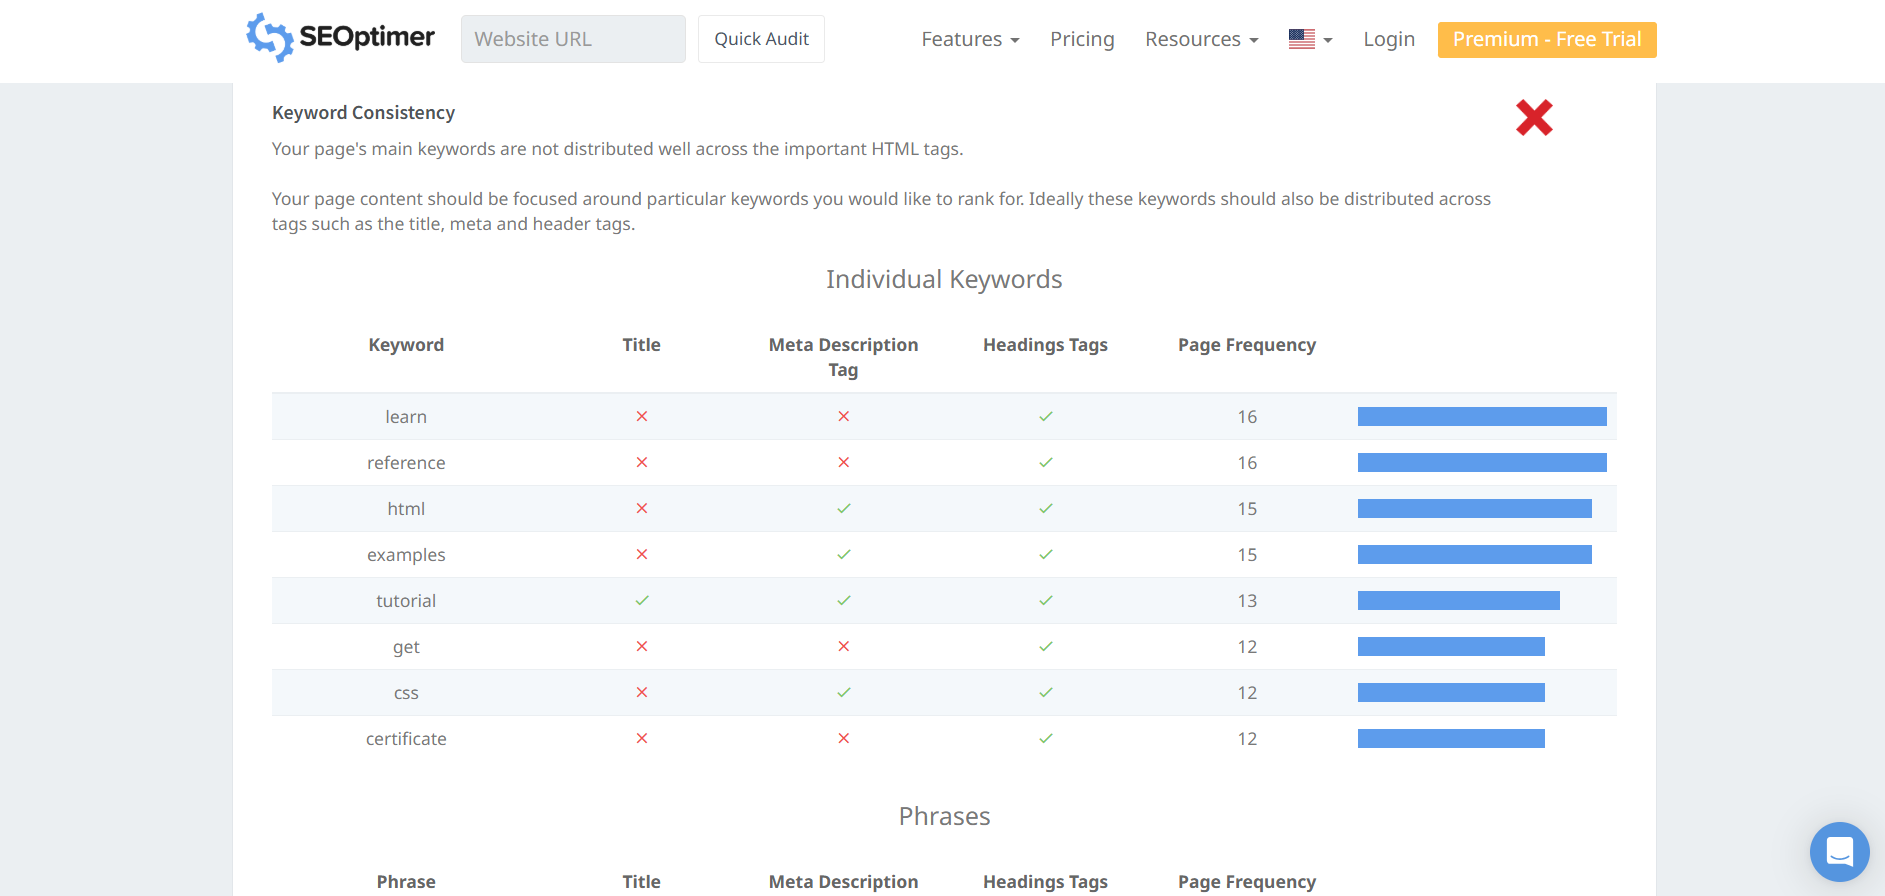
\includegraphics[width=0.9\columnwidth]{soluzioni-esistenti/SEOptimer/seoptimer.png}} 
    \caption{SEOptimer - Analisi del sito “W3Schools”}
    \label{fig:seoptimer_w3schools}
\end{figure}

\subsection{Vantaggi}
\par \textit{SEOptimer} integra in un'unica piattaforma tutti gli strumenti necessari per un'analisi \gls{seo} approfondita ed è più economico rispetto ad altri servizi simili.

\subsection{Svantaggi}
\par \textit{SEOptimer} non funziona su \gls{localhost} e la versione gratuita consente un numero limitato di report giornalieri. Non è disponibile un'estensione per browser, pertanto l'analisi può essere eseguita soltanto tramite la piattaforma proprietaria.

\section{SEO tester online}

\subsection{Funzionalità}
\par \textit{SEO tester online} è un'estensione gratuita per Chrome sviluppata da \textit{Sitechecker}. Fornisce una panoramica generale dei dati \gls{seo} essenziali, seguita da un elenco di sezioni specifiche, tra cui:
\begin{itemize}
    \item \textbf{Contenuto}: analizza la gerarchia degli heading, la lunghezza del testo, il rapporto testo/codice \gls{html} e la densità delle keyword composte da 1, 2 o 3 parole;
    \item \textbf{Link e immagini};
    \item \textbf{\Gls{hreflang} e dati strutturati};
    \item \textbf{Velocità di caricamento};
    \item \textbf{Analisi \gls{gsc}}.
\end{itemize}

\subsection{Vantaggi}
\par L'estensione è gratuita e si integra con \gls{gsc}, offrendo un'analisi \gls{seo} completa e professionale.

\subsection{Svantaggi}
\par L'estensione non funziona su \gls{localhost} e si apre unicamente come pop-up.

\vspace{10pt}
\par\noindent La figura \ref{fig:seo_tester_online_w3schools} mostra un esempio di analisi del sito “W3Schools” effettuata con \textit{SEO tester online}.

\begin{figure}[H]
    \centering 
    \fbox{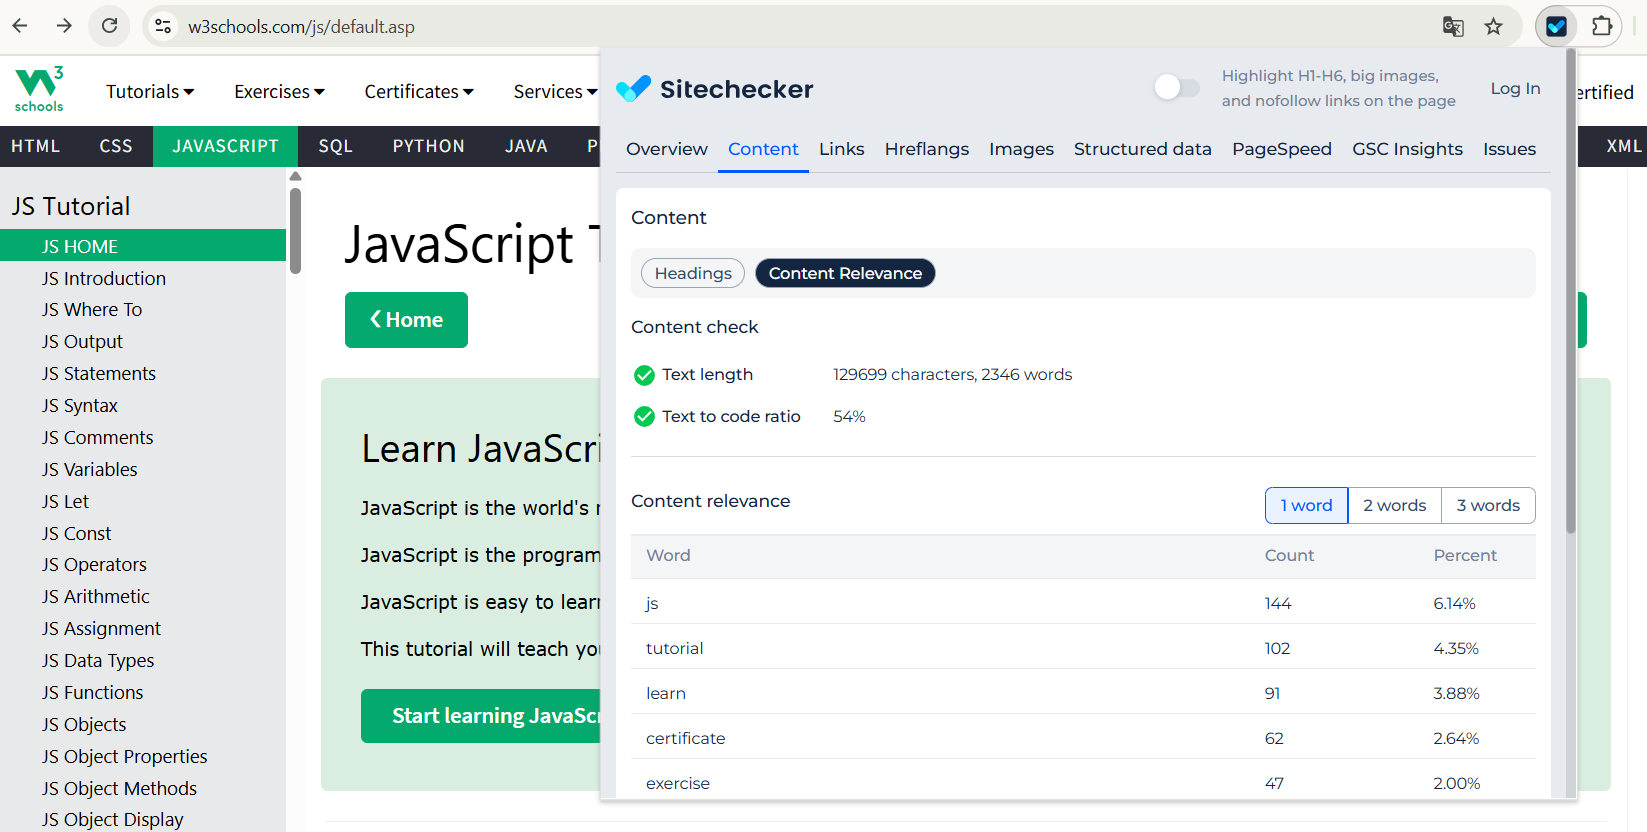
\includegraphics[width=0.9\columnwidth]{soluzioni-esistenti/SEO-Tester-Online/site_checker.png}} 
    \caption{SEO tester online - Analisi del sito “W3Schools”}
    \label{fig:seo_tester_online_w3schools}
\end{figure}

\section{Semrush}

\subsection{Funzionalità}
\par \textit{Semrush} include oltre 50 strumenti di analisi \gls{seo}, il che lo rende una delle piattaforme più complete sul mercato. La \textit{dashboard}, mostrata in figura \ref{fig:semrush}, consente di visualizzare gratuitamente analisi relative al traffico, ai \gls{backlink}, alle ricerche \gls{organiche} e a quelle \gls{sponsorizzate}. In merito all’analisi delle parole chiave, \textit{Semrush} offre le seguenti funzionalità:
\begin{itemize}
    \item \textbf{Analisi SEO on-page};
    \item \textbf{Keyword research}: suggerisce parole chiave rilevanti in base al volume di ricerca, all'intento, alla \gls{keyword-difficulty} e ad altri fattori \gls{seo}. Questa funzionalità può essere integrata con plugin di terze parti, tra cui \textit{Yoast SEO} per \gls{wordpress};
    \item \textbf{Analisi dei competitor};
    \item \textbf{Position tracking}: monitora il posizionamento nella \gls{serp} per determinate parole chiave.
\end{itemize}

\begin{figure}[H] 
    \centering 
    \fbox{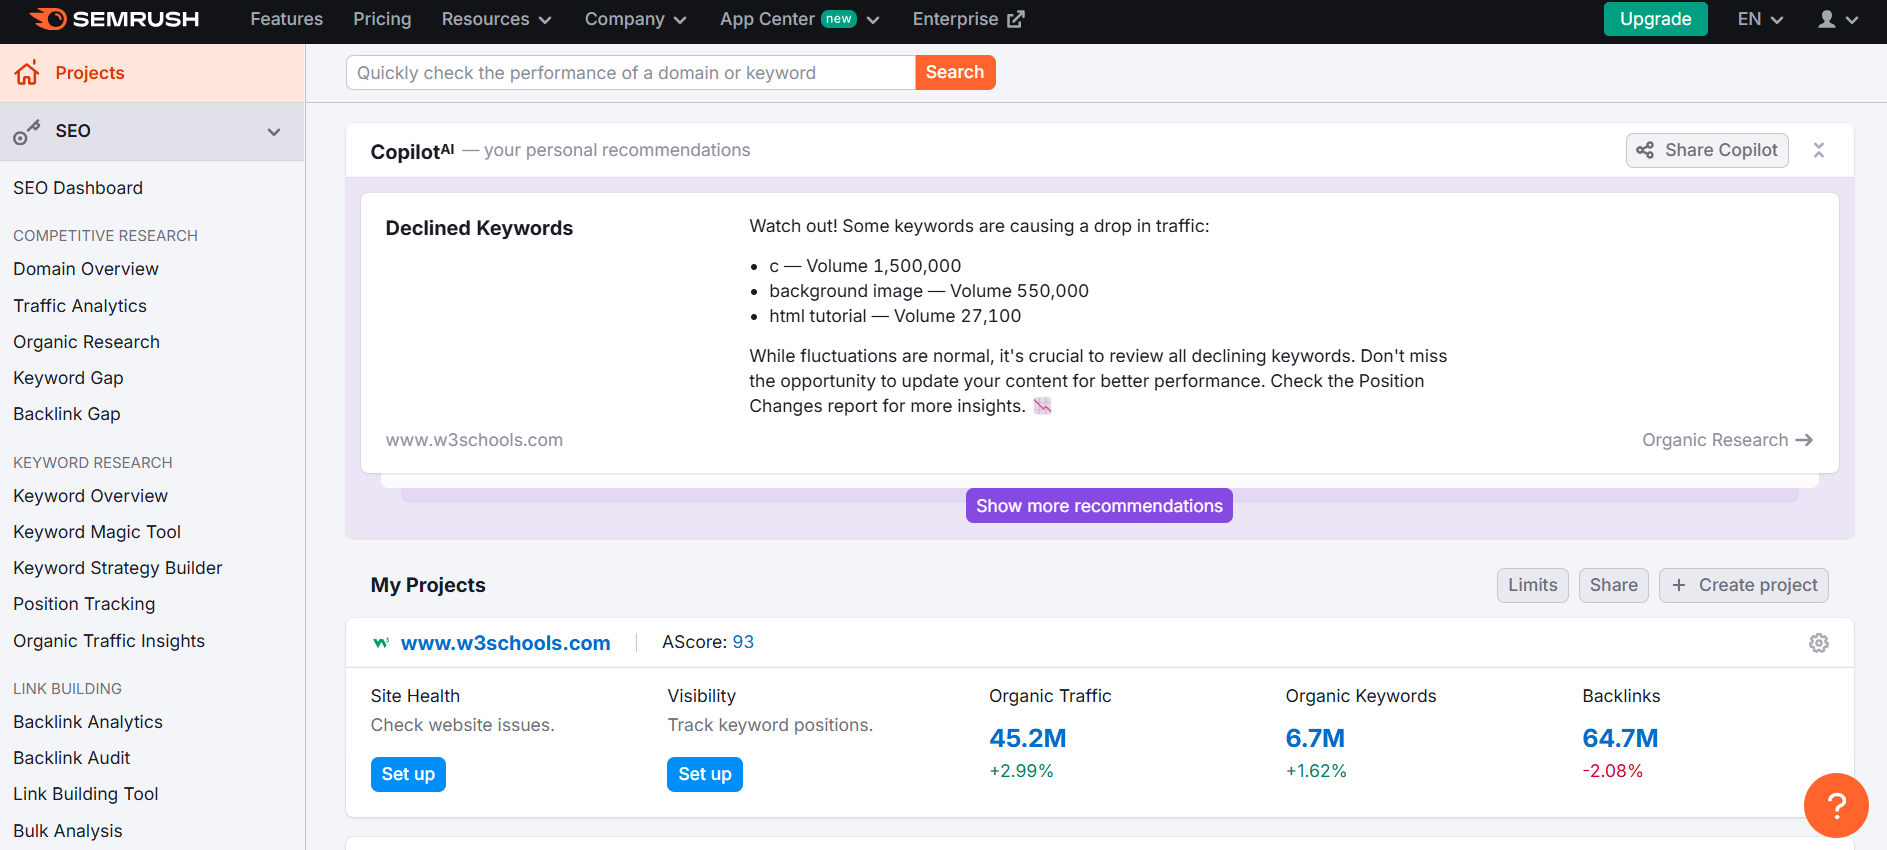
\includegraphics[width=0.8\textwidth]{soluzioni-esistenti/SEMrush/semrush.png}} 
    \caption{Semrush - SEO dashboard}
    \label{fig:semrush}
\end{figure}

\subsection{Vantaggi}
\par \textit{Semrush} può essere integrato facilmente con altri strumenti di analisi \gls{seo}.

\subsection{Svantaggi}
\par Le funzionalità avanzate sono a pagamento. Per effettuare un'analisi, è necessario interrompere la navigazione e accedere alla piattaforma web di \textit{Semrush}.

\section{Yoast SEO (plugin per CMS)}

\subsection{Funzionalità}
\par \textit{Yoast SEO} è un plugin per \gls{cms} che semplifica il processo di ottimizzazione \gls{seo}. Fornisce feedback in tempo reale per migliorare il posizionamento sui motori di ricerca. La versione del plugin per \gls{wordpress} consente di ottimizzare le parole chiave (note anche come keyphrase) attraverso un'analisi della densità, della distribuzione e di altri fattori \gls{on-page}. Con la versione a pagamento, l'utente può anche scegliere manualmente delle keyphrase correlate (argomenti collegati o parole chiave secondarie) da valutare distintamente. Inoltre, l'integrazione con \textit{Semrush} fornisce automaticamente suggerimenti di keyphrase correlate basati sui volumi di ricerca, sull'intento e sulla \gls{keyword-difficulty}. Naturalmente, i controlli sono meno restrittivi rispetto alla keyphrase principale. Per evitare di dover ripetere meccanicamente la stessa keyphrase, la versione Premium permette anche di aggiungere uno o più sinonimi, che \textit{Yoast} interpreta allo stesso modo senza penalizzare il punteggio.

\subsection{Vantaggi}
\par \textit{Yoast SEO} è disponibile in versione gratuita per \gls{wordpress}, seppur con alcune limitazioni, e può essere integrato con altri strumenti come \textit{Semrush} e \textit{Wincher}. Il plugin viene aggiornato regolarmente per rimanere allineato agli algoritmi dei motori di ricerca e alle \textit{best practice} \gls{seo}.

\subsection{Svantaggi}
\par \textit{Yoast SEO} è limitato a \gls{cms} come \gls{wordpress} e \gls{shopify}. Alcune funzionalità, tra cui l'inserimento di keyphrase correlate e sinonimi, o l'integrazione con \textit{Semrush}, richiedono la sottoscrizione di un abbonamento a pagamento.

\vspace{10pt}
\par\noindent La figura \ref{fig:yoast_seo} mostra un esempio di analisi effettuata con \textit{Yoast SEO Premium}.

\begin{figure}[H]
    \centering 
    \fbox{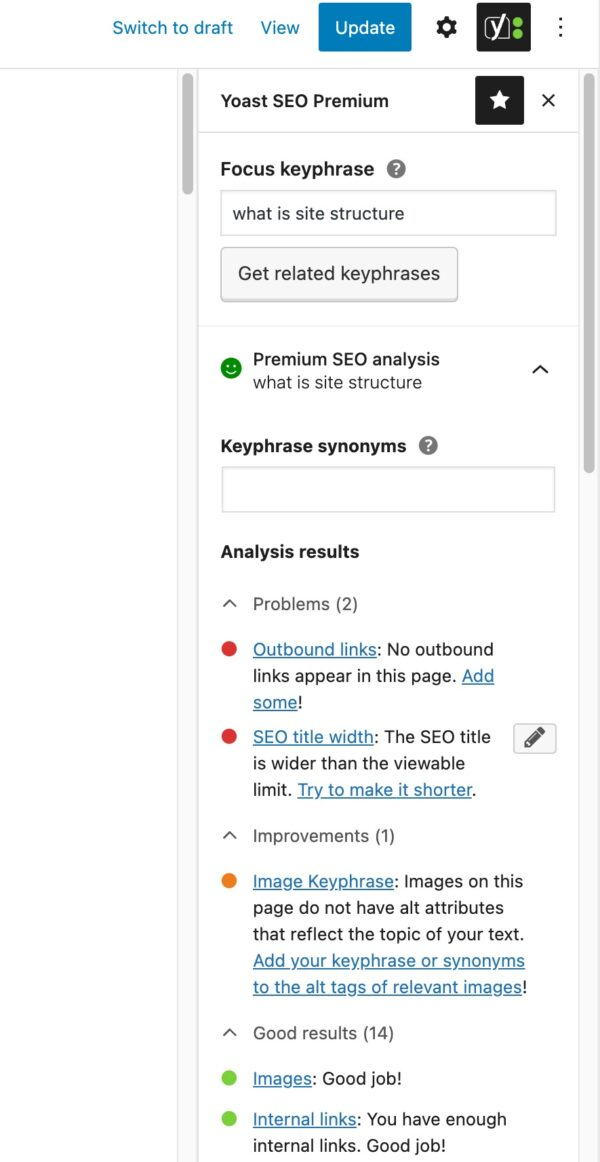
\includegraphics[width=0.4\columnwidth]{soluzioni-esistenti/Yoast-SEO/yoast_seo_premium.png}} 
    \caption{Yoast SEO Premium - Analisi SEO}
    \label{fig:yoast_seo}
\end{figure}

\section{Keyword Density Analyzer}

\subsection{Funzionalità}
\par \textit{Keyword Density Analyzer} è uno strumento di analisi \gls{seo} fornito da \textit{Webmaster Tips}. L'analisi inizia con una panoramica generale della pagina esaminata, che include le seguenti informazioni:
\begin{itemize}
    \item URL, titolo, meta description e lingua;
    \item Dimensione della pagina non compressa;
    \item Dimensione del contenuto di testo semplice;
    \item Rapporto testo semplice/codice \gls{html};
    \item Conteggio di caratteri e parole;
    \item \textbf{Top keywords}: elenco delle parole chiave considerate più rilevanti in base a parametri interni all'applicazione.
\end{itemize}
\vspace{5pt}
\par\noindent Viene poi effettuata un'analisi del titolo e della meta description, evidenziando la frequenza e la densità di ciascuna parola contenuta in questi tag. L'analisi delle parole chiave è suddivisa in quattro sezioni:
\begin{itemize}
    \item \textbf{Meta tag keywords}: mostra la frequenza e la densità delle parole chiave specificate nel meta tag keywords;
    \item \textbf{Top Keywords by Density}: elenca le parole più frequenti, escludendo quelle comuni e troppo brevi. Oltre alla frequenza e alla densità, mostra anche il numero di occorrenze nel titolo, negli heading, nei link e nel testo alternativo delle immagini;
    \item \textbf{Top Keywords by Score}: elenca le parole in base a un punteggio calcolato internamente, come mostrato in figura \ref{fig:keyword_density_analyzer};
    \item \textbf{Top Phrases}: elenca le frasi con più di una occorrenza, escludendo quelle brevi e con parole comuni.
\end{itemize}

\vspace{10pt}
\par\noindent La figura \ref{fig:keyword_density_analyzer_w3schools} mostra un esempio di analisi del sito “W3Schools” effettuata con \textit{Keyword Density Analyzer}.

\begin{figure}[H]
    \centering 
    \fbox{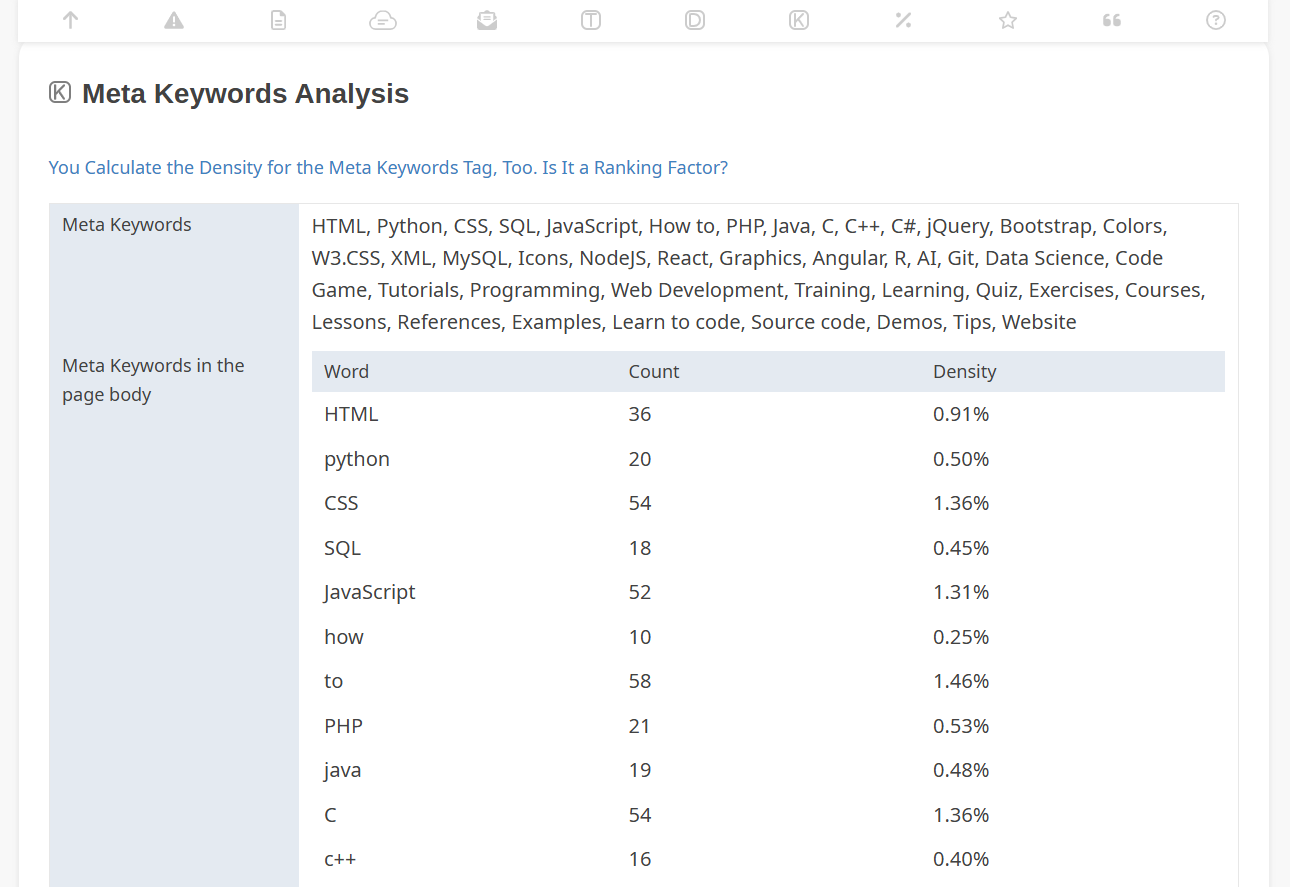
\includegraphics[width=0.8\columnwidth]{soluzioni-esistenti/Keywords-Density-Analyzer/keywords_density_analyzer.png}} 
    \caption{Keyword Density Analyzer - Analisi del sito “W3Schools”}
    \label{fig:keyword_density_analyzer_w3schools}
\end{figure}

\subsection{Vantaggi}
\par Tutte le funzionalità sono gratuite e possono essere integrate con gli altri strumenti di \textit{Webmaster Tips} per un'analisi \gls{seo} completa.

\subsection{Svantaggi}
\par L'analisi di una pagina web richiede di interrompere la navigazione e accedere alla piattaforma di \textit{Webmaster Tips}.

\begin{figure}[H]
    \centering 
    \fbox{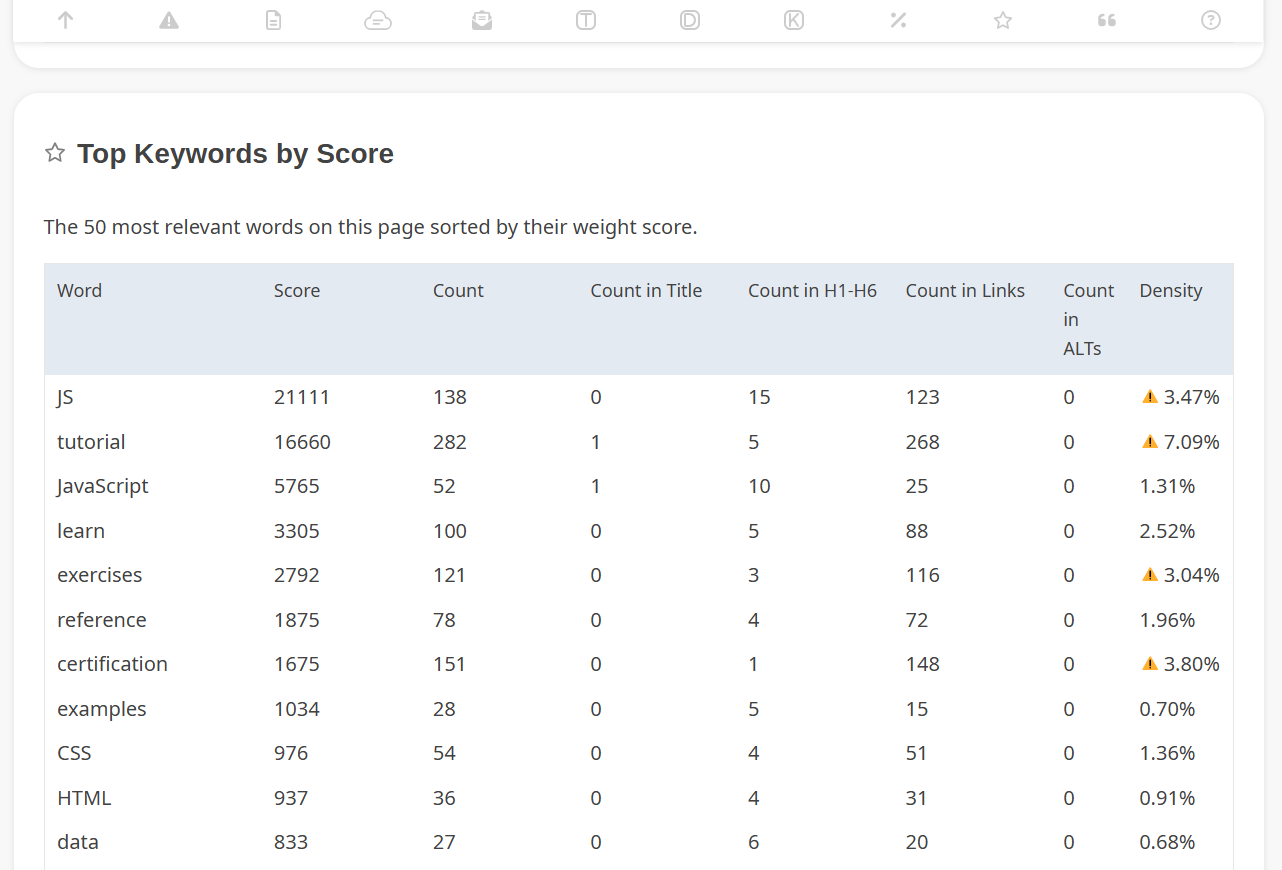
\includegraphics[width=0.8\columnwidth]{soluzioni-esistenti/Keywords-Density-Analyzer/keywords_density_analyzer_score.png}} 
    \caption{Keyword Density Analyzer - Top Keywords by Score}
    \label{fig:keyword_density_analyzer}
\end{figure}

\section{Detailed SEO Extension}

\subsection{Funzionalità}
\par \textit{Detailed SEO Extension} è un'estensione per Google Chrome e Firefox che consente di analizzare, con un solo clic, qualsiasi sito web. L'estensione estrae e analizza i seguenti elementi:
\begin{itemize}
    \item \textbf{Overview}: Titolo, meta description, URL, \gls{tag-canonical}, \gls{tag-robots}, meta tag keywords, numero di parole e lingua;
    \item \textbf{Gerarchia degli heading} (da H1 a H6): l'estensione regola l'indentazione e la dimensione del font in base al livello, facilitando l'analisi visiva della struttura;
    \item \textbf{Link} (unici, interni o esterni, completi o incompleti);
    \item \textbf{Immagini} (complete o prive di attributi);
    \item \textbf{Schema e \gls{hreflang}};
    \item \textbf{Ottimizzazione per i social media}.
\end{itemize}
\vspace{5pt}
\par\noindent Inoltre, l'estensione genera automaticamente i link per analizzare la stessa pagina web su altre piattaforme, tra cui \textit{Ahrefs}, \textit{Majestic}, \textit{Moz}, \textit{Semrush} e \textit{SimilarWeb}. La figura \ref{fig:detailed_seo_extension_w3schools} mostra un esempio di analisi del sito “W3Schools” effettuata con \textit{Detailed SEO Extension}.
 
\begin{figure}[H]
    \centering 
    \fbox{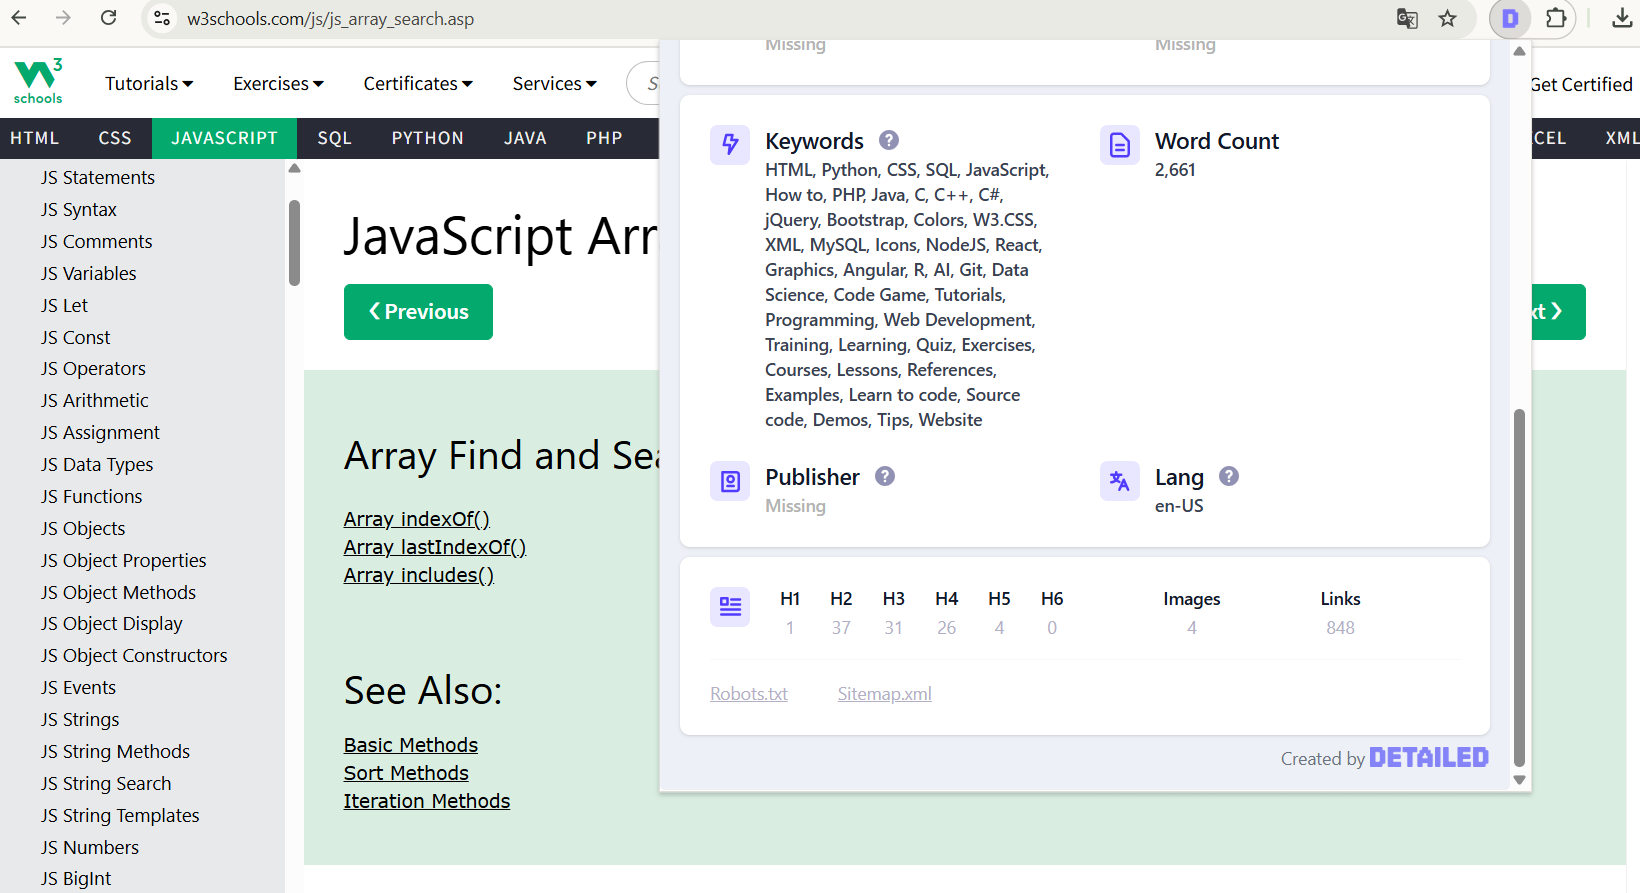
\includegraphics[width=0.8\columnwidth]{soluzioni-esistenti/Detailed-SEO-Extension/detailed_seo_analysis.png}} 
    \caption{Detailed SEO Extension - Analisi del sito “W3Schools”}
    \label{fig:detailed_seo_extension_w3schools}
\end{figure}

\subsection{Vantaggi}
\par Essendo gratuita e compatibile con \gls{localhost}, l'estensione si presta perfettamente all'uso durante la fase di sviluppo.

\subsection{Svantaggi}
\par L'estensione si apre come pop-up, il che può rendere meno agevole l'interazione con la pagina corrente. Per quanto riguarda l'analisi delle parole chiave, lo strumento si limita a estrarre quelle presenti nel meta tag keywords.

\section{SEO Analyzer (Rank Math)}

\subsection{Funzionalità}
\par \textit{Rank Math} è un plugin per \gls{wordpress} che semplifica l'ottimizzazione \gls{seo} mediante suggerimenti basati sulle \textit{best practice}. Lo strumento \textit{SEO Analyzer} esegue un'analisi approfondita delle pagine web, generando un punteggio complessivo. Inoltre, \textit{SEO Analyzer} visualizza un elenco delle parole chiave più frequenti e verifica che siano distribuite correttamente.

\subsection{Vantaggi}
\par \textit{SEO Analyzer} è in grado di analizzare anche siti web che non sono stati realizzati con \gls{wordpress}.

\subsection{Svantaggi}
\par \textit{SEO Analyzer} non funziona su \gls{localhost} ed è meno affidabile rispetto ad altri strumenti, in quanto l'analisi dei tag è \gls{case-sensitive}, il che può portare a errori come il mancato rilevamento della meta description. Inoltre, la versione Premium di \textit{Rank Math} è a pagamento. 

\vspace{10pt}
\par\noindent La figura \ref{fig:rank_math_silktide} mostra un esempio di analisi del sito “Silktide” effettuata con \textit{Rank Math}.

\begin{figure}[H]
    \centering 
    \fbox{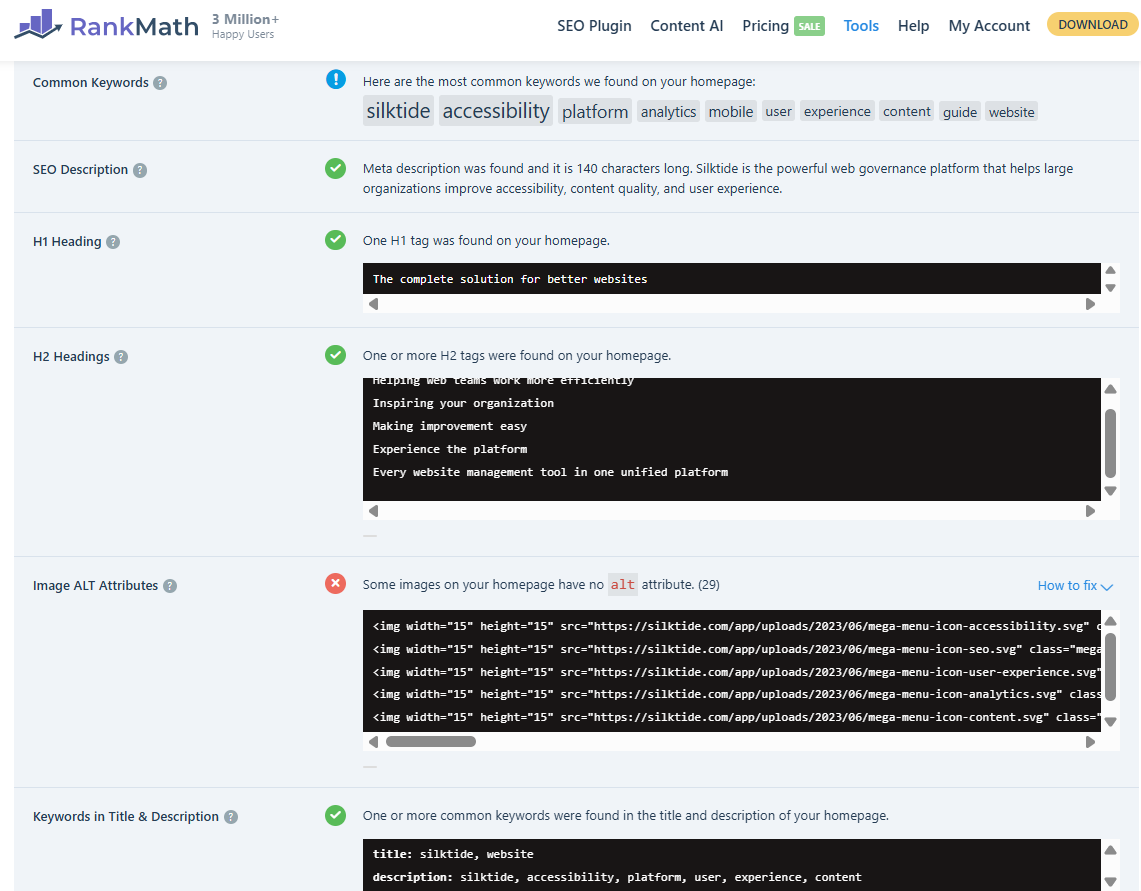
\includegraphics[width=0.7\columnwidth]{soluzioni-esistenti/RankMath/rank_math.png}} 
    \caption{Rank Math - Analisi del sito “Silktide”}
    \label{fig:rank_math_silktide}
\end{figure}
        \chapter{Analisi dei requisiti}
\label{cap:analisi-requisiti}

\intro{In questa sezione sono elencati i requisiti e le user story, attraverso cui vengono descritte e formalizzate le funzionalità dell’applicazione e le esigenze dell’utente finale.}

\section{Introduzione}

\par L'analisi dei \gls{requisiti} è stata condotta seguendo gli standard dell'ingegneria del software, integrando la valutazione delle soluzioni esistenti con colloqui e dialoghi con la Proponente. In questa sezione vengono illustrati i seguenti punti:
\begin{itemize}
    \item \textbf{\Gls{use-case}}: descrizione e diagrammi dei casi d'uso;
    \item \textbf{Tracciamento dei requisiti}: associa ciascun requisito alla sua fonte di provenienza;
    \item \textbf{\Gls{user-story}}: descrizione delle esigenze dell’utente finale.
\end{itemize}

\section{Casi d'uso}

\paragraph*{Attori}
\par L'unico attore coinvolto nell'interazione con il sistema è un \textbf{utente generico} con accesso completo allo strumento di analisi \gls{seo}. Di seguito sono elencate alcune tipologie di utenti a cui è rivolto il progetto:
\begin{itemize}
    \item \textbf{Sviluppatore}: utilizza l'estensione durante lo sviluppo e la produzione di contenuti web;
    \item \textbf{Tester}: effettua un'analisi SEO per identificare eventuali problemi e proporre azioni di miglioramento;
    \item \textbf{Professore}: utilizza l'estensione per analizzare progetti didattici.
\end{itemize}

\begin{figure}[H] 
    \centering 
    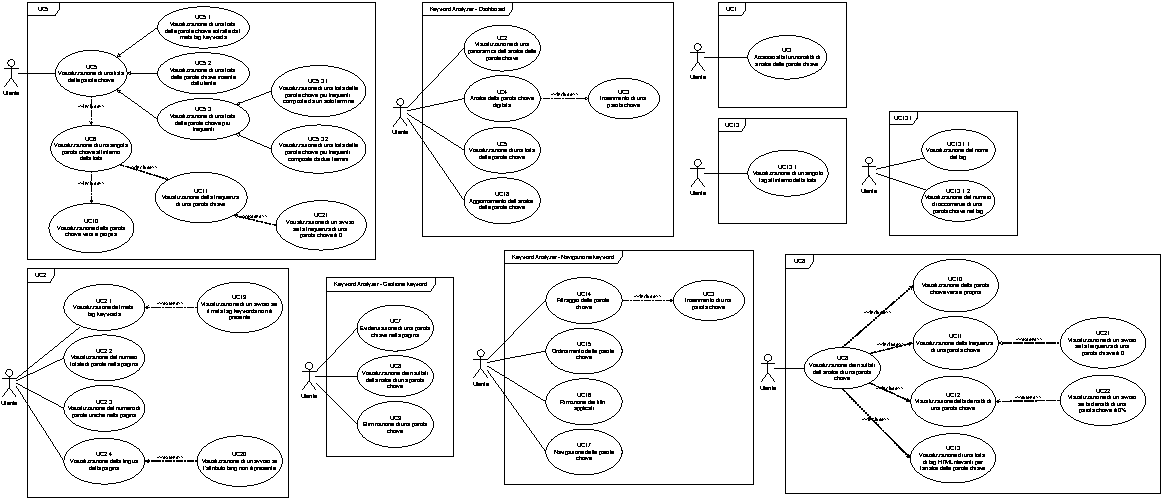
\includegraphics[width=\columnwidth]{usecase/diagrammi_use_case} 
    \caption{Diagrammi dei casi d'uso}
\end{figure}

\begin{usecase}{1}{Accesso allo strumento di analisi delle parole chiave}\label{UC1}
    \usecaseactors{Utente.}
    \usecasepre{L'utente ha avviato l'estensione.}
    \usecasedesc{L'utente seleziona lo strumento di analisi delle parole chiave.}
    \usecasepost{Il sistema mostra la schermata di analisi delle parole chiave.}
\end{usecase}

\begin{usecase}{2}{Visualizzazione di una panoramica dell'analisi delle parole chiave}\label{UC2}
    \usecaseactors{Utente.}
    \usecasepreEnv{\begin{itemize}
        \item L'utente ha selezionato lo strumento di analisi delle parole chiave;
        \item Il sistema è attivo e funzionante.
    \end{itemize}}
    \usecasepost{Il sistema mostra una panoramica dell'analisi delle parole chiave.}
    \usecasesubEnv{\begin{itemize}
        \item \hyperref[UC2point1]{UC2.1}: Visualizzazione del meta tag keywords;
        \item \hyperref[UC2point2]{UC2.2}: Visualizzazione del numero totale di parole nella pagina;
        \item \hyperref[UC2point3]{UC2.3}: Visualizzazione del numero di parole uniche nella pagina;
        \item \hyperref[UC2point4]{UC2.4}: Visualizzazione della lingua della pagina.
    \end{itemize}}
\end{usecase}

\begin{usecase}{2.1}{Visualizzazione del meta tag keywords}\label{UC2point1}
    \usecaseactors{Utente.}
    \usecasepreEnv{\begin{itemize}
        \item L'utente ha selezionato lo strumento di analisi delle parole chiave;
        \item Il sistema è attivo e funzionante.
    \end{itemize}}
    \usecasepost{Il sistema mostra il contenuto del meta tag keywords.}
    \usecaseextEnv{\begin{itemize}
        \item \hyperref[UC19]{UC19}: Visualizzazione di un avviso se il meta tag keywords non è presente.
    \end{itemize}}
\end{usecase}

\begin{usecase}{2.2}{Visualizzazione del numero totale di parole nella pagina}\label{UC2point2}
    \usecaseactors{Utente.}
    \usecasepreEnv{\begin{itemize}
        \item L'utente ha selezionato lo strumento di analisi delle parole chiave;
        \item Il sistema è attivo e funzionante.
    \end{itemize}}
    \usecasepost{Il sistema mostra il numero totale di parole presenti nella pagina.}
\end{usecase}

\begin{usecase}{2.3}{Visualizzazione del numero di parole uniche nella pagina}\label{UC2point3}
    \usecaseactors{Utente.}
    \usecasepreEnv{\begin{itemize}
        \item L'utente ha selezionato lo strumento di analisi delle parole chiave;
        \item Il sistema è attivo e funzionante.
    \end{itemize}}
    \usecasepost{Il sistema mostra il numero di parole uniche presenti nella pagina.}
\end{usecase}

\begin{usecase}{2.4}{Visualizzazione della lingua della pagina}\label{UC2point4}
    \usecaseactors{Utente.}
    \usecasepreEnv{\begin{itemize}
        \item L'utente ha selezionato lo strumento di analisi delle parole chiave;
        \item Il sistema è attivo e funzionante.
    \end{itemize}}
    \usecasepost{Il sistema mostra la lingua dichiarata nella pagina.}
    \usecaseextEnv{\begin{itemize}
        \item \hyperref[UC20]{UC20}: Visualizzazione di un avviso se l'attributo lang non è presente.
    \end{itemize}}
\end{usecase}

\begin{usecase}{3}{Inserimento di una parola chiave}\label{UC3}
    \usecaseactors{Utente.}
    \usecasepreEnv{\begin{itemize}
        \item L'utente ha selezionato lo strumento di analisi delle parole chiave;
        \item Il sistema è attivo e funzionante.
    \end{itemize}}
    \usecasedesc{L'utente digita una parola chiave.}
    \usecasepost{Il sistema mostra la parola chiave inserita dall'utente nell'apposito campo di testo.}
\end{usecase}

\begin{usecase}{4}{Analisi della parola chiave digitata}\label{UC4}
    \usecaseactors{Utente.}
    \usecasepreEnv{\begin{itemize}
        \item L'utente ha selezionato lo strumento di analisi delle parole chiave;
        \item Il sistema è attivo e funzionante;
        \item L'utente ha digitato una parola chiave.
    \end{itemize}}
    \usecasedesc{Il sistema esegue l'analisi della parola chiave digitata dall'utente.}
    \usecasepost{Il sistema aggiunge la parola chiave analizzata alla lista delle keyword.}
    \usecaseincEnv{\begin{itemize}
        \item \hyperref[UC3]{UC3}: Inserimento di una parola chiave.
    \end{itemize}}
\end{usecase}

\begin{usecase}{5}{Visualizzazione di una lista delle parole chiave}\label{UC5}
    \usecaseactors{Utente.}
    \usecasepreEnv{\begin{itemize}
        \item L'utente ha selezionato lo strumento di analisi delle parole chiave;
        \item Il sistema è attivo e funzionante.
    \end{itemize}}
    \usecasepost{Il sistema mostra una lista delle parole chiave.}
    \usecasesubEnv{\begin{itemize}
        \item \hyperref[UC5point1]{UC5.1}: Visualizzazione di una lista delle parole chiave estratte dal meta tag keywords;
        \item \hyperref[UC5point2]{UC5.2}: Visualizzazione di una lista delle parole chiave inserite dall'utente;
        \item \hyperref[UC5point3]{UC5.3}: Visualizzazione di una lista delle parole chiave più frequenti.
    \end{itemize}}
    \usecaseincEnv{\begin{itemize}
        \item \hyperref[UC6]{UC6}: Visualizzazione di una singola parola chiave all’interno della lista.
    \end{itemize}}
\end{usecase}

\begin{usecase}{5.1}{Visualizzazione di una lista delle parole chiave estratte dal meta tag keywords}\label{UC5point1}
    \usecaseactors{Utente.}
    \usecasepreEnv{\begin{itemize}
        \item L'utente ha selezionato lo strumento di analisi delle parole chiave;
        \item Il sistema è attivo e funzionante.
    \end{itemize}}
    \usecasepost{Il sistema mostra una lista delle parole chiave estratte dal meta tag keywords.}
\end{usecase}

\begin{usecase}{5.2}{Visualizzazione di una lista delle parole chiave inserite dall'utente}\label{UC5point2}
    \usecaseactors{Utente.}
    \usecasepreEnv{\begin{itemize}
        \item L'utente ha selezionato lo strumento di analisi delle parole chiave;
        \item Il sistema è attivo e funzionante.
    \end{itemize}}
    \usecasepost{Il sistema mostra una lista delle parole chiave inserite dall'utente.}
\end{usecase}

\begin{usecase}{5.3}{Visualizzazione di una lista delle parole chiave più frequenti}\label{UC5point3}
    \usecaseactors{Utente.}
    \usecasepreEnv{\begin{itemize}
        \item L'utente ha selezionato lo strumento di analisi delle parole chiave;
        \item Il sistema è attivo e funzionante.
    \end{itemize}}
    \usecasepost{Il sistema mostra una lista delle parole chiave più frequenti, estratte automaticamente da un algoritmo interno.}
    \usecasesubEnv{\begin{itemize}
        \item \hyperref[UC5point3point1]{UC5.3.1}: Visualizzazione di una lista delle parole chiave più frequenti composte da un solo termine;
        \item \hyperref[UC5point3point2]{UC5.3.2}: Visualizzazione di una lista delle parole chiave più frequenti composte da due termini.
    \end{itemize}}
\end{usecase}

\begin{usecase}{5.3.1}{Visualizzazione di una lista delle parole chiave più frequenti composte da un solo termine}\label{UC5point3point1}
    \usecaseactors{Utente.}
    \usecasepreEnv{\begin{itemize}
        \item L'utente ha selezionato lo strumento di analisi delle parole chiave;
        \item Il sistema è attivo e funzionante.
    \end{itemize}}
    \usecasepost{Il sistema mostra una lista delle parole chiave più frequenti composte da un solo termine (keyword semplici).}
\end{usecase}

\begin{usecase}{5.3.2}{Visualizzazione di una lista delle parole chiave più frequenti composte da due termini}\label{UC5point3point2}
    \usecaseactors{Utente.}
    \usecasepreEnv{\begin{itemize}
        \item L'utente ha selezionato lo strumento di analisi delle parole chiave;
        \item Il sistema è attivo e funzionante.
    \end{itemize}}
    \usecasepost{Il sistema mostra una lista delle parole chiave più frequenti composte da due termini (keyphrase).}
\end{usecase}

\begin{usecase}{6}{Visualizzazione di una singola parola chiave all’interno della lista}\label{UC6}
    \usecaseactors{Utente.}
    \usecasepreEnv{\begin{itemize}
        \item L'utente ha selezionato lo strumento di analisi delle parole chiave;
        \item Il sistema è attivo e funzionante;
        \item È visibile la lista delle parole chiave.
    \end{itemize}}
    \usecasepost{L'utente visualizza una singola parola chiave all’interno della lista.}
    \usecaseincEnv{\begin{itemize}
        \item \hyperref[UC10]{UC10}: Visualizzazione della parola chiave vera e propria;
        \item \hyperref[UC11]{UC11}: Visualizzazione della frequenza di una parola chiave.
    \end{itemize}}
\end{usecase}

\begin{usecase}{7}{Evidenziazione di una parola chiave nella pagina}\label{UC7}
    \usecaseactors{Utente.}
    \usecasepreEnv{\begin{itemize}
        \item L'utente ha selezionato lo strumento di analisi delle parole chiave;
        \item Il sistema è attivo e funzionante.
    \end{itemize}}
    \usecasepost{Il sistema evidenzia graficamente tutte le occorrenze di una parola chiave nella pagina.}
\end{usecase}

\begin{usecase}{8}{Visualizzazione dei risultati dell'analisi di una parola chiave}\label{UC8}
    \usecaseactors{Utente.}
    \usecasepreEnv{\begin{itemize}
        \item L'utente ha selezionato lo strumento di analisi delle parole chiave;
        \item Il sistema è attivo e funzionante.
    \end{itemize}}
    \usecasepost{L'utente visualizza i risultati dell'analisi di una parola chiave.}
    \usecaseincEnv{\begin{itemize}
        \item \hyperref[UC10]{UC10}: Visualizzazione della parola chiave vera e propria;
        \item \hyperref[UC11]{UC11}: Visualizzazione della frequenza di una parola chiave;
        \item \hyperref[UC12]{UC12}: Visualizzazione della densità di una parola chiave;
        \item \hyperref[UC13]{UC13}: Visualizzazione di una lista di tag \gls{html} rilevanti per l’analisi delle parole chiave.
    \end{itemize}}
\end{usecase}

\begin{usecase}{9}{Eliminazione di una parola chiave}\label{UC9}
    \usecaseactors{Utente.}
    \usecasepreEnv{\begin{itemize}
        \item L'utente ha selezionato lo strumento di analisi delle parole chiave;
        \item Il sistema è attivo e funzionante.
    \end{itemize}}
    \usecasedesc{L'utente elimina una parola chiave.}
    \usecasepost{Il sistema rimuove la parola chiave dalla lista delle keyword.}
\end{usecase}

\begin{usecase}{10}{Visualizzazione della parola chiave vera e propria}\label{UC10}
    \usecaseactors{Utente.}
    \usecasepreEnv{\begin{itemize}
        \item L'utente ha selezionato lo strumento di analisi delle parole chiave;
        \item Il sistema è attivo e funzionante.
    \end{itemize}}
    \usecasepost{L’utente visualizza la parola chiave vera e propria (es. “JavaScript”).}
\end{usecase}

\begin{usecase}{11}{Visualizzazione della frequenza di una parola chiave}\label{UC11}
    \usecaseactors{Utente.}
    \usecasepreEnv{\begin{itemize}
        \item L'utente ha selezionato lo strumento di analisi delle parole chiave;
        \item Il sistema è attivo e funzionante.
    \end{itemize}}
    \usecasepost{L'utente visualizza la frequenza di una parola chiave.}
    \usecaseextEnv{\begin{itemize}
        \item \hyperref[UC19]{UC19}: Visualizzazione di un avviso se la frequenza di una parola chiave è 0.
    \end{itemize}}
\end{usecase}

\begin{usecase}{12}{Visualizzazione della densità di una parola chiave}\label{UC12}
    \usecaseactors{Utente.}
    \usecasepreEnv{\begin{itemize}
        \item L'utente ha selezionato lo strumento di analisi delle parole chiave;
        \item Il sistema è attivo e funzionante.
    \end{itemize}}
    \usecasepost{L'utente visualizza la densità percentuale di una parola chiave.}
    \usecaseextEnv{\begin{itemize}
        \item \hyperref[UC20]{UC20}: Visualizzazione di un avviso se la densità di una parola chiave è 0\%.
    \end{itemize}}
\end{usecase}

\begin{usecase}{13}{Visualizzazione di una lista di tag HTML rilevanti per l’analisi delle parole chiave}\label{UC13}
    \usecaseactors{Utente.}
    \usecasepreEnv{\begin{itemize}
        \item L'utente ha selezionato lo strumento di analisi delle parole chiave;
        \item Il sistema è attivo e funzionante.
    \end{itemize}}
    \usecasepost{L’utente visualizza una lista di tag \gls{html} considerati rilevanti per l’analisi delle parole chiave.}
    \usecasesubEnv{\begin{itemize}
        \item \hyperref[UC13point1]{UC13.1}: Visualizzazione di un singolo tag all’interno della lista.
    \end{itemize}}
\end{usecase}

\begin{usecase}{13.1}{Visualizzazione di un singolo tag all’interno della lista}\label{UC13point1}
    \usecaseactors{Utente.}
    \usecasepreEnv{\begin{itemize}
        \item L'utente ha selezionato lo strumento di analisi delle parole chiave;
        \item Il sistema è attivo e funzionante;
        \item L'utente sta visualizzando i risultati dell'analisi di una parola chiave;
        \item È visibile l'elenco dei tag \gls{html}.
    \end{itemize}}
    \usecasepost{L'utente visualizza un singolo tag all’interno della lista.}
    \usecasesubEnv{\begin{itemize}
        \item \hyperref[UC13point1point1]{UC13.1.1}: Visualizzazione del nome del tag;
        \item \hyperref[UC13point1point2]{UC13.1.2}: Visualizzazione del numero di occorrenze di una parola chiave nel tag.
    \end{itemize}}
\end{usecase}

\begin{usecase}{13.1.1}{Visualizzazione del nome del tag}\label{UC13point1point1}
    \usecaseactors{Utente.}
    \usecasepreEnv{\begin{itemize}
        \item L'utente ha selezionato lo strumento di analisi delle parole chiave;
        \item Il sistema è attivo e funzionante.
    \end{itemize}}
    \usecasepost{L'utente visualizza il nome del tag \gls{html}.}
\end{usecase}

\begin{usecase}{13.1.2}{Visualizzazione del numero di occorrenze di una parola chiave nel tag}\label{UC13point1point2}
    \usecaseactors{Utente.}
    \usecasepreEnv{\begin{itemize}
        \item L'utente ha selezionato lo strumento di analisi delle parole chiave;
        \item Il sistema è attivo e funzionante.
    \end{itemize}}
    \usecasepost{L'utente visualizza il numero di occorrenze di una parola chiave nel tag \gls{html}.}
\end{usecase}

\begin{usecase}{14}{Filtraggio delle parole chiave}\label{UC14}
    \usecaseactors{Utente.}
    \usecasepreEnv{\begin{itemize}
        \item L'utente ha selezionato lo strumento di analisi delle parole chiave;
        \item Il sistema è attivo e funzionante.
    \end{itemize}}
    \usecasepost{Il sistema filtra le parole chiave per nome.}
    \usecaseincEnv{\begin{itemize}
        \item \hyperref[UC3]{UC3}: Inserimento di una parola chiave.
    \end{itemize}}
\end{usecase}

\begin{usecase}{15}{Ordinamento delle parole chiave}\label{UC15}
    \usecaseactors{Utente.}
    \usecasepreEnv{\begin{itemize}
        \item L'utente ha selezionato lo strumento di analisi delle parole chiave;
        \item Il sistema è attivo e funzionante.
    \end{itemize}}
    \usecasepost{Il sistema ordina le parole chiave per frequenza crescente o decrescente.}
\end{usecase}

\begin{usecase}{16}{Rimozione dei filtri applicati}\label{UC16}
    \usecaseactors{Utente.}
    \usecasepreEnv{\begin{itemize}
        \item L'utente ha selezionato lo strumento di analisi delle parole chiave;
        \item Il sistema è attivo e funzionante.
    \end{itemize}}
    \usecasepost{L’utente rimuove i filtri applicati alle parole chiave.}
\end{usecase}

\begin{usecase}{17}{Navigazione delle parole chiave}\label{UC17}
    \usecaseactors{Utente.}
    \usecasepreEnv{\begin{itemize}
        \item L'utente ha selezionato lo strumento di analisi delle parole chiave;
        \item Il sistema è attivo e funzionante.
    \end{itemize}}
    \usecasepost{L’utente naviga tra le parole chiave tramite un sistema di paginazione.}
\end{usecase}

\begin{usecase}{18}{Aggiornamento dell'analisi delle parole chiave}\label{UC18}
    \usecaseactors{Utente.}
    \usecasepreEnv{\begin{itemize}
        \item L'utente ha selezionato lo strumento di analisi delle parole chiave;
        \item Il sistema è attivo e funzionante.
    \end{itemize}}
    \usecasedesc{L'utente aggiorna manualmente l'analisi delle parole chiave per sincronizzarla con eventuali modifiche dinamiche al \gls{dom}.}
    \usecasepost{Il sistema aggiorna l'analisi delle parole chiave.}
\end{usecase}

\begin{usecase}{19}{Visualizzazione di un avviso se il meta tag keywords non è presente}\label{UC19}
    \usecaseactors{Utente.}
    \usecasepreEnv{\begin{itemize}
        \item L'utente ha selezionato lo strumento di analisi delle parole chiave;
        \item Il sistema è attivo e funzionante;
        \item Il meta tag keywords non è presente nella pagina analizzata.
    \end{itemize}}
    \usecasepost{Il sistema mostra un avviso in cui notifica all'utente che il meta tag keywords non è presente.}
\end{usecase}

\begin{usecase}{20}{Visualizzazione di un avviso se l’attributo lang non è presente}\label{UC20}
    \usecaseactors{Utente.}
    \usecasepreEnv{\begin{itemize}
        \item L'utente ha selezionato lo strumento di analisi delle parole chiave;
        \item Il sistema è attivo e funzionante;
        \item Il tag <html> non contiene l’attributo lang.
    \end{itemize}}
    \usecasepost{Il sistema mostra un avviso in cui notifica all'utente che l'attributo lang non è presente.}
\end{usecase}

\begin{usecase}{21}{Visualizzazione di un avviso se la frequenza di una parola chiave è 0}\label{UC21}
    \usecaseactors{Utente.}
    \usecasepreEnv{\begin{itemize}
        \item L'utente ha selezionato lo strumento di analisi delle parole chiave;
        \item Il sistema è attivo e funzionante;
        \item La frequenza di una parola chiave è 0.
    \end{itemize}}
    \usecasepost{Il sistema mostra un avviso in cui notifica all'utente che la frequenza di una parola chiave è 0.}
\end{usecase}

\begin{usecase}{22}{Visualizzazione di un avviso se la densità di una parola chiave è 0\%}\label{UC22}
    \usecaseactors{Utente.}
    \usecasepreEnv{\begin{itemize}
        \item L'utente ha selezionato lo strumento di analisi delle parole chiave;
        \item Il sistema è attivo e funzionante;
        \item La densità di una parola chiave è 0\%.
    \end{itemize}}
    \usecasepost{Il sistema mostra un avviso in cui notifica all'utente che la densità di una parola chiave è 0\%.}
\end{usecase}

\begin{usecase}{23}{Aggiornamento del colore di evidenziazione per un tag HTML}\label{UC23}
    \usecaseactors{Utente.}
    \usecasepreEnv{\begin{itemize}
        \item L'utente ha selezionato lo strumento di analisi delle parole chiave;
        \item Il sistema è attivo e funzionante.
    \end{itemize}}
    \usecasepost{L'utente personalizza il colore con cui vengono evidenziate le occorrenze di una parola chiave all’interno di uno specifico tag \gls{html}.}
    \usecasesubEnv{\begin{itemize}
        \item \hyperref[UC23point1]{UC23.1}: Aggiornamento del colore di sfondo;
        \item \hyperref[UC23point2]{UC23.2}: Aggiornamento del colore del testo;
        \item \hyperref[UC23point3]{UC23.3}: Aggiornamento del colore del bordo.
    \end{itemize}}
\end{usecase}

\begin{usecase}{23.1}{Aggiornamento del colore di sfondo}\label{UC23point1}
    \usecaseactors{Utente.}
    \usecasepreEnv{\begin{itemize}
        \item L'utente ha selezionato lo strumento di analisi delle parole chiave;
        \item Il sistema è attivo e funzionante.
    \end{itemize}}
    \usecasepost{L'utente personalizza il colore di sfondo con cui vengono evidenziate le occorrenze di una parola chiave all’interno di uno specifico tag \gls{html}.}
\end{usecase}

\begin{usecase}{23.2}{Aggiornamento del colore del testo}\label{UC23point2}
    \usecaseactors{Utente.}
    \usecasepreEnv{\begin{itemize}
        \item L'utente ha selezionato lo strumento di analisi delle parole chiave;
        \item Il sistema è attivo e funzionante.
    \end{itemize}}
    \usecasepost{L'utente personalizza il colore del testo con cui vengono evidenziate le occorrenze di una parola chiave all’interno di uno specifico tag \gls{html}.}
\end{usecase}

\begin{usecase}{23.3}{Aggiornamento del colore del bordo}\label{UC23point3}
    \usecaseactors{Utente.}
    \usecasepreEnv{\begin{itemize}
        \item L'utente ha selezionato lo strumento di analisi delle parole chiave;
        \item Il sistema è attivo e funzionante.
    \end{itemize}}
    \usecasepost{L'utente personalizza il colore del bordo con cui vengono evidenziate le occorrenze di una parola chiave all’interno di uno specifico tag \gls{html}.}
\end{usecase}

\newpage

\section{Tracciamento dei requisiti}
\par I \gls{requisiti} del progetto, individuati e formalizzati durante il processo di analisi, sono illustrati nelle tabelle \ref{tab:requisiti-funzionali}, \ref{tab:requisiti-qualitativi} e \ref{tab:requisiti-vincolo} secondo la seguente notazione:
\par \textbf{\[R[Tipologia].[Importanza].[Codice]\]} 
\par dove:
\par\vspace{20pt}
\begin{tabular}{@{}ll@{}}
    R = & requisito \\
    \textbf{Tipologia}: & \\
    \quad F = & funzionale \\
    \quad Q = & di qualità \\
    \quad V = & di vincolo/dominio \\
    \textbf{Importanza}: & \\
    \quad O = & obbligatorio \\
    \quad D = & desiderabile \\  
    \quad OP = & opzionale \\
    Codice = & codice numerico univoco \\
\end{tabular}
    
\par\vspace{30pt}

\renewcommand{\arraystretch}{1.5}
\begin{tabularx}{\textwidth}{l >{\raggedright\arraybackslash}X l}
\caption{Tabella dei requisti funzionali}
\label{tab:requisiti-funzionali} \\
\hline\hline
\textbf{Requisito} & \textbf{Descrizione} & \textbf{Fonti} \\
\endfirsthead

\caption[]{Tabella dei requisiti funzionali (continua)} \\
\hline\hline
\textbf{Requisito} & \textbf{Descrizione} & \textbf{Fonti} \\ 
\endhead

\multicolumn{3}{r}{{Continua nella prossima pagina}} \\ 
\endfoot

\hline
\endlastfoot

\hline
RF.O.1 & L'utente deve poter accedere allo strumento di analisi delle parole chiave. & \hyperref[UC1]{UC1} \\
\hline
RF.O.2 & L'utente deve poter visualizzare una panoramica dell'analisi delle parole chiave. & \hyperref[UC2]{UC2} \\
\hline
RF.O.3 & L'utente deve poter visualizzare il contenuto del meta tag keywords. & \hyperref[UC2point1]{UC2.1} \\
\hline
RF.O.4 & L'utente deve poter visualizzare il numero totale di parole nella pagina. & \hyperref[UC2point2]{UC2.2} \\
\hline
RF.D.5 & L'utente deve poter visualizzare il numero di parole uniche nella pagina. & \hyperref[UC2point3]{UC2.3} \\
\hline
RF.O.6 & L'utente deve poter visualizzare la lingua della pagina. & \hyperref[UC2point4]{UC2.4} \\
\hline
RF.O.7 & L'utente deve poter digitare una parola chiave. & \hyperref[UC3]{UC3} \\
\hline
RF.O.8 & L'utente deve poter analizzare la parola chiave digitata. & \hyperref[UC4]{UC4} \\
\hline
RF.O.9 & L'utente deve poter visualizzare una lista delle parole chiave. & \hyperref[UC5]{UC5} \\
\hline
RF.O.10 & L'utente deve poter visualizzare una lista delle parole chiave estratte dal meta tag keywords. & \hyperref[UC5point1]{UC5.1} \\
\hline
RF.O.11 & Il sistema deve visualizzare una lista delle parole chiave inserite dall'utente. & \hyperref[UC5point2]{UC5.2} \\
\hline
RF.OP.12 & L'utente deve poter visualizzare una lista delle parole chiave più frequenti. & \hyperref[UC5point3]{UC5.3} \\
\hline
RF.OP.13 & L'utente deve poter visualizzare una lista delle parole chiave più frequenti composte da un solo termine. & \hyperref[UC5point3point1]{UC5.3.1} \\
\hline
RF.OP.14 & L'utente deve poter visualizzare una lista delle parole chiave più frequenti composte da due termini. & \hyperref[UC5point3point2]{UC5.3.2} \\
\hline
RF.O.15 & L'utente deve poter visualizzare una singola parola chiave all'interno della lista. & \hyperref[UC6]{UC6} \\
\hline
RF.O.16 & Il sistema deve evidenziare tutte le occorrenze di una parola chiave nella pagina. & \hyperref[UC7]{UC7} \\
\hline
RF.O.17 & L'utente deve poter visualizzare i risultati dell'analisi di una parola chiave. & \hyperref[UC8]{UC8} \\
\hline
RF.D.18 & L'utente deve poter eliminare una parola chiave. & \hyperref[UC9]{UC9} \\
\hline
RF.O.19 & L'utente deve poter visualizzare la parola chiave vera e propria (es. “JavaScript”). & \hyperref[UC10]{UC10} \\
\hline
RF.O.20 & L'utente deve poter visualizzare la frequenza di una parola chiave. & \hyperref[UC11]{UC11} \\
\hline
RF.O.21 & L'utente deve poter visualizzare la densità di una parola chiave. & \hyperref[UC12]{UC12} \\
\hline
RF.O.22 & Il sistema deve mostrare una lista di tag \gls{html} rilevanti per l’analisi delle parole chiave. & \hyperref[UC13]{UC13} \\
\hline
RF.O.23 & L'utente deve poter visualizzare un singolo tag all'interno della lista. & \hyperref[UC13point1]{UC13.1} \\
\hline
RF.O.24 & L'utente deve poter visualizzare il nome del tag. & \hyperref[UC13point1point1]{UC13.1.1} \\
\hline
RF.O.25 & L'utente deve poter visualizzare il numero di occorrenze di una parola chiave nel tag. & \hyperref[UC13point1point2]{UC13.1.2} \\
\hline
RF.D.26 & L'utente deve poter filtrare le parole chiave per nome. & \hyperref[UC14]{UC14} \\
\hline
RF.D.27 & L'utente deve poter ordinare le parole chiave per frequenza. & \hyperref[UC15]{UC15} \\
\hline
RF.D.28 & L'utente deve poter rimuovere i filtri applicati alle parole chiave. & \hyperref[UC16]{UC16} \\
\hline
RF.O.29 & L'utente deve poter navigare tra le parole chiave tramite un sistema di paginazione. & \hyperref[UC17]{UC17} \\
\hline
RF.OP.30 & L'utente deve poter aggiornare l'analisi delle parole chiave. & \hyperref[UC18]{UC18} \\
\hline
RF.O.31 & Il sistema deve mostrare un avviso se il meta tag keywords non è presente. & \hyperref[UC19]{UC19} \\
\hline
RF.O.32 & Il sistema deve mostrare un avviso se il tag <html> non contiene l’attributo lang. & \hyperref[UC20]{UC20} \\
\hline
RF.O.33 & Il sistema deve mostrare un avviso se la frequenza di una parola chiave è 0. & \hyperref[UC21]{UC21} \\
\hline
RF.O.34 & Il sistema deve mostrare un avviso se la densità di una parola chiave è 0\%. & \hyperref[UC22]{UC22} \\
\hline
RF.OP.35 & L'utente deve poter aggiornare il colore di evidenziazione per un tag HTML. & \hyperref[UC23]{UC23} \\
\hline
RF.OP.36 & L'utente deve poter personalizzare il colore di sfondo. & \hyperref[UC23point1]{UC23.1} \\
\hline
RF.OP.37 & L'utente deve poter personalizzare il colore del testo. & \hyperref[UC23point2]{UC23.2} \\
\hline
RF.OP.38 & L'utente deve poter personalizzare il colore del bordo. & \hyperref[UC23point3]{UC23.3} \\
\hline
RF.O.39 & Il sistema deve analizzare automaticamente le parole chiave specificate nel meta tag keywords. & DP\textsuperscript{*} \\
\hline
RF.OP.40 & Il sistema deve analizzare automaticamente le parole chiave più frequenti estratte dalla pagina. & DP\textsuperscript{*} \\
\hline
RF.O.41 & Il sistema deve evidenziare le parole chiave con colori diversi in base al tag HTML che le racchiude. & DP\textsuperscript{*} \\
\hline
RF.OP.42 & Il sistema deve escludere le \gls{stopword} durante l'analisi del testo, in modo coerente con la lingua dichiarata nella pagina. & DP\textsuperscript{*} \\
\hline
RF.D.43 & Il sistema deve identificare le keyphrase “spezzate” su più tag HTML. & DP\textsuperscript{*} \\
\end{tabularx}

\vspace{3pt}
\noindent\textsuperscript{*}~DP = Discussione con la Proponente.

\renewcommand{\arraystretch}{1.5}
\begin{tabularx}{\textwidth}{l >{\raggedright\arraybackslash}X l}
\caption{Tabella dei requisti di qualità}
\label{tab:requisiti-qualitativi} \\
\hline\hline
\textbf{Requisito} & \textbf{Descrizione} & \textbf{Fonti}\\
\endfirsthead
    
\caption[]{Tabella dei requisiti di qualità (continua)} \\
\hline\hline
\textbf{Requisito} & \textbf{Descrizione} & \textbf{Fonti} \\ 
\endhead
    
\multicolumn{3}{r}{{Continua nella prossima pagina}} \\ 
\endfoot
    
\hline
\endlastfoot

\hline
RQ.O.1 & Le funzionalità di analisi \gls{seo} devono rispettare le linee guida \gls{wcag} 2.2, livello AA. & DP\textsuperscript{*} \\
\hline
RQ.OP.2 & L'estensione deve rimanere attiva su tutte le tab. & DP\textsuperscript{*} \\
\hline
RQ.D.3 & L'utente deve poter aprire e chiudere l'estensione in modo rapido e intuitivo. & DP\textsuperscript{*} \\
\end{tabularx}

\vspace{3pt}
\noindent\textsuperscript{*}~DP = Discussione con la Proponente.

\renewcommand{\arraystretch}{1.5}
\begin{tabularx}{\textwidth}{l >{\raggedright\arraybackslash}X l}
\caption{Tabella dei requisti di vincolo/dominio}
\label{tab:requisiti-vincolo} \\
\hline\hline
\textbf{Requisito} & \textbf{Descrizione} & \textbf{Fonti}\\
\endfirsthead
        
\caption[]{Tabella dei requisiti di vincolo/dominio (continua)} \\
\hline\hline
\textbf{Requisito} & \textbf{Descrizione} & \textbf{Fonti} \\ 
\endhead
        
\multicolumn{3}{r}{{Continua nella prossima pagina}} \\ 
\endfoot
        
\hline
\endlastfoot

\hline
RV.O.1 & Lo strumento di analisi \gls{seo} deve essere reso disponibile tramite \gls{github} (come codice sorgente) o pubblicato su un'altra piattaforma ad accesso pubblico. & DP\textsuperscript{*} \\
\hline
RV.O.2 & Lo strumento di analisi SEO deve essere integrato all'interno di un'estensione per Chrome. & DP\textsuperscript{*} \\
\end{tabularx}

\vspace{3pt}
\noindent\textsuperscript{*}~DP = Discussione con la Proponente.

\par\vspace{20pt}

\subsection{Riepilogo}

\begin{table}[H]
\centering
\caption{Tabella di riepilogo dei requisiti}
\label{tab:riepilogo-requisiti}
% MAX 12.5cm
\begin{tabular}{ccccc}
\hline\hline
\textbf{Requisito} & \textbf{Obbligatorio} & \textbf{Desiderabile} & \textbf{Opzionale} & \textbf{Totale} \\ 
\hline
Funzionale & 27 & 6 & 10 & 43 \\
\hline
Di qualità & 1 & 1 & 1 & 3 \\
\hline 
Di vincolo/dominio & 2 & 0 & 0 & 2 \\
\hline
\textbf{Totale} & 30 & 7 & 11 & \textbf{48} \\ 
\hline
\end{tabular}
\end{table}

\newpage

\section{User story}

\renewcommand{\arraystretch}{1.5}
\begin{tabularx}{\textwidth}{lX}
\caption{Tabella delle user story}
\label{tab:user-story} \\
\hline\hline
\textbf{ID} & \textbf{User story}\\
\endfirsthead
    
\caption[]{Tabella delle user story (continua)} \\
\hline\hline
\textbf{ID} & \textbf{User story} \\ 
\endhead
    
\multicolumn{2}{r}{{Continua nella prossima pagina}} \\ 
\endfoot
    
\hline
\endlastfoot

\hline
1 & Come utente, voglio visualizzare una panoramica dell'analisi delle parole chiave, in modo da avere un'idea generale del contenuto della pagina. \\
\hline
2 & Come utente, voglio visualizzare il contenuto del meta tag keywords, in modo da verificare se sono state specificate delle parole chiave. \\
\hline
3 & Come utente, voglio visualizzare il numero di parole totali e uniche presenti nella pagina, in modo da valutare la qualità del contenuto. \\
\hline
4 & Come utente, voglio inserire manualmente una parola chiave, in modo da analizzare anche quelle non presenti nel meta tag keywords o non rilevate automaticamente dal sistema. \\
\hline
5 & Come utente, voglio visualizzare un elenco delle parole chiave analizzate, suddivise per categoria, in modo da facilitarne la consultazione. \\
\hline
6 & Come utente, voglio visualizzare graficamente tutte le occorrenze di una parola chiave nella pagina, con colori diversi in base al tag \gls{html} che le contiene, in modo da valutarne la distribuzione. \\
\hline
7 & Come utente, voglio visualizzare i risultati dell’analisi di una parola chiave in una sezione dedicata, in modo da potermi concentrare su una singola keyword alla volta. \\
\hline
8 & Come utente, voglio eliminare una parola chiave, in modo da mantenere pulita la lista delle keyword. \\
\hline
9 & Come utente, voglio visualizzare la frequenza e la densità di una parola chiave, in modo da capire se il suo utilizzo è eccessivo o appropriato. \\
\hline
10 & Come utente, voglio visualizzare il numero di occorrenze di una parola chiave nei principali tag HTML, in modo da capire se è presente nei punti strategici della pagina. \\
\hline
11 & Come utente, voglio filtrare le parole chiave per nome, in modo da individuare più facilmente quelle di mio interesse. \\
\hline
12 & Come utente, voglio ordinare le parole chiave per frequenza, in modo da semplificare l’accesso a quelle più o meno ricorrenti. \\
\hline
13 & Come utente, voglio rimuovere i filtri applicati, in modo da ripristinare la lista delle parole chiave. \\
\hline
14 & Come utente, voglio navigare tra le parole chiave mediante un sistema di paginazione, in modo da scorrere facilmente l’intera lista. \\
\hline
15 & Come utente, voglio aggiornare l'analisi delle parole chiave, in modo da sincronizzarla con eventuali modifiche dinamiche al \gls{dom}. \\
\hline
16 & Come utente, voglio personalizzare i colori di sfondo, testo e bordo associati a un tag HTML, in modo da adattare l'evidenziazione delle parole chiave alle mie esigenze visive. \\
\hline
17 & Come utente, voglio analizzare anche le parole chiave “spezzate” su più tag HTML, in modo da gestire correttamente le keyphrase. \\
\hline
18 & Come utente, voglio che lo strumento di analisi \gls{seo} sia accessibile a tutti. \\
\end{tabularx}
        \chapter{Progettazione e codifica}
\label{cap:progettazione-codifica}

\section{Struttura dell'estensione}
\label{sec:struttura-estensione}

Come rappresentato in figura \ref{fig:struttura_estensione}, l’estensione si basa su tre componenti fondamentali: \textit{manifest.json}, \textit{service worker} \textit{(background script)} e \textit{content script}.

\subsection{Manifest.json}

Il file \textit{manifest.json} è il cuore dell’estensione: descrive il contenuto in un formato strutturato e definisce le regole per l'iniezione dei \textit{content script}.

\subsection{Service Worker}

Il \textit{service worker} è uno script \textit{singleton} che il browser esegue in background. Non ha accesso diretto alle pagine web, ma può interagire con esse tramite i \textit{content script}. Viene utilizzato per gestire gli eventi del browser (come la chiusura di una scheda o il clic sull’icona dell’estensione nella barra degli strumenti) e coordinare i componenti dell'estensione.

\subsection{Content Script}

I \textit{content script} sono file che vengono iniettati nelle pagine web ed eseguiti nel contesto di quelle stesse pagine. Possono visualizzare e manipolare il \gls{dom} in modo analogo agli script caricati da ciascuna pagina. Hanno accesso a un insieme limitato delle \gls{api} di WebExtension, che può essere esteso tramite la comunicazione con i \textit{background script}.

\begin{figure}[H]
  \centering 
  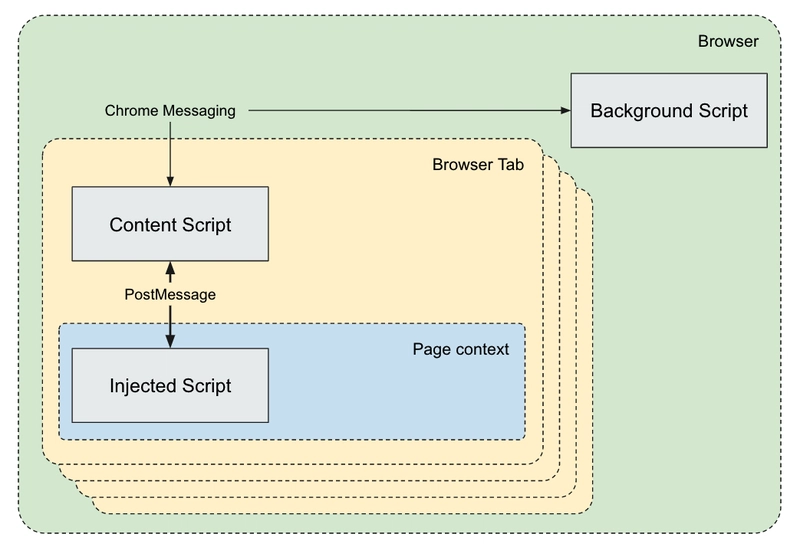
\includegraphics[width=0.8\columnwidth]{progettazione/estensione.png}
  \caption{Struttura dell'estensione}
  \label{fig:struttura_estensione}
\end{figure}

\section{Mockup dell'interfaccia grafica}
\label{sec:mockup}

Durante la progettazione dell’interfaccia grafica, ho tratto ispirazione da diverse soluzioni esistenti analizzate nella fase preliminare. In particolare:
\begin{itemize}
    \item Lo stile delle informazioni in anteprima (come meta keywords, conteggio delle parole e altri dati SEO) si ispira al layout dell’estensione \textit{Detailed SEO Extension}, al quale è stato aggiunto un comportamento flessibile per gestire dinamicamente lo spazio nella barra laterale;
    \item Il \textit{box} di inserimento della parola chiave è il risultato di una combinazione tra le interfacce di \textit{MozBar} e \textit{Wincher}. Da \textit{MozBar} ho ripreso l’idea della \textit{checkbox} posizionata sotto il campo di \textit{input}, che permette di evidenziare una parola chiave senza dover eseguire preventivamente una ricerca o un’analisi. \textit{Wincher}, invece, ha ispirato il design del campo di testo affiancato da un pulsante per avviare l’analisi;
    \item L’organizzazione delle parole chiave in categorie (user-added keywords, meta keywords, most frequent keywords) si basa su un approccio integrato derivato da strumenti come \textit{Keyword Density Analyzer}, \textit{SEOquake}, \textit{SEOptimer} e \textit{SEO tester online}. Da questi strumenti ho ripreso anche l’idea di una rappresentazione dei risultati in formato tabellare;
    \item Il sistema di filtraggio delle parole chiave - non presente nella prima bozza dell’interfaccia - è stato ispirato da \textit{SEOquake}, che offre funzionalità simili per agevolare la consultazione dei risultati.
\end{itemize}

\vspace{5pt}
\noindent Le scelte progettuali sopra elencate sono state accompagnate da un’analisi dello spazio disponibile e delle \textit{best practice} in materia di design, con l’obiettivo di definire fin dalle prime fasi quali elementi utilizzare e come disporli sull’interfaccia per garantire comfort visivo ed evitare il sovraccarico cognitivo. Per la scelta cromatica, il punto di partenza è stato il colore più distintivo, il viola, attorno al quale è stata costruita una combinazione di colori coerente e conforme alle linee guida \gls{wcag}. Questi concetti sono stati infine tradotti in un \textit{mockup}, realizzato con Figma e riportato in figura \ref{fig:mockup}.

\begin{figure}[H]
  \centering 
  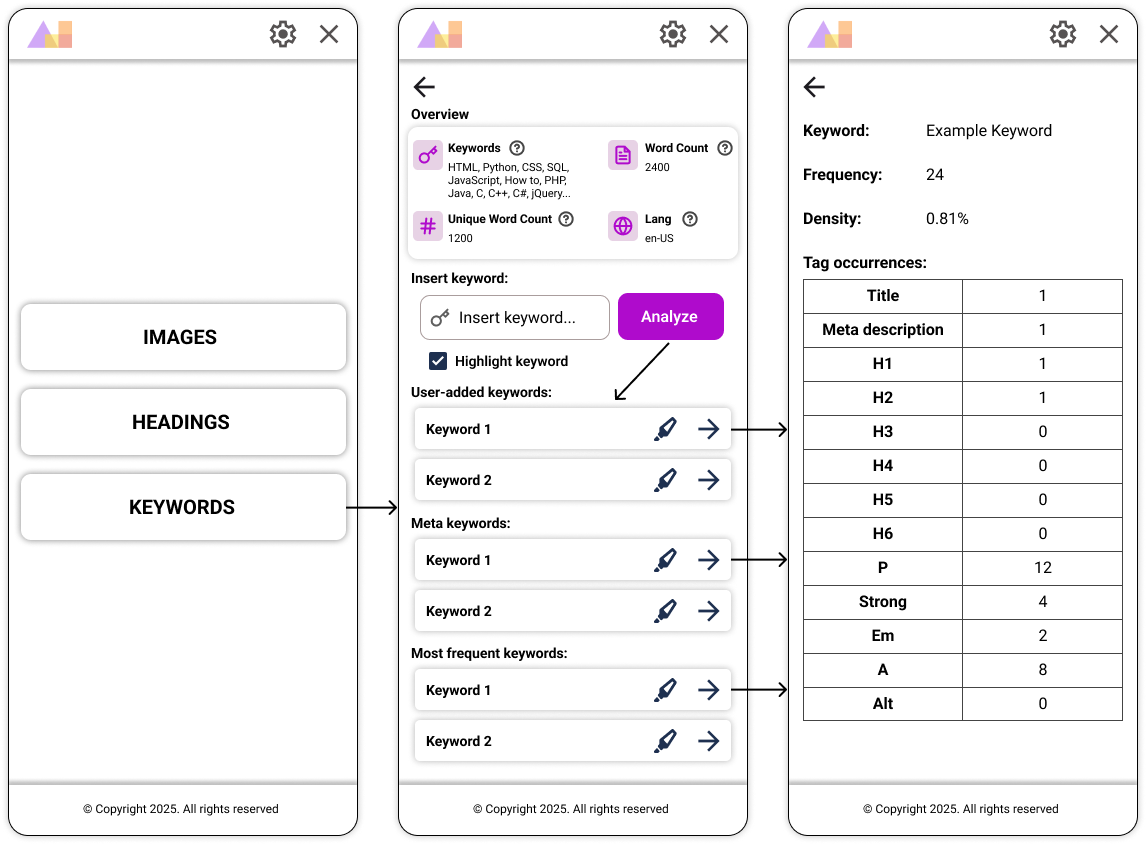
\includegraphics[width=\columnwidth]{progettazione/mockup.png} 
  \caption{Mockup dell'interfaccia grafica}
  \label{fig:mockup}
\end{figure}

\section{PoC}
\label{sec:poc}

Lo scopo principale del \gls{poc} è stato quello di tradurre in codice il \textit{mockup} dell’interfaccia grafica, al fine di verificare la correttezza e la coerenza delle scelte progettuali. Per raggiungere questo obiettivo, ho simulato il funzionamento dell’estensione in ambiente \gls{localhost}, sostituendo una pagina reale con una versione statica. Questa soluzione ha reso possibile lavorare in un ambiente di test controllato, all’interno del quale è stato possibile condurre uno studio di fattibilità e sperimentare le funzionalità di analisi e di evidenziazione visiva delle parole chiave. Al termine di questa fase, è stato organizzato un incontro con la Proponente per discutere i risultati ottenuti e le problematiche riscontrate, e identificare gli elementi da mantenere, modificare o integrare, in vista della successiva progettazione architetturale e dello sviluppo definitivo.

\section{Progettazione architetturale}
\label{sec:progettazione}

Il progetto adotta il \textit{pattern} architetturale MVC (Model-View-Controller) al fine di garantire una chiara separazione delle responsabilità tra i diversi componenti. Come illustrato in figura \ref{fig:pattern_mvc}, questo \gls{design-pattern} si articola in tre elementi principali, ciascuno con un ruolo preciso e ben definito:
\begin{itemize}
  \item \textbf{Model}: rappresenta il cuore dell’architettura. È responsabile della rappresentazione e della gestione interna dei dati, isolando le operazioni di manipolazione, archiviazione e accesso. Ha il compito di mantenere i dati organizzati, accurati e coerenti con le regole e la logica dell’applicazione;
  \item \textbf{View}: è il componente con cui l’utente interagisce direttamente. Visualizza i dati in un formato comprensibile e gestisce l’interazione tra l’utente e il sistema. Trattandosi di un componente “passivo”, la View non comunica direttamente con il Model, ma si affida al Controller per elaborare le richieste;
  \item \textbf{Controller}: funge da intermediario tra il Model e la View. Contiene la logica applicativa, elabora le richieste dell’utente e aggiorna il Model e la View di conseguenza. È responsabile della gestione del flusso dell’applicazione.
\end{itemize}

\vspace{5pt}
\noindent Il \textit{pattern} MVC promuove principi fondamentali della qualità del software, quali modularità, manutenibilità, scalabilità, robustezza e riusabilità. La chiara separazione delle responsabilità tra i componenti consente di limitare l’impatto delle modifiche, che possono essere applicate a un singolo modulo senza influire sugli altri. Inoltre, l’architettura MVC facilita l’esecuzione di test di unità e di integrazione, migliorando l’affidabilità del sistema.

\begin{figure}[H] 
  \centering 
  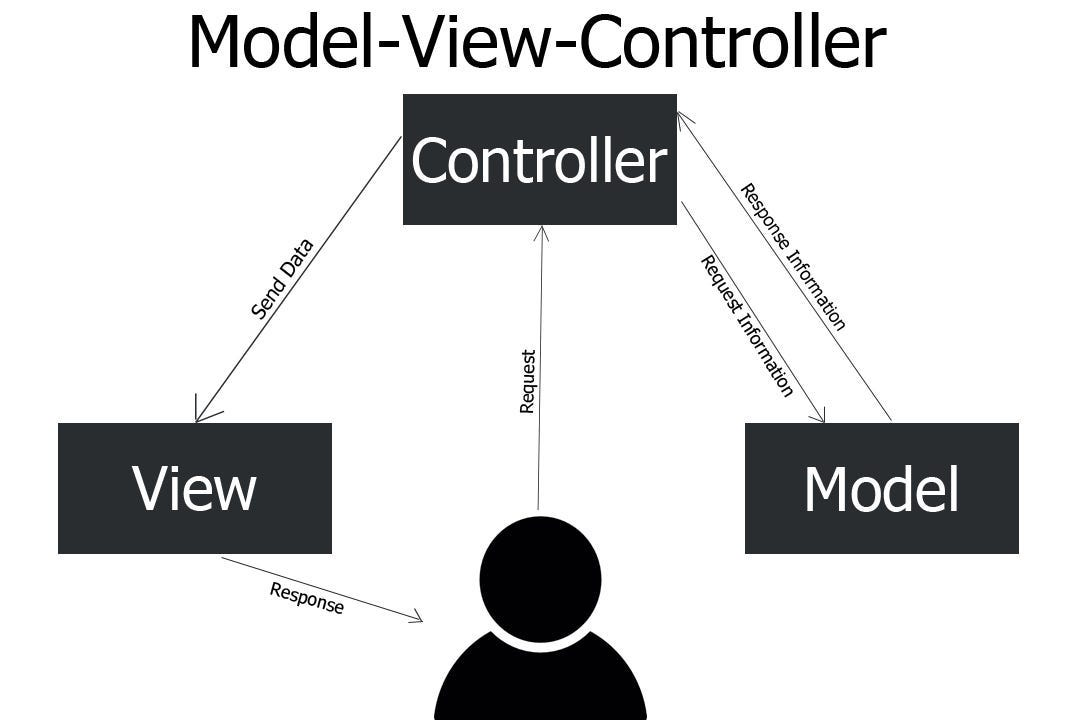
\includegraphics[width=0.6\textwidth]{progettazione/mvc.jpg} 
  \caption{Pattern MVC (Model-View-Controller)}
  \label{fig:pattern_mvc}
\end{figure}

\noindent 
\begin{minipage}{\textwidth}
  Di seguito è riportata la struttura dello strumento di analisi delle parole chiave:
  \vspace{10pt}
  \dirtree{%
    .1 .github.
    .2 workflows.
    .1 keyword.
    .2 controller.
    .2 model.
    .2 services.
    .3 strategy.
    .2 tests.
    .2 utils.
    .2 view.
    .1 static.
    .2 fonts.
    .2 img.
    .2 libs.
  }
\end{minipage}

\section{Design Pattern}
\label{sec:design-pattern}

Oltre al \textit{pattern} architetturale MVC (Model-View-Controller), ho adottato anche i \textit{pattern} Strategy e Dependency Injection.

\subsection{Strategy}

Strategy è un \gls{design-pattern} comportamentale che permette di incapsulare una famiglia di algoritmi e di selezionare dinamicamente quello più adatto. Poiché in \gls{javascript}, a differenza di linguaggi come \gls{java} o \gls{c-sharp}, non esistono interfacce in senso stretto, ho definito una classe che ne simula il comportamento all’interno del \textit{pattern} Strategy. Questa classe agisce come una struttura astratta: impedisce l'istanziazione diretta e impone l’implementazione dei metodi. Nell’ambito del progetto di stage, il \textit{pattern} Strategy è stato utilizzato per delegare una fase dell’analisi a due classi distinte, ognuna delle quali fornisce una diversa implementazione dello stesso processo. In questo modo è possibile selezionare dinamicamente l’algoritmo desiderato senza modificare il codice del modulo di analisi principale.

\vspace{10pt}
\noindent Entrambe le classi calcolano la frequenza complessiva di una parola chiave tramite la navigazione del \gls{dom} con \textit{TreeWalker}. Le differenze risiedono nel metodo utilizzato per determinare il numero di occorrenze all’interno di un insieme predefinito di tag \gls{html} ritenuti rilevanti per l’analisi. La classe \textit{StagedAnalysisStrategy} esegue un’analisi “per fasi” (staged), contando le occorrenze nei tag solo dopo aver completato il calcolo della frequenza complessiva. L’algoritmo accede direttamente ai tag e ne estrae il contenuto tramite la proprietà \textit{textContent}. Al contrario, la classe \textit{AllInOneAnalysisStrategy} effettua un’analisi compatta e unificata (all in one), registrando le occorrenze nei tag contestualmente al calcolo della frequenza. In questo caso, l’accesso ai tag avviene durante la navigazione del \gls{dom}, risalendo la gerarchia (con un approccio \textit{bottom-up}) ogni volta che vengono trovati \textit{match} all’interno di un nodo.

\subsection{Dependency Injection}

Dependency Injection è un \gls{design-pattern} che consente di fornire dall’esterno le dipendenze necessarie a un oggetto, invece di istanziarle al suo interno. Le due forme di injection più comuni sono:
\begin{itemize}
  \item \textbf{Constructor Injection}: la dipendenza viene iniettata mediante il costruttore della classe;
  \item \textbf{Setter Injection}: la dipendenza viene iniettata tramite un metodo setter.
\end{itemize}

\vspace{5pt}
\noindent Il \textit{pattern} Dependency Injection favorisce un basso accoppiamento tra i componenti, promuovendo principi fondamentali dell’ingegneria del software come la flessibilità, la manutenibilità, l’estensibilità, la modularità, la riusabilità e il testing. Nell’ambito del progetto di stage, l’adozione di questo \textit{pattern} si è rivelata particolarmente utile durante la scrittura dei test di unità e di integrazione, in quanto ha permesso di sostituire le dipendenze reali con oggetti fittizi (mock).

\section{Elenco delle classi}
\label{sec:elenco-classi}

\subsection{Model}

Di seguito sono elencate le classi presenti nella cartella \textit{Model}:

\begin{itemize}
  \item \textbf{Keyword}: rappresenta il modello relativo alle parole chiave. Memorizza il nome (cioè la keyword vera e propria), la frequenza, la densità, lo stato dell’analisi e il numero di occorrenze all’interno di un insieme predefinito di tag \gls{html} considerati rilevanti per l’analisi. Espone metodi \textit{getter} e \textit{setter} per l’interazione esterna, oltre a un metodo per ripristinare lo stato del modello e uno per calcolare la densità;
  \item \textbf{KeywordListInfo}: funge da DTO (Data Transfer Object) per la View, trasportando le informazioni associate a una lista di keyword, come la categoria (es. meta keywords e user-added keywords), il titolo, le parole chiave da visualizzare, il numero totale di pagine e la modalità di ordinamento;
  \item \textbf{OverviewInfo}: memorizza le informazioni relative all’anteprima dell’analisi \gls{seo}, come il contenuto del meta tag keywords, la lingua dichiarata nella pagina, il numero totale di parole e il conteggio delle parole uniche.
\end{itemize}

\subsection{View}

Di seguito sono elencate le classi presenti nella cartella \textit{View}:

\begin{itemize}
  \item \textbf{KeywordView}: visualizza la \textit{dashboard}, ovvero il pannello di controllo principale da cui è possibile anche aggiornare l’analisi a livello globale, e gestisce le operazioni di creazione, accesso e rimozione delle sottoview. La \textit{dashboard} è suddivisa nelle seguenti sezioni:
  \begin{itemize}
    \item \textbf{Overview}: mostra un’anteprima dell’analisi \gls{seo};
    \item \textbf{Settings}: visualizza le impostazioni dell’analisi \gls{seo}, che consentono di personalizzare i colori utilizzati per evidenziare le parole chiave;
    \item \textbf{Insert Keyword}: mostra un campo di \textit{input} affiancato da un pulsante per avviare l’analisi. Include anche una \textit{checkbox}, posizionata sotto il campo di \textit{input}, che permette di attivare l’evidenziazione della parola chiave digitata;
    \item \textbf{Keyword List}: visualizza un elenco di parole chiave organizzate per categoria (es. meta keywords e user-added keywords).
  \end{itemize}
  \item \textbf{KeywordListView}: visualizza una lista di keyword suddivisa in tre sezioni virtuali:
  \begin{itemize}
    \item \textbf{Header}: mostra il titolo della lista, un campo di \textit{input} per il filtraggio delle parole chiave, due pulsanti per l’ordinamento e un pulsante per la rimozione dei filtri;
    \item \textbf{Body}: visualizza l’elenco delle parole chiave, ciascuna accompagnata da un’indicazione della frequenza e un gruppo di pulsanti per l’eliminazione, l’evidenziazione e l’accesso ai risultati dell’analisi;
    \item \textbf{Footer}: mostra l’elenco delle pagine per navigare all’interno della lista.
  \end{itemize}
  \item \textbf{AnalysisResultView}: visualizza i risultati dell’analisi di una singola parola chiave, utilizzando un formato tabellare per riportare il numero di occorrenze nei singoli tag \gls{html}. Include anche un pulsante (highlighter) che consente di evidenziare direttamente una parola chiave e che rimane sincronizzato tra tutte le View.
\end{itemize}

\subsection{Controller}

Di seguito sono elencate le classi presenti nella cartella \textit{Controller}:

\begin{itemize}
  \item \textbf{KeywordController}: si occupa dell’inizializzazione e dell’aggiornamento dell’interfaccia, dell’associazione (binding) degli eventi e della gestione delle parole chiave, includendo funzionalità come inserimento, analisi, evidenziazione, eliminazione, navigazione, ordinamento e filtraggio.
\end{itemize}

\subsection{Services}

Di seguito sono elencate le classi presenti nella cartella \textit{Services}:

\begin{itemize}
  \item \textbf{TreeWalkerManager}: gestisce la creazione dell’oggetto \textit{TreeWalker}, definendo quali nodi includere o escludere nella navigazione del \gls{dom}. Fornisce inoltre un metodo per tornare alla radice e uno per accedere al nodo successivo;
  \item \textbf{TextProcessor}: fornisce funzioni di utilità condivise dai moduli di analisi ed evidenziazione. In particolare, espone i seguenti metodi:
  \begin{itemize}
    \item \textbf{getWordsPattern}: restituisce un'espressione regolare per estrarre le parole dal testo;
    \item \textbf{getCompoundSplitPattern}: restituisce un’espressione regolare per suddividere il testo in blocchi (proposizioni);
    \item \textbf{getKeywordPattern}: restituisce un’espressione regolare per identificare una parola chiave nel testo;
    \item \textbf{getParentName}: restituisce il nome dell’elemento genitore più vicino (risalendo la gerarchia del \gls{dom} con un approccio \textit{bottom-up}), tra quelli considerati rilevanti per l’analisi;
    \item \textbf{getTextNodes}: restituisce i nodi di testo;
    \item \textbf{getTextNodeGroups}: restituisce i nodi di testo suddivisi in gruppi. Ciascun gruppo contiene nodi \textit{inline} validi (come strong ed em) che condividono lo stesso elemento genitore.
  \end{itemize}
  \item \textbf{TagAccessor}: centralizza l’accesso ai tag \gls{html} e fornisce un metodo per estrarne il contenuto testuale;
  \item \textbf{WordCounter}: si occupa di calcolare il numero di parole presenti nella pagina e di identificare quelle più frequenti. Quest’ultima operazione è gestita da due metodi distinti, \textit{findOneWordKeywords} e \textit{findCompoundKeywords}, che estraggono rispettivamente le espressioni più ricorrenti composte da una sola parola e da due o più termini (n-grammi), escludendo le \gls{stopword} in base alla lingua dichiarata nella pagina.
  \item \textbf{KeywordHighlighter}: implementa la funzionalità di evidenziazione delle parole chiave, esponendo tre metodi principali:
  \begin{itemize}
    \item \textbf{highlightKeyword}: evidenzia tutte le occorrenze di una parola chiave adottando due approcci differenti, a seconda che si tratti di una keyword semplice o di una keyphrase. Entrambi gli approcci si basano sulla stessa funzione per applicare l’evidenziazione, ma differiscono nella modalità di ricerca. Per le keyword semplici la ricerca avviene nei singoli nodi di testo, mentre per le keyphrase viene eseguita su un testo virtuale che include uno o più nodi mappati correttamente;
    \item \textbf{removeHighlight}: rimuove l’evidenziazione eseguendo una normalizzazione del \gls{dom}, al fine di ripristinare il contenuto originale;
    \item \textbf{updateTagColors}: aggiorna i colori utilizzati per l’evidenziazione delle parole chiave e inietta nuovamente lo stile nella pagina.
  \end{itemize}
  \item \textbf{KeywordAnalyzer}: implementa la funzionalità di analisi delle parole chiave, delegando al \textit{pattern} Strategy una fase del processo, che riguarda il calcolo della frequenza tramite la navigazione del \gls{dom} con \textit{TreeWalker} e la registrazione del numero di occorrenze in specifici tag \gls{html}. Questa classe espone quattro metodi principali:
  \begin{itemize}
    \item \textbf{analyzeKeyword}: esegue l’analisi di una singola parola chiave;
    \item \textbf{analyzeKeywords}: esegue l’analisi di un gruppo (batch) di parole chiave, gestendo opportunamente la cache per ottimizzare l’esecuzione;
    \item \textbf{countOccurrencesInTag}: conta il numero di occorrenze di una parola chiave in un determinato tag;
    \item \textbf{fullRefresh}: ripristina la cache di tutti i moduli utilizzati per l’analisi.
  \end{itemize}
\end{itemize}

\subsubsection{Strategy}

Di seguito sono elencate le classi presenti nella cartella \textit{Strategy}:

\begin{itemize}
  \item \textbf{KeywordAnalysisStrategy}: simula un’interfaccia all’interno del \textit{pattern} Strategy, definendo il contratto che le classi concrete devono implementare;
  \item \textbf{StagedAnalysisStrategy}: calcola la frequenza di una parola chiave tramite la navigazione del \gls{dom}, analizzando singoli nodi di testo o gruppi di nodi a seconda della tipologia di keyword (keyword semplice o keyphrase). I due metodi, \textit{analyzeSimpleKeyword} e \textit{analyzeCompoundKeyword}, sono richiamati dal modulo di analisi principale. Per contare il numero di occorrenze all’interno di un insieme predefinito di tag \gls{html}, entrambi i metodi analizzano direttamente i tag interessati, separatamente rispetto al calcolo della frequenza;
  \item \textbf{AllInOneAnalysisStrategy}: calcola la frequenza in modo analogo alla classe precedente. La differenza principale riguarda la modalità con cui vengono contate le occorrenze all’interno di specifici tag \gls{html}. Rispetto alla classe precedente, il conteggio avviene contestualmente al calcolo della frequenza, risalendo la gerarchia del \gls{dom} con un approccio \textit{bottom-up}. Per le keyword semplici, l’analisi viene eseguita su singoli nodi di testo; in caso di \textit{match}, è sufficiente risalire la gerarchia alla ricerca dei tag interessati e registrare le occorrenze. Per le keyphrase, invece, l’analisi si svolge su un gruppo di nodi; la registrazione delle occorrenze richiede non solo di risalire la gerarchia per individuare i tag interessati, ma anche di filtrarli per mantenere quelli comuni a tutti i nodi \textit{matchati}.
\end{itemize}

\subsection{Utils}

Di seguito sono elencate le classi presenti nella cartella \textit{Utils}:

\begin{itemize}
  \item \textbf{Utils}: fornisce due funzioni di utilità, \textit{escapeRegExp} ed \textit{escapeHTML}, che consentono rispettivamente di eseguire l’escape di un’espressione regolare e di convertire alcuni caratteri predefiniti in entità \gls{html}. 
\end{itemize}

\subsection{Tracciamento dei requisiti - Implementazione}

La tabella \ref{tab:requisiti-implementazione} riporta l’associazione tra i requisiti funzionali e le classi che ne realizzano l’implementazione.

\renewcommand{\arraystretch}{1.5}
\begin{tabularx}{\textwidth}{l >{\raggedright\arraybackslash}X l}
  \caption{Tabella dei requisiti - Implementazione}
  \label{tab:requisiti-implementazione} \\
  \hline\hline
  \textbf{Requisito} & \textbf{Classi} & \textbf{\% di copertura}\\
  \endfirsthead

  \caption[]{Tabella dei requisiti - Implementazione (continua)} \\
  \hline\hline
  \textbf{Requisito} & \textbf{Classi} & \textbf{\% di copertura} \\
  \endhead

  \multicolumn{3}{r}{{Continua nella prossima pagina}} \\
  \endfoot

  \hline
  \endlastfoot

  \hline
  RF.O.1 & \texttt{Interface} & 100\% \\
  \hline 
  RF.O.2 & \texttt{KeywordController}, \texttt{WordCounter}, \texttt{OverviewInfo}, \texttt{KeywordView} & 100\% \\
  \hline 
  RF.O.3 & \texttt{KeywordController}, \texttt{OverviewInfo}, \texttt{KeywordView} & 100\% \\
  \hline 
  RF.O.4 & \texttt{KeywordController}, \texttt{WordCounter}, \texttt{OverviewInfo}, \texttt{KeywordView} & 100\% \\
  \hline 
  RF.D.5 & \texttt{KeywordController}, \texttt{WordCounter}, \texttt{OverviewInfo}, \texttt{KeywordView} & 100\% \\
  \hline 
  RF.O.6 & \texttt{KeywordController}, \texttt{OverviewInfo}, \texttt{KeywordView} & 100\% \\
  \hline 
  RF.O.7 & \texttt{KeywordController}, \texttt{KeywordView}, \texttt{KeywordListView} & 100\% \\
  \hline 
  RF.O.8 & \texttt{KeywordController}, \texttt{KeywordAnalyzer}, \texttt{StagedAnalysisStrategy}, \texttt{AllInOneAnalysisStrategy}, \texttt{Keyword}, \texttt{KeywordView}, \texttt{KeywordListView} & 100\% \\
  \hline 
  RF.O.9 & \texttt{KeywordController}, \texttt{Keyword}, \texttt{KeywordListInfo}, \texttt{KeywordView}, \texttt{KeywordListView} & 100\% \\
  \hline 
  RF.O.10 & \texttt{KeywordController}, \texttt{Keyword}, \texttt{KeywordListInfo}, \texttt{KeywordView}, \texttt{KeywordListView} & 100\% \\
  \hline 
  RF.O.11 & \texttt{KeywordController}, \texttt{Keyword}, \texttt{KeywordListInfo}, \texttt{KeywordView}, \texttt{KeywordListView} & 100\% \\
  \hline 
  RF.OP.12 & \texttt{KeywordController}, \texttt{WordCounter}, \texttt{Keyword}, \texttt{KeywordListInfo}, \texttt{KeywordView}, \texttt{KeywordListView} & 100\% \\
  \hline 
  RF.OP.13 & \texttt{KeywordController}, \texttt{WordCounter}, \texttt{Keyword}, \texttt{KeywordListInfo}, \texttt{KeywordView}, \texttt{KeywordListView} & 100\% \\
  \hline 
  RF.OP.14 & \texttt{KeywordController}, \texttt{WordCounter}, \texttt{Keyword}, \texttt{KeywordListInfo}, \texttt{KeywordView}, \texttt{KeywordListView} & 100\% \\
  \hline 
  RF.O.15 & \texttt{KeywordController}, \texttt{Keyword}, \texttt{KeywordListInfo}, \texttt{KeywordView}, \texttt{KeywordListView} & 100\% \\
  \hline 
  RF.O.16 & \texttt{KeywordController}, \texttt{KeywordHighlighter}, \texttt{Keyword}, \texttt{KeywordView} & 100\% \\
  \hline 
  RF.O.17 & \texttt{KeywordController}, \texttt{Keyword}, \texttt{AnalysisResultView} & 100\% \\
  \hline 
  RF.D.18 & \texttt{KeywordController}, \texttt{Keyword}, \texttt{KeywordView}, \texttt{KeywordListView} & 100\% \\
  \hline 
  RF.O.19 & \texttt{KeywordController}, \texttt{Keyword}, \texttt{KeywordListInfo}, \texttt{KeywordView}, \texttt{KeywordListView}, \texttt{AnalysisResultView} & 100\% \\
  \hline 
  RF.O.20 & \texttt{KeywordController}, \texttt{Keyword}, \texttt{KeywordListInfo}, \texttt{KeywordView}, \texttt{KeywordListView}, \texttt{AnalysisResultView} & 100\% \\
  \hline 
  RF.O.21 & \texttt{KeywordController}, \texttt{Keyword}, \texttt{KeywordView}, \texttt{AnalysisResultView} & 100\% \\
  \hline 
  RF.O.22 & \texttt{KeywordController}, \texttt{Keyword}, \texttt{KeywordView}, \texttt{AnalysisResultView} & 100\% \\
  \hline 
  RF.O.23 & \texttt{KeywordController}, \texttt{Keyword}, \texttt{KeywordView}, \texttt{AnalysisResultView} & 100\% \\
  \hline 
  RF.O.24 & \texttt{KeywordController}, \texttt{Keyword}, \texttt{KeywordView}, \texttt{AnalysisResultView} & 100\% \\
  \hline 
  RF.O.25 & \texttt{KeywordController}, \texttt{Keyword}, \texttt{KeywordView}, \texttt{AnalysisResultView} & 100\% \\
  \hline 
  RF.D.26 & \texttt{KeywordController}, \texttt{Keyword}, \texttt{KeywordView}, \texttt{KeywordListView} & 100\% \\
  \hline 
  RF.D.27 & \texttt{KeywordController}, \texttt{Keyword}, \texttt{KeywordView}, \texttt{KeywordListView} & 100\% \\
  \hline 
  RF.D.28 & \texttt{KeywordController}, \texttt{Keyword}, \texttt{KeywordView}, \texttt{KeywordListView} & 100\% \\
  \hline 
  RF.O.29 & \texttt{KeywordController}, \texttt{Keyword}, \texttt{KeywordView}, \texttt{KeywordListView} & 100\% \\
  \hline 
  RF.OP.30 & \texttt{KeywordController}, \texttt{WordCounter}, \texttt{KeywordAnalyzer}, \texttt{StagedAnalysisStrategy}, \texttt{AllInOneAnalysisStrategy}, \texttt{Keyword}, \texttt{OverviewInfo}, \texttt{KeywordView}, \texttt{KeywordListView} & 100\% \\
  \hline 
  RF.O.31 & \texttt{KeywordController}, \texttt{OverviewInfo}, \texttt{KeywordView} & 100\% \\
  \hline 
  RF.O.32 & \texttt{KeywordController}, \texttt{OverviewInfo}, \texttt{KeywordView} & 100\% \\
  \hline 
  RF.O.33 & \texttt{KeywordController}, \texttt{Keyword}, \texttt{KeywordListInfo}, \texttt{KeywordView}, \texttt{KeywordListView}, \texttt{AnalysisResultView} & 100\% \\
  \hline 
  RF.O.34 & \texttt{KeywordController}, \texttt{Keyword}, \texttt{KeywordView}, \texttt{AnalysisResultView} & 100\% \\
  \hline 
  RF.OP.35 & \texttt{KeywordController}, \texttt{KeywordHighlighter}, \texttt{KeywordView} & 100\% \\
  \hline 
  RF.OP.36 & \texttt{KeywordController}, \texttt{KeywordHighlighter}, \texttt{KeywordView} & 100\% \\
  \hline 
  RF.OP.37 & \texttt{KeywordController}, \texttt{KeywordHighlighter}, \texttt{KeywordView} & 100\% \\
  \hline 
  RF.OP.38 & \texttt{KeywordController}, \texttt{KeywordHighlighter}, \texttt{KeywordView} & 100\% \\
  \hline 
  RF.O.39 & \texttt{KeywordController}, \texttt{KeywordAnalyzer}, \texttt{StagedAnalysisStrategy}, \texttt{AllInOneAnalysisStrategy}, \texttt{Keyword} & 100\% \\
  \hline 
  RF.OP.40 & \texttt{KeywordController}, \texttt{KeywordAnalyzer}, \texttt{StagedAnalysisStrategy}, \texttt{AllInOneAnalysisStrategy}, \texttt{Keyword} & 100\% \\
  \hline 
  RF.O.41 & \texttt{KeywordHighlighter} & 100\% \\
  \hline 
  RF.OP.42 & \texttt{WordCounter} & 100\% \\
  \hline 
  RF.D.43 & \texttt{WordCounter}, \texttt{KeywordAnalyzer}, \texttt{StagedAnalysisStrategy}, \texttt{AllInOneAnalysisStrategy}, \texttt{KeywordHighlighter} & 100\% \\
\end{tabularx}
        \chapter{Funzionalità sviluppate}
\label{cap:funzionalità-sviluppate}

\section{Evidenziazione delle parole chiave}
\label{sec:highlight-keyword}

\par La funzionalità “Highlight Keywords” consente di evidenziare tutte le occorrenze di una parola chiave all’interno della pagina web in cui l’estensione è attiva. Ogni occorrenza viene formattata con colori di sfondo, testo e bordo differenti, in base al tag \gls{html} che la contiene; tali colori sono personalizzabili tramite le impostazioni dell’estensione. Oltre alla personalizzazione cromatica delle occorrenze, ciascuna di esse è accompagnata da un’etichetta, posizionata in alto a sinistra, che riporta il nome del tag genitore. Nell’interfaccia grafica, a ogni keyword è associato un pulsante (highlighter) che permette di attivare o disattivare l’evidenziazione a livello globale. Questa funzionalità è accessibile sia dalla pagina principale sia da quella dedicata a una singola keyword, e lo stato del pulsante rimane sincronizzato tra le due. Le parole chiave inserite manualmente dall'utente possono essere evidenziate anche prima dell’avvio dell’analisi vera e propria, tramite il pulsante dedicato, mantenendo le funzionalità di analisi ed evidenziazione separate e indipendenti.

\subsection{Problematiche riscontrate}

\par La prima difficoltà è stata individuare un metodo efficiente per navigare il \gls{dom}, escludendo al contempo gli elementi non rilevanti dal punto di vista \gls{seo}. Tra le opzioni considerate, l’oggetto \textit{TreeWalker} si è dimostrato il più adatto, in quanto permette di gestire in modo centralizzato la logica di filtraggio dei nodi, determinando in modo preciso quali accettare o scartare. La sfida successiva ha riguardato la definizione del criterio di ricerca delle parole chiave. A differenza di strumenti come \textit{MozBar}, ho scelto di non evidenziare le occorrenze che compaiono come sottostringhe all’interno di parole più lunghe (ad esempio “Java” all’interno di “JavaScript”). In fase di ricerca, parole separate da un punto, un trattino (alto o basso) o un apostrofo vengono considerate un’unica parola. Tutti gli altri caratteri sono trattati come separatori, in modo analogo a quanto avviene nell’estensione \textit{SEOquake}.

\vspace{10pt}
\par\noindent Una volta individuate le occorrenze di una parola chiave, l’evidenziazione è stata applicata utilizzando un oggetto \textit{DocumentFragment}, che permette di costruire in modo sicuro una struttura temporanea da inserire nel DOM principale. Per rimuovere l’evidenziazione e ripristinare correttamente il contenuto originale, è stata eseguita un’operazione di normalizzazione del DOM, tramite la quale i nodi di testo adiacenti vengono unificati e quelli vuoti rimossi.

\vspace{10pt}
\par\noindent Un altro ostacolo, particolarmente critico per l’affidabilità e le prestazioni del sistema, è emerso nel trattamento delle parole chiave composte da più termini separati da spazi (note anche come \textit{keyphrase}). L’approccio iniziale prevedeva l’esecuzione della ricerca sui singoli nodi di testo; di conseguenza, una keyword come “JavaScript Tutorial” non veniva riconosciuta se i due termini erano distribuiti su tag distinti (ad esempio, un h1 e uno span annidato). Questo limite è stato rilevato nel corso di test manuali condotti su un blog di intrattenimento e informazione, che adotta una convenzione particolare: evidenziare in grassetto solo il cognome all’interno dei nomi propri. Ciò comportava la frammentazione di molte \textit{keyphrase}, che non venivano identificate correttamente dal sistema. Per rendere la ricerca delle \textit{keyphrase} più granulare e accurata, ho sviluppato due algoritmi: uno ricorsivo e uno iterativo. Il primo suddivide la \textit{keyphrase} in blocchi e cerca ciascun blocco all’interno di nodi di testo adiacenti. Il secondo, invece, costruisce un testo virtuale concatenando il contenuto di nodi adiacenti, simulando il comportamento delle proprietà \textit{innerText} o \textit{textContent}. In entrambi gli approcci, i nodi adiacenti devono appartenere allo stesso contesto, ovvero condividere lo stesso elemento genitore ed essere elementi \textit{inline}. Tra le due soluzioni, è stato preferito il secondo algoritmo, in quanto più flessibile e maggiormente coerente con il comportamento reale del browser.

\vspace{10pt}
\par\noindent Nel secondo algoritmo, ogni volta che si concatena il contenuto di un nodo al testo virtuale, è necessario effettuare una mappatura degli indici di inizio e fine, in modo da poter risalire al nodo originale nel momento in cui viene trovata una corrispondenza. Questa operazione può risultare complessa, soprattutto in presenza di \gls{dom} profondi o fortemente nidificati. Per questo motivo, l’algoritmo “a nodi multipli” non ha sostituito quello originale, che esegue la ricerca sui singoli nodi di testo, ma coesiste con esso all’interno del sistema. I due algoritmi vengono richiamati dinamicamente in base alla tipologia di parola chiave: per le keyword semplici viene utilizzato l’algoritmo “a nodo singolo”, mentre per le keyphrase viene impiegato l’algoritmo “a nodi multipli”. È stato valutato anche il caso limite in cui una keyword semplice risulti spezzata su più tag. Tuttavia, trattandosi di una situazione molto rara, si è deciso di non complicare ulteriormente il flusso di ricerca per gestirla.

\section{Analisi delle parole chiave}
\label{sec:analyze-keyword}

\par La funzionalità “Analyze Keywords” è stata progettata per operare principalmente su pagine web in lingua inglese e italiana. Questa funzionalità fornisce una panoramica generale dell'analisi \gls{on-page-seo}, che include i seguenti elementi:
\begin{itemize}
  \item Contenuto del meta tag keywords;
  \item Lingua dichiarata nella pagina;
  \item Conteggio totale delle parole;
  \item Conteggio delle parole uniche.
\end{itemize}

\vspace{10pt}
\par\noindent Queste informazioni costituiscono la base per l'analisi delle parole chiave, che prende in considerazione diversi parametri, come la frequenza, la densità e il numero di occorrenze all’interno di un insieme predefinito di tag semantici. L'analisi viene eseguita su una copia statica del \gls{dom}, al fine di garantire coerenza tra tutte le parole chiave, e può essere aggiornata manualmente tramite un pulsante dedicato. La ricerca delle parole chiave segue gli stessi criteri illustrati nella \hyperref[sec:highlight-keyword]{sezione \textsection\ref*{sec:highlight-keyword}}.

\vspace{10pt}
\par\noindent I tag semantici considerati più rilevanti dal punto di vista SEO sono:
\begin{itemize}
  \item Il tag title;
  \item Il meta tag description;
  \item I tag di intestazione (H1-H6);
  \item I paragrafi (<p>);
  \item I link (<a>);
  \item Il testo in grassetto (<strong>);
  \item Il test in corsivo (<em>);
  \item Le voci degli elenchi (<li>);
  \item Il testo alternativo delle immagini (Alt).
\end{itemize}

\vspace{10pt}
\par\noindent Per il calcolo delle occorrenze di una parola chiave all’interno di questi tag, sono stati adottati due approcci:
\begin{itemize}
  \item Accedere direttamente ai tag e utilizzare la proprietà textContent per estrarne il contenuto da analizzare;
  \item Risalire ai tag semantici durante la navigazione del DOM con \textit{TreeWalker}, registrando le occorrenze contestualmente al calcolo della frequenza complessiva.
\end{itemize}

\vspace{10pt}
\par\noindent Poiché entrambi gli approcci sono stati considerati ugualmente validi, ho adottato il design pattern comportamentale \textit{Strategy}, in modo da poter selezionare dinamicamente l’algoritmo senza alterare il codice del modulo di analisi.

\subsection{Problematiche riscontrate}

\par Una delle difficoltà incontrate ha riguardato il calcolo di un punteggio da associare a ciascuna parola chiave. Le due opzioni considerate erano l’assegnazione di un punteggio di qualità o, in alternativa, di un punteggio basato sulla rilevanza strutturale. Tuttavia, in entrambi i casi è emerso che i criteri effettivamente utilizzati dai motori di ricerca sono molto più articolati e difficili da replicare in modo attendibile. Per questo motivo, ho concordato con la Proponente di non introdurre alcun sistema di punteggio.

\vspace{10pt}
\par\noindent Un’altra problematica è stata riscontrata in seguito alla modifica della modalità di analisi, con il passaggio dal \gls{dom} live a una copia statica. Durante l’operazione di clonazione, infatti, gli stili applicati agli elementi non vengono mantenuti, rendendo meno preciso il controllo sui tag \textit{inline} rispetto a quanto avviene nella funzionalità di evidenziazione, che opera direttamente sul DOM live. Tuttavia, in fase di analisi, è possibile fare affidamento sulla natura semantica dei tag \gls{html}. Pertanto, un controllo basato sul nome del tag risulta sufficiente nella maggior parte dei casi, garantendo un buon livello di affidabilità anche senza una verifica esplicita dello stile.

\vspace{10pt}
\par\noindent Un aspetto che ha generato ambiguità è stata la discrepanza tra la frequenza complessiva e la somma delle occorrenze rilevate nei singoli tag. Tale divergenza era dovuta al fatto che alcune occorrenze di una parola chiave si trovavano all’interno di tag annidati. La soluzione concordata con la Proponente è stata l’inserimento di un messaggio esplicativo, al fine di chiarire il comportamento del sistema ed evitare fraintendimenti da parte dell’utente.

\section{Conteggio delle parole ed estrazione di quelle più frequenti}
\label{sec:count-word}

\par Il conteggio delle parole presenti nella pagina rappresenta un requisito fondamentale per il calcolo della densità di una keyword. L'estrazione delle parole dal testo avviene secondo un pattern che segue gli stessi criteri descritti nella \hyperref[sec:highlight-keyword]{sezione \textsection\ref*{sec:highlight-keyword}}. Tra i requisiti opzionali figura invece l'identificazione delle parole più frequenti, suddivisibili in categorie come “single-word”, “double-word” e così via. Questa funzionalità risulta particolarmente utile qualora il meta tag \textit{keywords} non sia presente, poiché consente di suggerire all’utente un elenco di termini che, in base alla frequenza, possono essere considerati potenziali parole chiave. Il sistema seleziona le 10 parole più ricorrenti per ciascuna categoria, presentandole in ordine decrescente.

\subsection{Problematiche riscontrate}

\par Le \gls{stopword} devono essere escluse dal processo di identificazione delle parole più frequenti, in quanto non hanno valore semantico e difficilmente corrispondono a parole chiave. A tal fine, ho utilizzato una libreria esterna per definire una serie di liste di stopword, selezionate dinamicamente in base alla lingua dichiarata nella pagina. Nel caso delle “single-word”, l’esclusione delle stopword è diretta e immediata. La gestione delle espressioni composte da due o più termini (n-grammi), invece, richiede maggiore attenzione. Nei testi in lingua italiana, ad esempio, è piuttosto comune l’uso di termini o espressioni in inglese (lingua di riferimento a livello internazionale). In questi contesti, espressioni come “The Batman” possono essere considerate valide, mentre sequenze prive di valore semantico come “of the” andrebbero escluse. Per trattare in modo adeguato queste situazioni, ho implementato un duplice controllo: escludere tutte le stopword relative alla lingua dichiarata nella pagina e tollerare la presenza di stopword inglesi solo se queste non superano il 50\% dei termini dell’espressione.

\section{Elenco delle parole chiave}
\label{sec:keyword-list}

\par L'interfaccia grafica è organizzata in quattro elenchi distinti: 
\begin{itemize}
  \item \textbf{Meta keywords}: parole chiave estratte dal meta tag keywords;
  \item \textbf{User-added keywords}: parole chiave inserite manualmente dall'utente;
  \item \textbf{Most frequent “single-word” keywords}: le 10 parole chiave più frequenti composte da una sola parola;
  \item \textbf{Most frequent “double-word” keywords}: le 10 parole chiave più frequenti composte da due parole.
\end{itemize}

\vspace{10pt}
\par\noindent Ogni elenco può essere ordinato per frequenza, filtrato per nome e ripristinato tramite appositi pulsanti. All’interno di ciascuna lista, il sistema carica 5 elementi alla volta, navigabili attraverso un sistema di paginazione. Per evitare di sovraccaricare l’interfaccia, non vengono mostrati tutti i pulsanti di navigazione delle pagine, ma solo un sottoinsieme calcolato dinamicamente secondo le seguenti regole:
\begin{itemize}
  \item Il pulsante per accedere alla prima pagina è sempre visibile;
  \item Il pulsante per accedere all’ultima pagina è sempre visibile;
  \item Sono visibili i due pulsanti precedenti a quello attualmente attivo;
  \item Sono visibili i due pulsanti successivi a quello attualmente attivo;
  \item I pulsanti nascosti sono sostituiti dalla stringa “...”.
\end{itemize}

\vspace{10pt}
\par\noindent A ciascuna keyword è associata un’indicazione della frequenza e un gruppo di pulsanti che consentono di eseguire operazioni come l’eliminazione, l’evidenziazione visiva o la visualizzazione dei risultati dell’analisi.

\subsection{Problematiche riscontrate}

\par L’elenco delle parole chiave più frequenti viene visualizzato, per impostazione predefinita, in ordine decrescente. Di conseguenza, il relativo pulsante di ordinamento deve risultare attivo sin dall’inizio. Una volta rimossi eventuali filtri, è necessario ripristinare il comportamento predefinito, ovvero riattivare il pulsante di ordinamento in modalità “desc”. Questa condizione è rimasta inosservata fino all’esecuzione dei test manuali, rendendo necessario un leggero refactoring per evitare potenziali situazioni di disorientamento per l’utente.

\section{Accessibilità}

\par Dal momento che la funzionalità di analisi delle parole chiave è integrata in un’estensione preesistente orientata all’accessibilità, anche questa componente è stata progettata in conformità alle linee guida \gls{wcag}. A tal fine, sono stati condotti test di accessibilità con i seguenti obiettivi:
\begin{itemize}
  \item Verificare il rispetto del \textbf{rapporto minimo di contrasto} tra testo e sfondo, pari a 4.5:1 per il testo di dimensioni “normali” e 3:1 per il testo di grandi dimensioni. Questo controllo è stato applicato sia agli elementi interni all’estensione, sia a quelli utilizzati per evidenziare le parole chiave;
  \item Controllare che le \textbf{immagini non decorative} siano dotate di un testo alternativo;
  \item Accertarsi che le \textbf{icone non decorative} siano accompagnate da un’etichetta accessibile;
  \item Verificare l’accessibilità dei \textbf{tooltip}, assicurandosi che vengano attivati e disattivati correttamente quando si interagisce con l’elemento trigger, sia tramite navigazione da tastiera sia tramite l’uso del mouse. Inoltre, i tooltip devono rimanere visibili al passaggio del mouse su di essi e devono poter essere chiusi premendo il tasto Esc;
  \item Controllare che tutti gli \textbf{elementi interattivi} (come pulsanti o link) dispongano di un’etichetta testuale descrittiva;
  \item Assicurare la \textbf{navigazione tramite tastiera}, con un ordine di tabulazione logico e una chiara indicazione visiva dell’elemento attualmente attivo.
\end{itemize}

        \chapter{Verifica e validazione}
\label{cap:verifica-validazione}

In questa sezione sono riportati i test effettuati durante lo svolgimento del progetto. La fase di testing è stata suddivisa in due sottofasi: verifica e validazione (V\&V). La verifica consiste nell’accertare che il software sia conforme alle specifiche, e può essere condotta senza eseguire il codice. Le attività di analisi statica includono la revisione e l’ispezione dei processi, dei \gls{requisiti}, del design e del codice sorgente. Quest’ultima può avvenire tramite una lettura approfondita del codice o mediante una revisione sistematica e mirata. La validazione, invece, riguarda l’analisi dinamica del software, finalizzata ad accertare il soddisfacimento dei \gls{requisiti} e delle aspettative dal punto di vista dell’utente finale. Le attività di validazione comprendono sia test automatici che manuali.

\lstdefinelanguage{JavaScript}{
  keywords={break, case, catch, continue, debugger, default, delete, do, else, finally, for, function, if, in, instanceof, new, return, switch, this, throw, try, typeof, var, void, while, with, let, const},
  keywordstyle=\color{blue}\bfseries,
  ndkeywords={class, export, boolean, throw, implements, import, this},
  ndkeywordstyle=\color{darkgray}\bfseries,
  identifierstyle=\color{black},
  sensitive=false,
  comment=[l]{//},
  morecomment=[s]{/*}{*/},
  commentstyle=\color{gray}\ttfamily,
  stringstyle=\color{red}\ttfamily,
  morestring=[b]',
  morestring=[b]"
}

\section{Test automatici}

Il testing automatizzato è una tecnica che prevede la configurazione di un ambiente di test e la progettazione di una o più suite che vengono eseguite automaticamente, confrontando i risultati effettivi con quelli attesi. Ogni test dovrebbe essere veloce, indipendente, affidabile e riutilizzabile. I test automatici non sostituiscono i test manuali né eliminano la necessità di una revisione “umana”; tuttavia, forniscono una misura oggettiva della qualità del software e contribuiscono a ottimizzare il ciclo di sviluppo, individuando rapidamente errori che potrebbero sfuggire all’osservazione manuale, specialmente in contesti di \gls{continuous integration}.

\vspace{10pt}
\noindent La progettazione, scrittura e manutenzione dei test automatici hanno richiesto uno sforzo considerevole; tuttavia, data la ridotta finestra temporale dello stage, l’automatizzazione si è rivelata essenziale nel lungo periodo. Essa ha infatti fornito un riscontro continuo sulla qualità del software durante lo sviluppo, riducendo il carico di lavoro legato all’esecuzione dei test manuali. Inoltre, ha consentito di raggiungere una copertura del codice del 100\% (come attestato dal report di Codecov in figura \ref{fig:report_codecov}), un risultato difficilmente ottenibile con il solo testing manuale.

\begin{figure}[H]
  \centering 
  \fbox{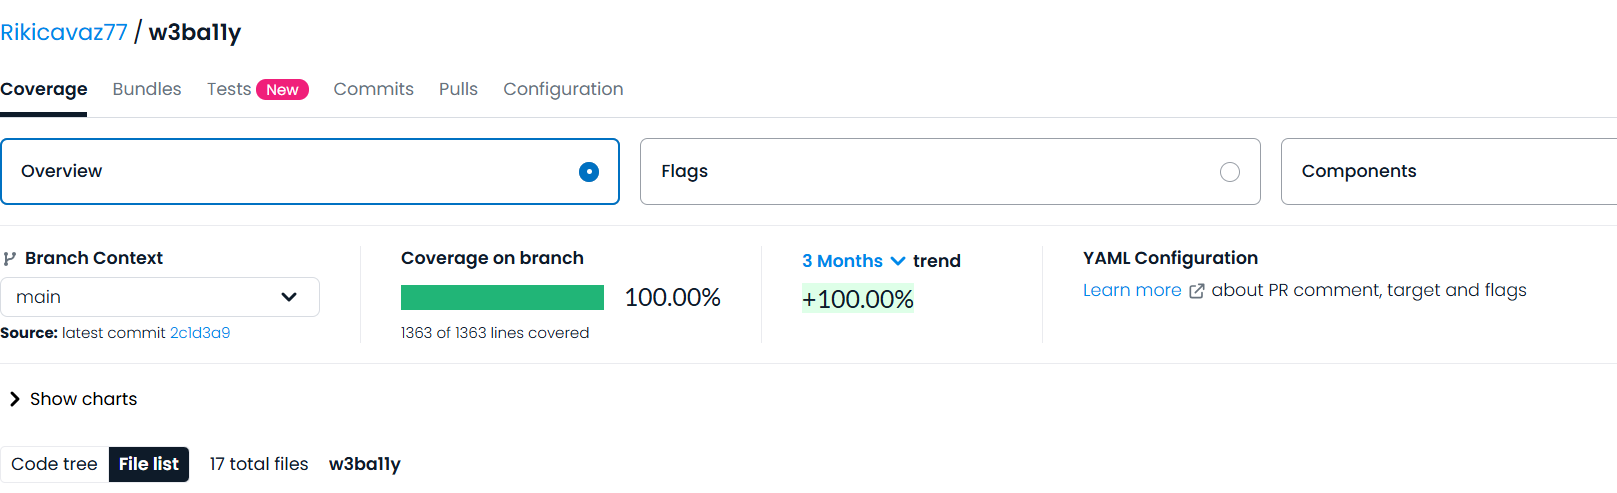
\includegraphics[width=0.9\columnwidth]{test/coverage.png}}
  \caption{Copertura del codice - report di Codecov}
  \label{fig:report_codecov}
\end{figure}

\noindent I test automatici vengono eseguiti a ogni apertura, aggiornamento o chiusura di una \gls{pull request}, garantendo che tutto il codice rilasciato superi i test e mantenga una copertura uniforme. Dal punto di vista architetturale e organizzativo, i test rispecchiano fedelmente la struttura del \textit{core} dell’estensione, risultando più leggibili e manutenibili. 

\vspace{10pt}
\begin{samepage}
  \dirtree{%
    .1 tests.
    .2 controller.
    .2 model.
    .2 services.
    .3 strategy.
    .2 utils.
    .2 view.
  }
\end{samepage}

\vspace{10pt}
\noindent Per mantenere l’isolamento tra l'estensione e l’ambiente di test, ciascun file testato deve terminare con la seguente porzione di codice:

\vspace{10pt}
\begin{samepage}
\begin{lstlisting}[language=JavaScript]
  /* istanbul ignore next */
  if (typeof module !== 'undefined' && typeof module.exports !== 'undefined') {
    module.exports = KeywordHighlighter;
  }
\end{lstlisting}
\end{samepage}

\vspace{10pt}
\noindent Questo approccio consente di importare i moduli all’interno dei file di test tramite la seguente istruzione:

\vspace{10pt}
\begin{samepage}
\begin{lstlisting}[language=JavaScript]
  const KeywordHighlighter = require('@keyword/services/keyword_highlighter');
\end{lstlisting}
\end{samepage}

\vspace{10pt}
\noindent La tabella \ref{tab:test-automatici} riporta i test di unità e di integrazione eseguiti.

\renewcommand{\arraystretch}{1.5}
\begin{longtable}{>{\raggedright\arraybackslash}p{0.65\textwidth} >{\raggedright\arraybackslash}p{0.25\textwidth}}
\caption{Tabella dei test automatici}
\label{tab:test-automatici} \\
\hline\hline
\textbf{Suite di test} & \textbf{\% di superamento dei test}\\
\endfirsthead
    
\caption[]{Tabella dei test automatici (continua)} \\
\hline\hline
\textbf{Suite di test} & \textbf{\% di superamento dei test} \\ 
\endhead
    
\multicolumn{2}{r}{{Continua nella prossima pagina}} \\ 
\endfoot
    
\hline
\endlastfoot

\hline
\textbf{Keyword} \textit{(keyword.test.js)}: verifica il corretto funzionamento del modello relativo alle parole chiave. & 100\% \\
\hline
\textbf{AnalysisResultView} \textit{(analysis\_result\_view.test.js)}: verifica il corretto funzionamento del componente responsabile della visualizzazione dei risultati relativi all’analisi di una parola chiave. & 100\% \\
\hline 
\textbf{KeywordListView} \textit{(keyword\_list\_view.test.js)}: verifica il corretto funzionamento del componente responsabile della visualizzazione delle liste di parole chiave per ciascuna tipologia. & 100\% \\
\hline 
\textbf{KeywordView} \textit{(view.test.js)}: verifica il corretto funzionamento della view principale, responsabile della gestione della \textit{dashboard} e delle sottoview. & 100\% \\
\hline 
\textbf{KeywordController} \textit{(controller.test.js)}: verifica il corretto funzionamento delle operazioni di gestione delle parole chiave (funzionalità non dipendenti dal \gls{dom} e non sufficientemente specifiche da giustificare una suite dedicata). & 100\% \\
\hline 
\textbf{KeywordController - DOM} \textit{(controller\_dom.test.js)}: verifica il corretto funzionamento delle operazioni del controller che richiedono l’interazione con il \gls{dom}. & 100\% \\
\hline 
\textbf{KeywordController - sorting} \textit{(controller\_sorting.test.js)}: verifica la funzionalità di ordinamento delle parole chiave. & 100\% \\
\hline
\textbf{KeywordController - filtering} \textit{(controller\_filtering.test.js)}: verifica la funzionalità di filtraggio delle parole chiave. & 100\% \\
\hline
\textbf{KeywordController - pagination} \textit{(controller\_pagination.test.js)}: verifica la logica di gestione della paginazione delle parole chiave. & 100\% \\
\hline
\textbf{KeywordController - highlight} \textit{(controller\_highlight.test.js)}: verifica la logica di gestione dell’evidenziazione delle parole chiave. & 100\% \\
\hline
\textbf{KeywordController - events} \textit{(controller\_events.test.js)}: verifica il corretto funzionamento dell’associazione (binding) degli eventi. & 100\% \\
\hline
\textbf{KeywordController - init} \textit{(controller\_init.test.js)}: verifica le funzionalità di inizializzazione e di aggiornamento del controller, nonché l’integrazione tra i componenti dell’architettura. & 100\% \\
\hline
\textbf{TreeWalkerManager} \textit{(tree\_walker\_manager.test.js)}: verifica la corretta gestione dell’oggetto \textit{TreeWalker}. & 100\% \\
\hline
\textbf{TextProcessor} \textit{(text\_processor.test.js)}: verifica il corretto comportamento delle funzioni di utilità legate all’analisi e all’elaborazione testuale. & 100\% \\
\hline
\textbf{TagAccessor} \textit{(tag\_accessor.test.js)}: verifica il corretto comportamento delle funzioni di utilità dedicate all’accesso e alla lettura del contenuto dei tag \gls{html}. & 100\% \\
\hline
\textbf{WordCounter} \textit{(word\_counter.test.js)}: verifica le funzionalità di conteggio delle parole e di estrazione di quelle più frequenti. & 100\% \\
\hline
\textbf{KeywordHighlighter} \textit{(keyword\_highlighter.test.js)}: verifica la funzionalità di evidenziazione delle parole chiave all’interno della pagina. & 100\% \\
\hline
\textbf{KeywordAnalyzer} \textit{(keyword\_analyzer.test.js)}: verifica la funzionalità di analisi delle parole chiave. & 100\% \\
\hline
\textbf{KeywordAnalysisStrategy} \textit{(keyword\_analysis\_strategy.test.js)}: verifica il corretto comportamento della struttura astratta, assicurandosi che l’istanziazione diretta sia impedita e che i metodi non implementati generino un errore. & 100\% \\
\hline
\textbf{StagedAnalysisStrategy} \textit{(staged\_analysis\_strategy.test.js)}: verifica il corretto funzionamento dell’implementazione concreta della \textit{strategy}, basata su un’analisi “per fasi” (staged). & 100\% \\
\hline
\textbf{AllInOneAnalysisStrategy} \textit{(all\_in\_one\_analysis\_strategy.test.js)}: verifica il corretto funzionamento dell’implementazione concreta della \textit{strategy}, basata su un’analisi compatta e unificata. & 100\% \\
\hline
\textbf{Utils} \textit{(utils.test.js)}: verifica il corretto comportamento delle funzioni di utilità. & 100\% \\
\end{longtable}

\section{Test manuali}

L’estensione è stata testata su un insieme di pagine web differenti per dimensione (in termini di profondità del \gls{dom}) e lingua (inglese o italiana), con l’obiettivo di verificarne il corretto funzionamento mediante osservazione manuale. La tabella \ref{tab:test-manuali} riporta i test manuali eseguiti.

\renewcommand{\arraystretch}{1.5}
\begin{tabularx}{\textwidth}{>{\raggedright\arraybackslash}X >{\raggedright\arraybackslash}X}
\caption{Tabella dei test manuali}
\label{tab:test-manuali} \\
\hline\hline
\textbf{Sito web} & \textbf{Esito dei test}\\
\endfirsthead
    
\caption[]{Tabella dei test manuali (continua)} \\
\hline\hline
\textbf{Sito web} & \textbf{Esito dei test} \\ 
\endhead
    
\multicolumn{2}{r}{{Continua nella prossima pagina}} \\ 
\endfoot
    
\hline
\endlastfoot

\hline
\textbf{W3Schools} - JavaScript Tutorial (\url{https://www.w3schools.com/js/}) & Tutti i test manuali sono stati superati con successo, inclusa l'analisi di parole chiave “spezzate” su più tag \gls{html} (es. “JavaScript Tutorial”). L’unica eccezione riscontrata nelle prime fasi di sviluppo riguardava il mancato rilevamento dei meta tag keywords e description. Il problema era dovuto al fatto che, contrariamente alle convenzioni più comuni, il valore dell’attributo \textit{name} iniziava con una lettera maiuscola. La soluzione adottata è stata l’aggiunta del flag di confronto “case-insensitive” nel selettore. \\
\hline
\textbf{W3Schools} - JavaScript Regular Expressions (\url{https://www.w3schools.com/js/js\_regexp.asp}) & Tutti i test manuali sono stati superati con successo. \\
\hline
\textbf{Corriere della Sera} - HomePage (\url{https://www.corriere.it/}) & Tutti i test manuali sono stati superati con successo, sebbene con prestazioni non sempre ottimali, a causa della complessità del sito in questione. \\
\hline
Siti web partecipanti al concorso \textbf{Accattivante Accessibile}, organizzato dall’Università degli Studi di Padova (\url{https://web.math.unipd.it/CAA/classifica.html}) & Tutti i test manuali sono stati superati con successo. Durante l’analisi del sito \textit{BookOverflow}, è emerso un caso particolare non gestito: una singola parola “spezzata” su più tag \gls{html} (es. “BookOverflow”). Questa situazione è stata valutata come un’eccezione poco significativa, non tale da giustificare una gestione più granulare, che avrebbe inciso negativamente sulle prestazioni. \\
\hline
\textbf{Nasce, Cresce, Ignora} - The Killer, la recensione (\url{https://nascecresceignora.it/the-killer-la-recensione-un-thriller-freddo-e-glaciale/}) & Tutti i test manuali sono stati superati con successo, inclusa l'analisi di parole chiave “spezzate” su più tag \gls{html} (es. “David Fincher”) e l’estrazione delle keyphrase più frequenti (es. “The Killer”). \\
\hline
\textbf{Nasce, Cresce, Ignora} - Pixar: I migliori film (\url{https://nascecresceignora.it/pixar-i-migliori-film-secondo-letterboxd/}) & Tutti i test manuali sono stati superati con successo. \\
\hline
\textbf{Nasce, Cresce, Ignora} - Death Stranding 2: On The Beach (\url{https://nascecresceignora.it/death-stranding-2-on-the-beach-pubblicato-nuovo-trailer-gameplay/}) & Tutti i test manuali sono stati superati con successo. \\
\hline
\textbf{Nasce, Cresce, Ignora} - The Last of Us in concerto (\url{https://nascecresceignora.it/the-last-of-us-in-concerto-gustavo-santaolalla-annuncia-2-date-italia/}) & Tutti i test manuali sono stati superati con successo. \\
\hline
\textbf{la Repubblica} - HomePage (\url{https://www.repubblica.it/}) & Tutti i test manuali sono stati superati con successo. \\
\hline
\textbf{TradingView} - HomePage (\url{https://it.tradingview.com/}) & Tutti i test manuali sono stati superati con successo, sebbene con prestazioni non sempre ottimali, a causa della complessità del sito in questione. \\
\hline
\textbf{GitHub} - HomePage (\url{https://github.com/}) & Tutti i test manuali sono stati superati con successo. \\
\hline
\textbf{STEM Unipd} - HomePage (\url{https://stem.elearning.unipd.it/}) & Tutti i test manuali sono stati superati con successo. Data la presenza di numerosi tag nascosti, la maggior parte delle parole chiave più frequenti non risulta direttamente visibile all’utente. Per rendere più chiara questa situazione, è stato inserito un messaggio esplicativo nella sezione principale dell’estensione. \\
\hline
\textbf{Computer Science Unipd} - HomePage (\url{https://informatica.math.unipd.it/}) & Tutti i test manuali sono stati superati con successo. \\
\hline
\textbf{THINKY} - HomePage (\url{https://prodotto.netlify.app/}) & Tutti i test manuali sono stati superati con successo. Cambiando il tema del sito da chiaro a scuro, il rapporto di contrasto dei colori all’interno dell’estensione risultava compromesso. Il problema è stato risolto forzando lo schema di colori da utilizzare. \\
\hline
\textbf{Vite} - HomePage (\url{https://vite.dev/}) & Tutti i test manuali sono stati superati con successo. Durante l’evidenziazione delle parole chiave contenute nel tag H1, il testo risultava nascosto, lasciando un riquadro vuoto. Il problema è stato risolto azzerando gli stili preimpostati del tag genitore. \\
\end{tabularx}

\cleardoublepage

\subsection{Questionario SUS}

Il questionario \gls{sus} è stato compilato da 12 utenti, tutti appartenenti all’Università degli Studi di Padova e quindi familiari con il contesto d’uso principale dell’estensione, rivolta principalmente a sviluppatori web. Il template standard è composto da 10 affermazioni (item), bilanciate tra positive e negative, a cui il rispondente assegna un punteggio da 1 a 5 in base al proprio grado di accordo o disaccordo, secondo un intervallo che va da “Fortemente in disaccordo” a “Fortemente d’accordo”. Questo metodo di valutazione prende il nome di \textit{scala Likert} ed è utilizzato per ottenere una valutazione affidabile dell’usabilità di un sistema senza un dispendio eccessivo di risorse.

\vspace{10pt}
\noindent Il calcolo del punteggio complessivo segue i seguenti criteri:
\begin{itemize}
  \item Sottrarre 1 dal punteggio per ciascuna domanda dispari;
  \item Sottrarre il punteggio da 5 per ciascuna domanda pari;
  \item Sommare i risultati ottenuti e moltiplicare il totale per 2,5. 
\end{itemize}

\vspace{5pt}
\noindent Il punteggio medio ottenuto è pari a 79, superiore alla media di riferimento di 68, generalmente considerata indicativa di una buona usabilità. Di seguito sono riportati i grafici relativi alle risposte fornite per ciascuna delle 10 domande del questionario.

\subsubsection*{Domanda 1}

\vspace{5pt}
\begin{minipage}{\textwidth}
  \noindent La figura \ref{fig:sus_q1} mostra le risposte alla prima domanda del questionario \gls{sus}.
  \begin{figure}[H]
    \centering
    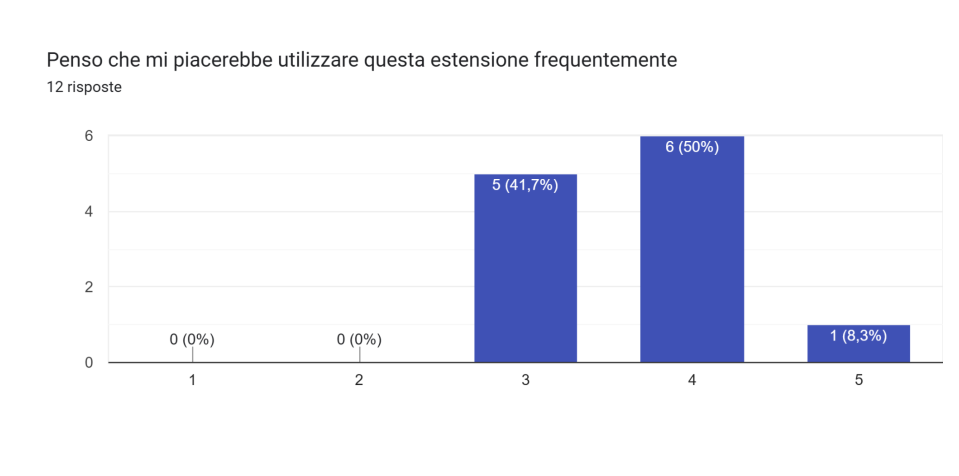
\includegraphics[width=0.95\columnwidth]{sus/domanda_1.png}
    \caption{Risposte alla domanda 1}
    \label{fig:sus_q1}
  \end{figure}
\end{minipage}

\subsubsection*{Domanda 2}

\vspace{5pt}
\begin{minipage}{\textwidth}
  \noindent La figura \ref{fig:sus_q2} mostra le risposte alla seconda domanda del questionario \gls{sus}.
  \begin{figure}[H]
    \centering
    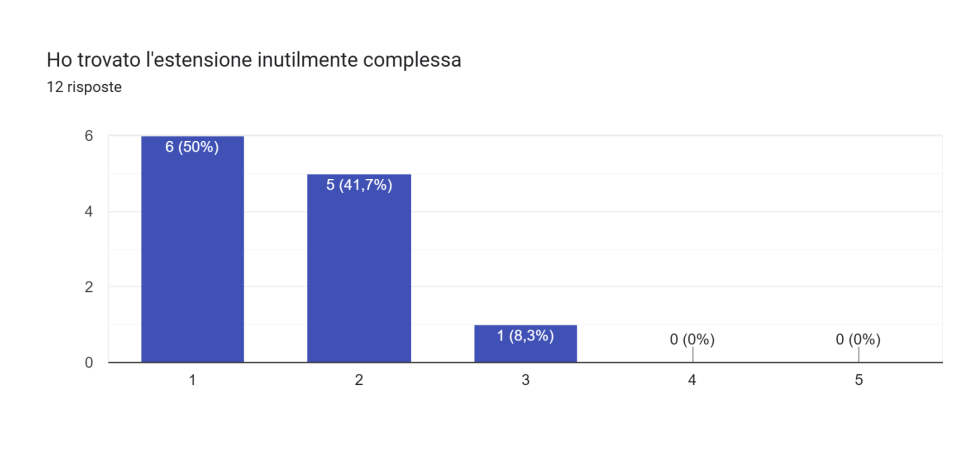
\includegraphics[width=0.95\columnwidth]{sus/domanda_2.png}
    \caption{Risposte alla domanda 2}
    \label{fig:sus_q2}
  \end{figure}
\end{minipage}

\subsubsection*{Domanda 3}

\vspace{5pt}
\begin{minipage}{\textwidth}
  \noindent La figura \ref{fig:sus_q3} mostra le risposte alla terza domanda del questionario \gls{sus}.
  \begin{figure}[H]
    \centering
    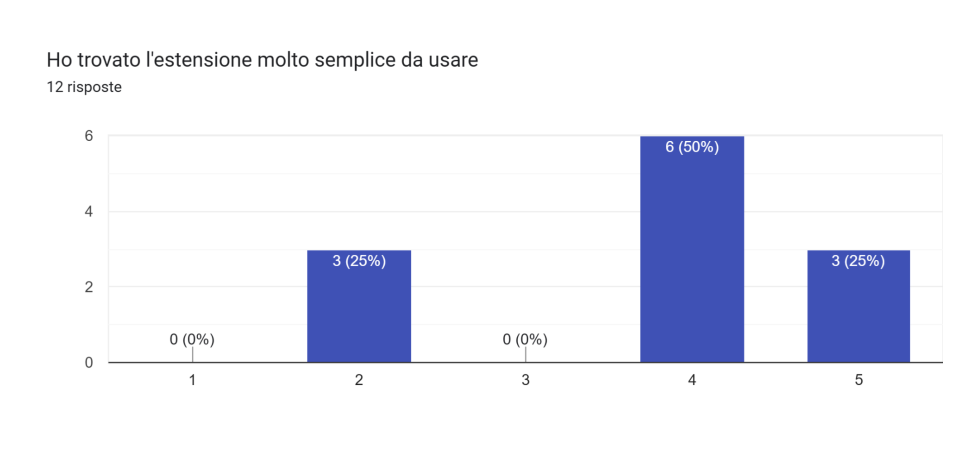
\includegraphics[width=0.95\columnwidth]{sus/domanda_3.png}
    \caption{Risposte alla domanda 3}
    \label{fig:sus_q3}
  \end{figure}
\end{minipage}

\subsubsection*{Domanda 4}

\vspace{5pt}
\begin{minipage}{\textwidth}
  \noindent La figura \ref{fig:sus_q4} mostra le risposte alla quarta domanda del questionario \gls{sus}.
  \begin{figure}[H]
    \centering
    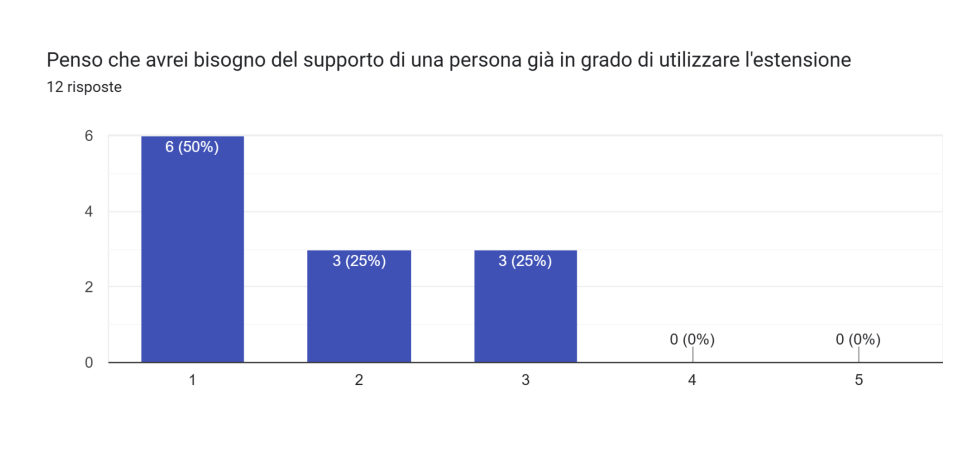
\includegraphics[width=0.95\columnwidth]{sus/domanda_4.png}
    \caption{Risposte alla domanda 4}
    \label{fig:sus_q4}
  \end{figure}
\end{minipage}

\subsubsection*{Domanda 5}

\vspace{5pt}
\begin{minipage}{\textwidth}
  \noindent La figura \ref{fig:sus_q5} mostra le risposte alla quinta domanda del questionario \gls{sus}.
  \begin{figure}[H]
    \centering
    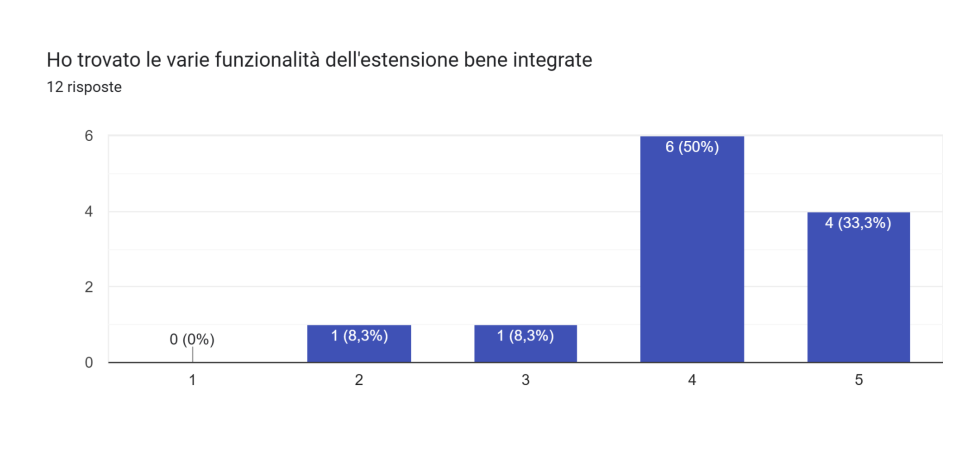
\includegraphics[width=0.95\columnwidth]{sus/domanda_5.png}
    \caption{Risposte alla domanda 5}
    \label{fig:sus_q5}
  \end{figure}
\end{minipage}

\subsubsection*{Domanda 6}

\vspace{5pt}
\begin{minipage}{\textwidth}
  \noindent La figura \ref{fig:sus_q6} mostra le risposte alla sesta domanda del questionario \gls{sus}.
  \begin{figure}[H]
    \centering
    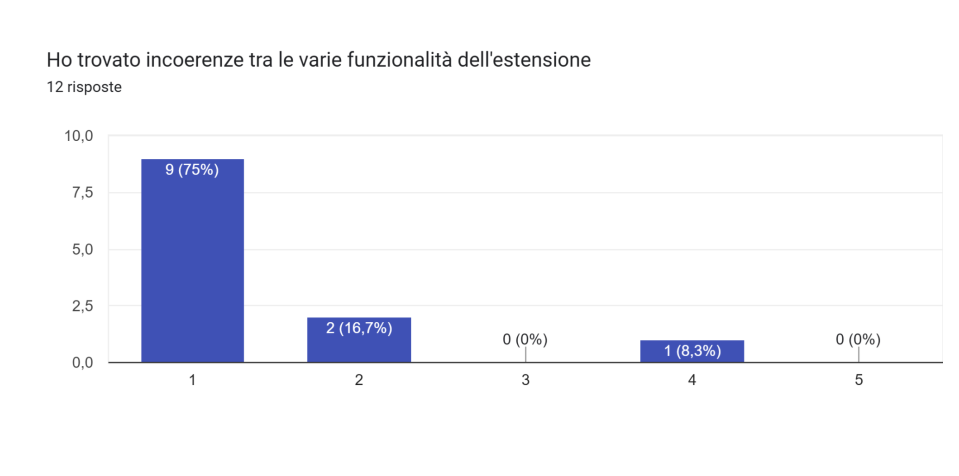
\includegraphics[width=0.95\columnwidth]{sus/domanda_6.png}
    \caption{Risposte alla domanda 6}
    \label{fig:sus_q6}
  \end{figure}
\end{minipage}

\subsubsection*{Domanda 7}

\vspace{5pt}
\begin{minipage}{\textwidth}
  \noindent La figura \ref{fig:sus_q7} mostra le risposte alla settima domanda del questionario \gls{sus}.
  \begin{figure}[H]
    \centering
    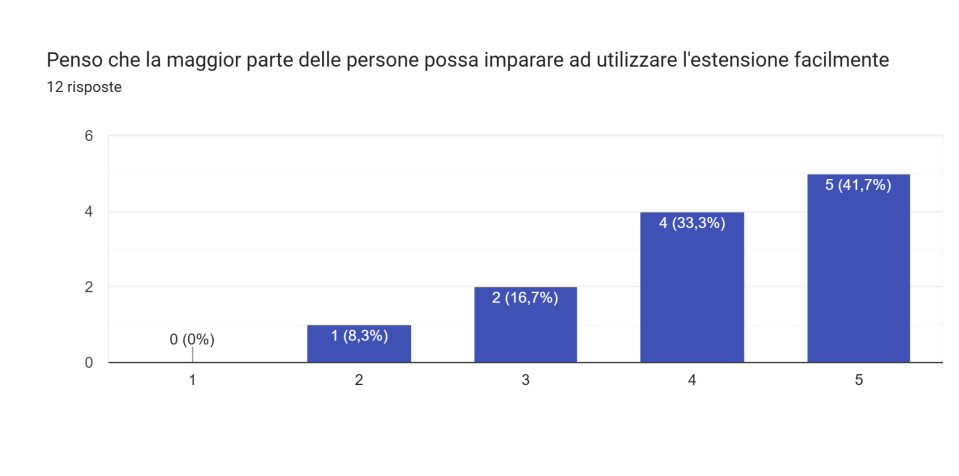
\includegraphics[width=0.95\columnwidth]{sus/domanda_7.png}
    \caption{Risposte alla domanda 7}
    \label{fig:sus_q7}
  \end{figure}
\end{minipage}

\subsubsection*{Domanda 8}

\vspace{5pt}
\begin{minipage}{\textwidth}
  \noindent La figura \ref{fig:sus_q8} mostra le risposte all'ottava domanda del questionario \gls{sus}.
  \begin{figure}[H]
    \centering
    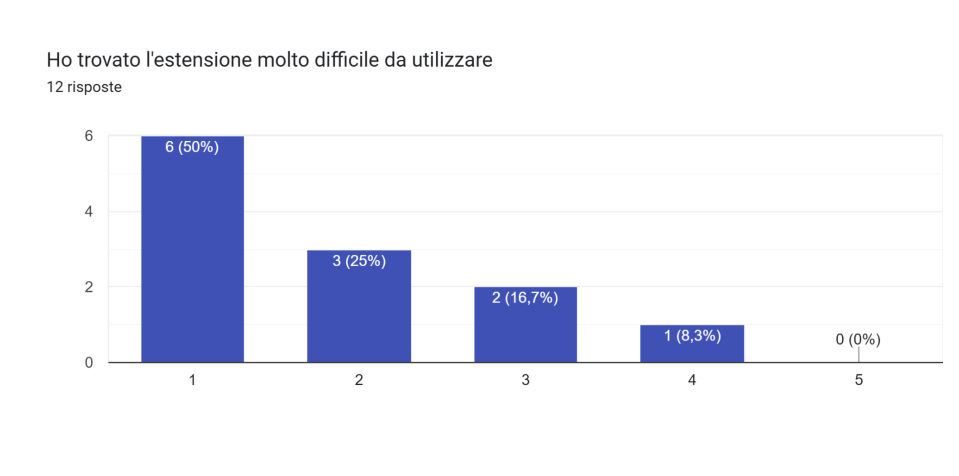
\includegraphics[width=0.95\columnwidth]{sus/domanda_8.png}
    \caption{Risposte alla domanda 8}
    \label{fig:sus_q8}
  \end{figure}
\end{minipage}

\subsubsection*{Domanda 9}

\vspace{5pt}
\begin{minipage}{\textwidth}
  \noindent La figura \ref{fig:sus_q9} mostra le risposte alla nona domanda del questionario \gls{sus}.
  \begin{figure}[H]
    \centering
    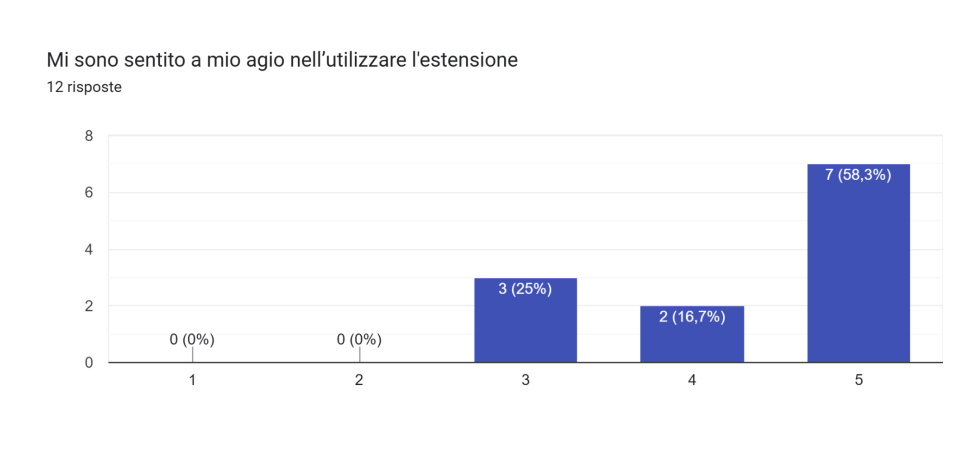
\includegraphics[width=0.95\columnwidth]{sus/domanda_9.png}
    \caption{Risposte alla domanda 9}
    \label{fig:sus_q9}
  \end{figure}
\end{minipage}

\subsubsection*{Domanda 10}

\vspace{5pt}
\begin{minipage}{\textwidth}
  \noindent La figura \ref{fig:sus_q10} mostra le risposte alla decima domanda del questionario \gls{sus}.
  \begin{figure}[H]
    \centering
    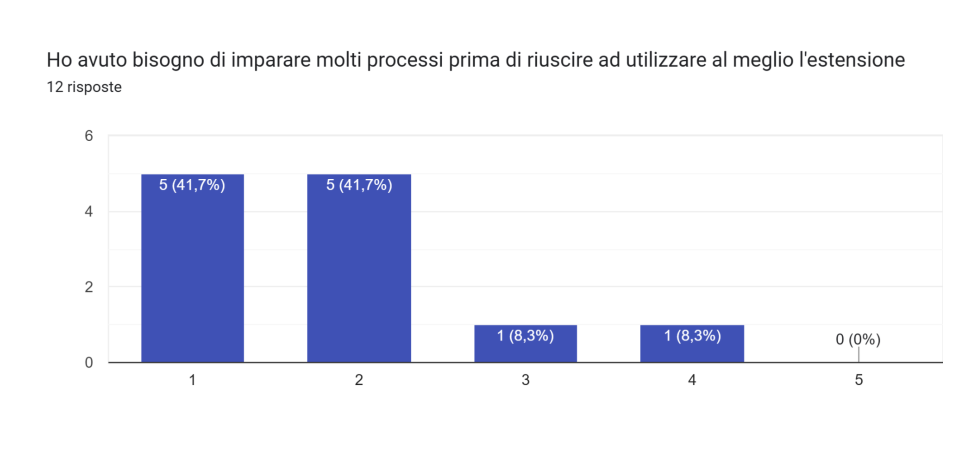
\includegraphics[width=0.95\columnwidth]{sus/domanda_10.png}
    \caption{Risposte alla domanda 10}
    \label{fig:sus_q10}
  \end{figure}
\end{minipage}

\cleardoublepage

\section{Accessibilità}

Dal momento che lo strumento di analisi delle parole chiave è integrato in un’estensione preesistente orientata all’accessibilità, anche questo \textit{tool} è stato progettato in conformità alle linee guida \gls{wcag}. A tal fine, sono stati condotti test di accessibilità con i seguenti obiettivi:
\begin{itemize}
  \item Verificare il rispetto del rapporto minimo di contrasto tra testo e sfondo, pari a 4.5:1 per il testo di dimensioni “normali” e 3:1 per il testo di grandi dimensioni. Questo controllo è stato applicato sia agli elementi interni all’estensione, sia a quelli utilizzati per evidenziare le parole chiave;
  \item Controllare che le immagini non decorative siano dotate di un testo alternativo;
  \item Accertarsi che le icone non decorative siano accompagnate da un’etichetta accessibile;
  \item Verificare l’accessibilità dei tooltip, assicurandosi che vengano attivati e disattivati correttamente quando si interagisce con l’elemento \textit{trigger}, sia tramite navigazione da tastiera sia tramite l’uso del mouse. Inoltre, i tooltip devono rimanere visibili al passaggio del mouse su di essi e devono poter essere chiusi premendo il tasto Esc;
  \item Controllare che tutti gli elementi interattivi (come pulsanti o link) dispongano di un’etichetta testuale descrittiva;
  \item Assicurare la navigazione tramite tastiera, con un ordine di tabulazione logico e una chiara indicazione visiva dell’elemento attualmente attivo.
\end{itemize}

\vspace{15pt}
\noindent Tutti i test eseguiti, sia manuali che automatici (condotti principalmente con \textit{axe DevTools} e \textit{Colour Contrast Analyser}), hanno dato esito positivo.

        %\chapter{Conclusioni}
\label{cap:conclusioni}

\section{Consuntivo finale}

\par Il periodo di stage si è svolto dal 7 aprile al 9 giugno 2025, per un totale di 9 settimane. Rispetto al piano di lavoro standard è stata aggiunta una settimana, interamente dedicata all’analisi delle soluzioni esistenti e alla stesura di una relazione. Nelle prime sei settimane sono state svolte 40 ore di lavoro ciascuna, mentre nelle ultime tre l’impegno è stato di 30 ore settimanali, per un totale complessivo di 330 ore.

\section{Raggiungimento degli obiettivi}

\par Come illustrato nelle tabelle \ref{tab:requisiti-implementazione} e \ref{tab:test-automatici}, tutti i \gls{requisiti} funzionali sono stati soddisfatti, con una copertura del codice e un superamento dei test pari al 100\%. Nella tabella \ref{tab:requisiti-implementazione} sono riportate le classi che hanno contribuito al soddisfacimento di ciascun requisito. Tra i \gls{requisiti} di vincolo, di dominio e di qualità, l’unico obiettivo non raggiunto riguarda l’attivazione automatica dell’estensione su tutte le tab del browser. Questo requisito, previsto nel piano di lavoro e per il quale era stata già progettata l’interfaccia grafica, non è stato implementato per dedicare maggiori risorse al collaudo e all’ottimizzazione delle funzionalità preesistenti.

\section{Conoscenze acquisite}

\par Durante il periodo di stage ho avuto l’opportunità di approfondire i componenti fondamentali per lo sviluppo di un’estensione web: il file \textit{manifest.json}, il \textit{service worker} \textit{(background script)} e il \textit{content script}. In particolare, ho trovato stimolante poter applicare e integrare le conoscenze acquisite durante il percorso accademico - come \gls{api}, \gls{design-pattern}, testing e Chrome DevTools - all’interno di un ambiente di sviluppo moderno, quello delle estensioni.

\vspace{10pt}
\par\noindent Il progetto mi ha permesso di analizzare in profondità il linguaggio \gls{javascript}, che in passato avevo sempre messo in secondo piano rispetto ad \gls{html} e \gls{css}, imparando ad apprezzarne sia le potenzialità che le criticità. Inoltre, ho potuto mettere in pratica le competenze maturate durante il corso di Ingegneria del Software, applicando fin dall’inizio le pratiche di sviluppo in modo attento e consapevole. Questo approccio mi ha aiutato a organizzare il lavoro in modo sostenibile, rispettare le scadenze e comprendere concretamente i vantaggi di una buona progettazione nel lungo periodo, soprattutto nella fase di testing.

\vspace{10pt}
\par\noindent Tra le competenze più significative acquisite durante lo stage, vi è senza dubbio la capacità di integrare nuove funzionalità all’interno di un progetto preesistente, unita alla flessibilità necessaria per adattarsi all’architettura e allo stile definiti da altri sviluppatori. Contribuire a un software non scritto in prima persona ha rappresentato per me una sfida nuova e stimolante, considerando che, nel mio percorso accademico, avevo sempre lavorato a progetti sviluppati “da zero”.

\section{Valutazione personale}

\par Ho trovato questa esperienza estremamente formativa, perché mi ha dato la possibilità di sviluppare un progetto destinato a scenari d’uso concreti, e non esclusivamente orientato alla ricerca teorica, con la consapevolezza del contesto di utilizzo primario. L’estensione, infatti, è pensata come strumento di supporto per la Proponente nella valutazione dei progetti didattici realizzati dagli studenti iscritti al corso di Tecnologie Web. La definizione concreta del contesto di utilizzo mi ha motivato a seguire un modello di sviluppo il più possibile allineato allo “stato dell’arte”, cosa che in passato era avvenuta in modo meno rigoroso o solo parzialmente consapevole. Ritengo che il software realizzato possa costituire una risorsa utile anche per i miei futuri progetti personali.

\vspace{10pt}
\par\noindent Dal punto di vista prettamente teorico, il tirocinio mi ha avvicinato ulteriormente al mondo dell’ottimizzazione \gls{seo}, ambito che avevo già iniziato a esplorare collaborando con una redazione online nella scrittura di blog tramite \gls{wordpress}. Così come rendere i contenuti web accessibili è fondamentale, anche ottimizzarli per migliorarne il posizionamento sui motori di ricerca si è rivelata, grazie a questo progetto, un’attività non solo necessaria ma anche affascinante e intrigante, indipendentemente dal settore digitale di applicazione.

    
        %\appendix
        %\chapter{Appendice A}

\epigraph{Citazione}{Autore della citazione}

    
        \backmatter
        \printglossary[type=\acronymtype, title=Acronimi e abbreviazioni, toctitle=Acronimi e abbreviazioni]
        \printglossary[type=main, title=Glossario, toctitle=Glossario]
    
        \cleardoublepage
\chapter{Bibliografia}

\nocite{*}

% Print book bibliography
\printbibliography[heading=subbibliography,title={Riferimenti bibliografici},type=book]

% Print site bibliography
\printbibliography[heading=subbibliography,title={Siti web consultati},type=online]

    \end{document}
    